\documentclass[a4,12pt]{book}

\usepackage{template}

% Parallelepiped definitions
\usetikzlibrary{quotes,arrows.meta}


\begin{document}

\chapter{Começando a falar sobre frações }

\section{EXPLORANDO O ASSUNTO }

\subsection{Atividade}

Três irmãos vão repartir uma barra de chocolate. Um deles sugere a seguinte divisão: 

\begin{imagem*}[breakable]{}{}   - FIGURA ARTÍSTICA   
  
Na imagem devem estar 3 irmãos, aparentando idades diferentes (um deles pode ser cadeirante, por exemplo), observando uma única barra de chocolate retangular (preferencialemnte,   {\bf imagem tridimensional sem subdivisões}  ) repartida em três partes com tamanhos diferentes. Por exemplo:  
  
    \includegraphics[width=180pt, keepaspectratio]{../../livro/media/cap1/secoes/licao1_1.png}  
  
\end{imagem*}

\begin{enumerate} [\quad a)] %s
  \item     Você concorda com essa divisão? Explique.
  \item     Com essa divisão, os três irmãos receberão a mesma quantidade de chocolate?
  \item     Use a imagem a seguir para mostrar uma divisão da barra de chocolate que permita que os 3 irmãos recebam quantidades iguais de chocolate. 
\begin{imagem*}[breakable]{}{}    - FIGURA ARTÍSTICA - Inserir imagem da mesma barra retangular de chocolate da ilustração anterior sem qualquer partição sugerida. Apenas a imagem da barra de chocolate. Não há necessidade de ilustrar os irmãos.\end{imagem*}
  \item     Considerando a divisão da barra de chocolate em 3 partes iguais, como você nomearia a quantidade de chocolate que cada irmão receberia? 
\end{enumerate} %s

\subsection{Atividade}
Três pizzas inteiras, de mesmo tamanho, foram repartidas entre as crianças de uma turma. Para isso, a turma foi dividida em três grupos com quatro crianças cada. Veja como cada grupo repartiu a sua pizza.

\begin{imagem*}[breakable]{}{}    - FIGURA ARTÍSTICA - A imagem deve conter 3 GRUPOS com 4 CRIANÇAS cada (Diversificar as características físicas das crianças). Cada um dos grupos deve estar observando uma pizza. Colocar duas das crianças do grupo 3 com feições   ``contrariadas''  . As pizzas devem ter mesmos tamanho e formato. As pizzas devem estar repartidas de três maneiras diferentes, como indicado nas imagens a seguir: Grupo 1, Grupo 2 e Grupo 3:   
    \includegraphics[width=300pt, keepaspectratio]{../../livro/media/cap1/secoes/licao1_atv2.png}  
  ilustração: Cambrainha  
\end{imagem*}

\begin{enumerate} [\quad a)] %d
  \item     Cada um dos três grupos repartiu a sua pizza na mesma quantidade de fatias que os outros grupos?
  \item     Dessa maneira, todas as crianças da turma receberam a mesma quantidade de pizza?
  \item     Em algum dos grupos as 4 crianças receberam a mesma quantidade de pizza? Se sim, em qual? Considerando a pizza inteira, como você nomearia cada uma das fatias de pizza desse grupo? 
\end{enumerate} %d

\subsection{Atividade}

Alice quer enfeitar a sala de aula e pretende prender os enfeites utilizando pedaços de barbante. Para isso, quer cortar o barbante em pedaços iguais, para que os enfeites fiquem todos na mesma altura. Ajude Alice a cortar o barbante.

\begin{imagem*}[breakable]{}{}    - FIGURA ARTÍSTICA - Incluir imagem de um pedaço de barbante e de 4 estrelas congruentes, como ilustrado a seguir:  
  Alice é uma menina morena de rabo de cavalo. Ela será um personagem frequente deste livro.  
  {\bf NÃO REPRODUZIR A IMAGEM DO PENSAMENTO DE ALICE}  , mas colocar uma em que apareça uma da estrelas pendurada em um pedaço de barbante.   
  
    \includegraphics[width=180pt, keepaspectratio]{../../livro/media//cap1/secoes/alice_barbante_estrelas.jpg}  
\end{imagem*}

\begin{imagem*}[breakable]{}{}   - FIGURA ARTÍSTICA -  
  \begin{nota*}[breakable]{}{}         
    INCLUIR PÁGINA DE REPRODUÇÃO COM apenas 1 ESTRELA com aproximadamente 15 cm de altura para ser recortada.    
  \end{nota*}  
\end{imagem*}

\section{ORGANIZANDO AS IDEIAS }

Nas atividades anteriores, as quantidades registradas exigiram a partição de uma unidade. Por exemplo, para obter um terço de uma barra de chocolate foi necessário partir a barra de chocolate. Já para obter um quarto de pizza, foi necessário partir a pizza. Outros exemplos aparecem no dia a dia: ``Comprei meio metro de tecido'' ou ``Gastei um terço da minha borracha''.

A barra de chocolate, a pizza e o pedaço de barbante foram partidos em partes iguais. 
Em cada um dos casos, o que foi repartido é chamado {\bf unidade}. Cada uma das partes em que essas unidades foram repartidas igualmente é uma {\bf fração da unidade}. Assim, por exemplo, um quarto de uma pizza é uma fração da pizza e a pizza é unidade. Se a unidade for o pedaço de barbante, um quarto do pedaço de barbante será uma fração do pedaço de barbante.

\begin{imagem*}[breakable]{}{}   - FIGURA ARTÍSTICA -  
  {\bf Imagem de uma pizza e de um pedaço de barbante, cada um dividido em 4 partes.}  
\end{imagem*}

O nome dado à fração da unidade depende da quantidade de partes em que a unidade é dividida. 

Ao dividir uma unidade qualquer em duas partes iguais, ou ao meio, cada uma das partes é chamada de {\it um meio} ou {\it a metade} da unidade. 

Por exemplo, se uma barra de chocolate é repartida igualmente entre dois amigos, a quantidade que caberá a cada um dos amigos é {\it um meio} da barra de chocolate (ou {\it metade} da barra). Nesse exemplo, a unidade é a barra de chocolate.

\begin{imagem*}[breakable]{}{}   - FIGURA ARTÍSTICA - INCLUIR IMAGENS ILUSTRATIVA de metade   
  {\bf Imagem de duas crianças a barra de chocolate em que a metade é identificada}  
\end{imagem*}

Ao dividir uma unidade em três partes iguais, cada uma das partes é chamada de {\it um terço} ou {\it a terça parte} da unidade. 

Por exemplo, se, em uma receita de bolo, é necessário acrescentar {\it um terço} de um litro de leite. Isso significa que, para colocar a quantidade correta de leite na receita, é preciso repartir o litro de leite em três partes iguais e usar apenas uma dessas partes, que é {\it um terço} do litro de leite. Nesse caso, a unidade é um litro de leite.

\begin{imagem*}[breakable]{}{}   - FIGURA ARTÍSTICA - INCLUIR IMAGEM ILUSTRATIVA de terço   
  {\bf Sobre uma mesa, uma garrafa cilindrica cheia de leite e três garrafas iguais ao lado, cada uma com 1/3 da capacidade prennchida.}  
  
  Por exemplo:   
    \includegraphics[width=60pt, keepaspectratio]{../../livro/media//cap1/secoes/litro_de_leite.jpg}  
    \includegraphics[width=60pt, keepaspectratio]{../../livro/media//cap1/secoes/um_terco_de_litro_de_leite.jpg}  
  
\end{imagem*}

Ao dividir uma unidade em quatro partes iguais, cada uma das partes é chamada de {\it um quarto} ou {\it quarta parte} da unidade. 

Por exemplo,
A parte colorida da figura é um quarto da figura. Neste caso, a figura é a unidade.

\begin{imagem*}[breakable]{}{}   - FIGURA ARTÍSTICA - INCLUIR IMAGEM ILUSTRATIVA de quartos  
    \includegraphics[width=120pt, keepaspectratio]{../../livro/media//cap1/secoes/quartos_conexoes.jpg}  
   \end{imagem*}

Da mesma forma, ao dividir uma unidade em cinco partes iguais, cada uma das partes é chamada de {\it um quinto} ou {\it quinta parte} da unidade.

Por exemplo,
\emph{um quinto} de todo ouro pesado nas Casas de Fundição no Brasil era pago em impostos à Coroa Portuguesa. Desta forma, a quantidade de ouro pago em impostos à Coroa Portuguesa era igual a \emph{um quinto} ou a \emph{quinta parte} do ouro pesado nas Casas de Fundição no Brasil.

\begin{imagem*}[breakable]{}{}   - FIGURA ARTÍSTICA - INCLUIR IMAGEM ILUSTRATIVA de quintos   
  {\bf Um homem entregando um saco de ouro a um rei e ficando com outros 4 sacos}  
\end{imagem*}

\section{MÃO NA MASSA }

\subsection{Atividade}

\begin{enumerate} [\quad a)] %s
  \item     Quais dos retângulos a seguir foram repartidos em {\it quartos}? \mbox{} \newline      
 %\vspace{0.2cm}
\begin{center} 
 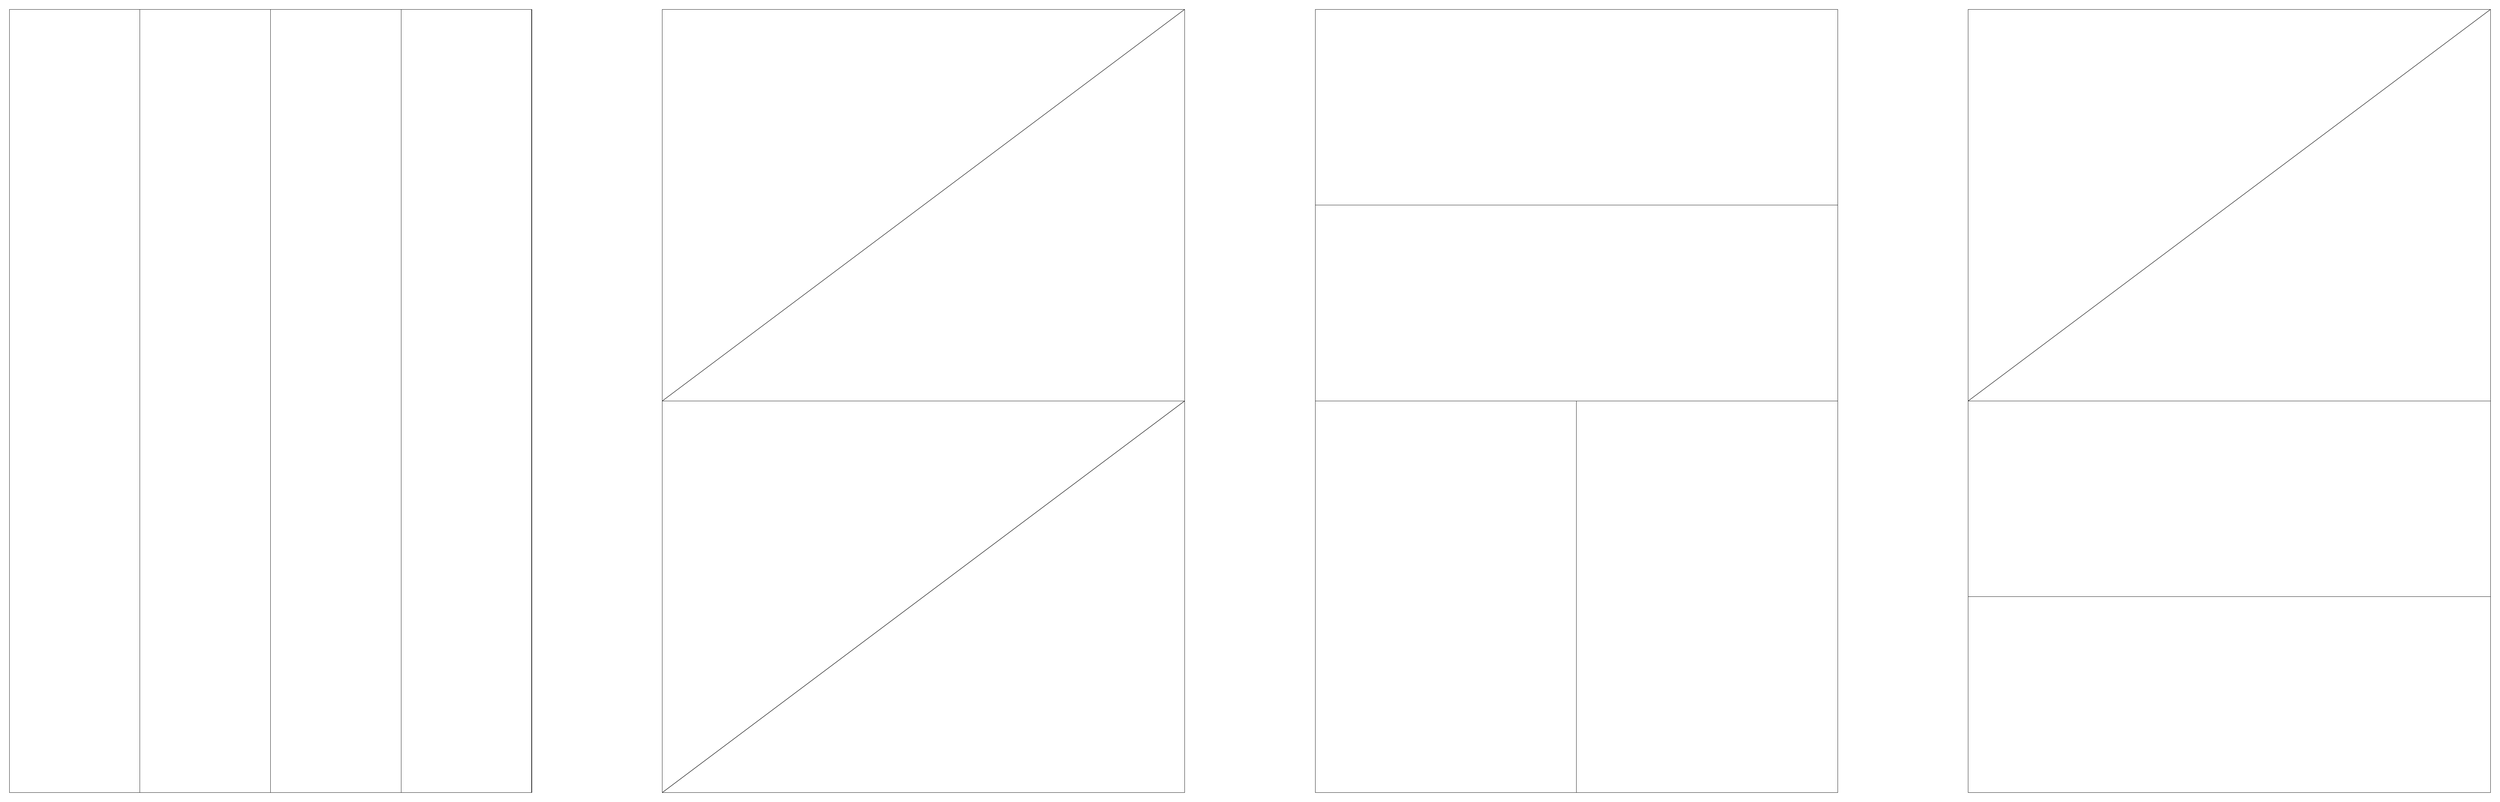
\begin{tikzpicture}[scale=5]
  \draw (0,0) rectangle (1,6);
  \draw (1,0) rectangle (2,6);
  \draw (2,0) rectangle (3,6);
  \draw (3,0) rectangle (4,6);
  \draw (5,0) rectangle (9,3);
  \draw (5,0) rectangle (9,6);
  \draw (5,0) -- (9,3);
  \draw (5,3) -- (9,6);
  \draw (10,0) rectangle (14,3);
  \draw (10,3) rectangle (14,6);
  \draw (12,0) -- (12,3);
  \draw (10,4.5) -- (14,4.5);
  \draw (15,0) rectangle (19,3);
  \draw (15,3) rectangle (19,6);
  \draw (15,1.5) -- (19,1.5);
  \draw (15,3) -- (19,6);
\end{tikzpicture}

\vspace{0.2cm}

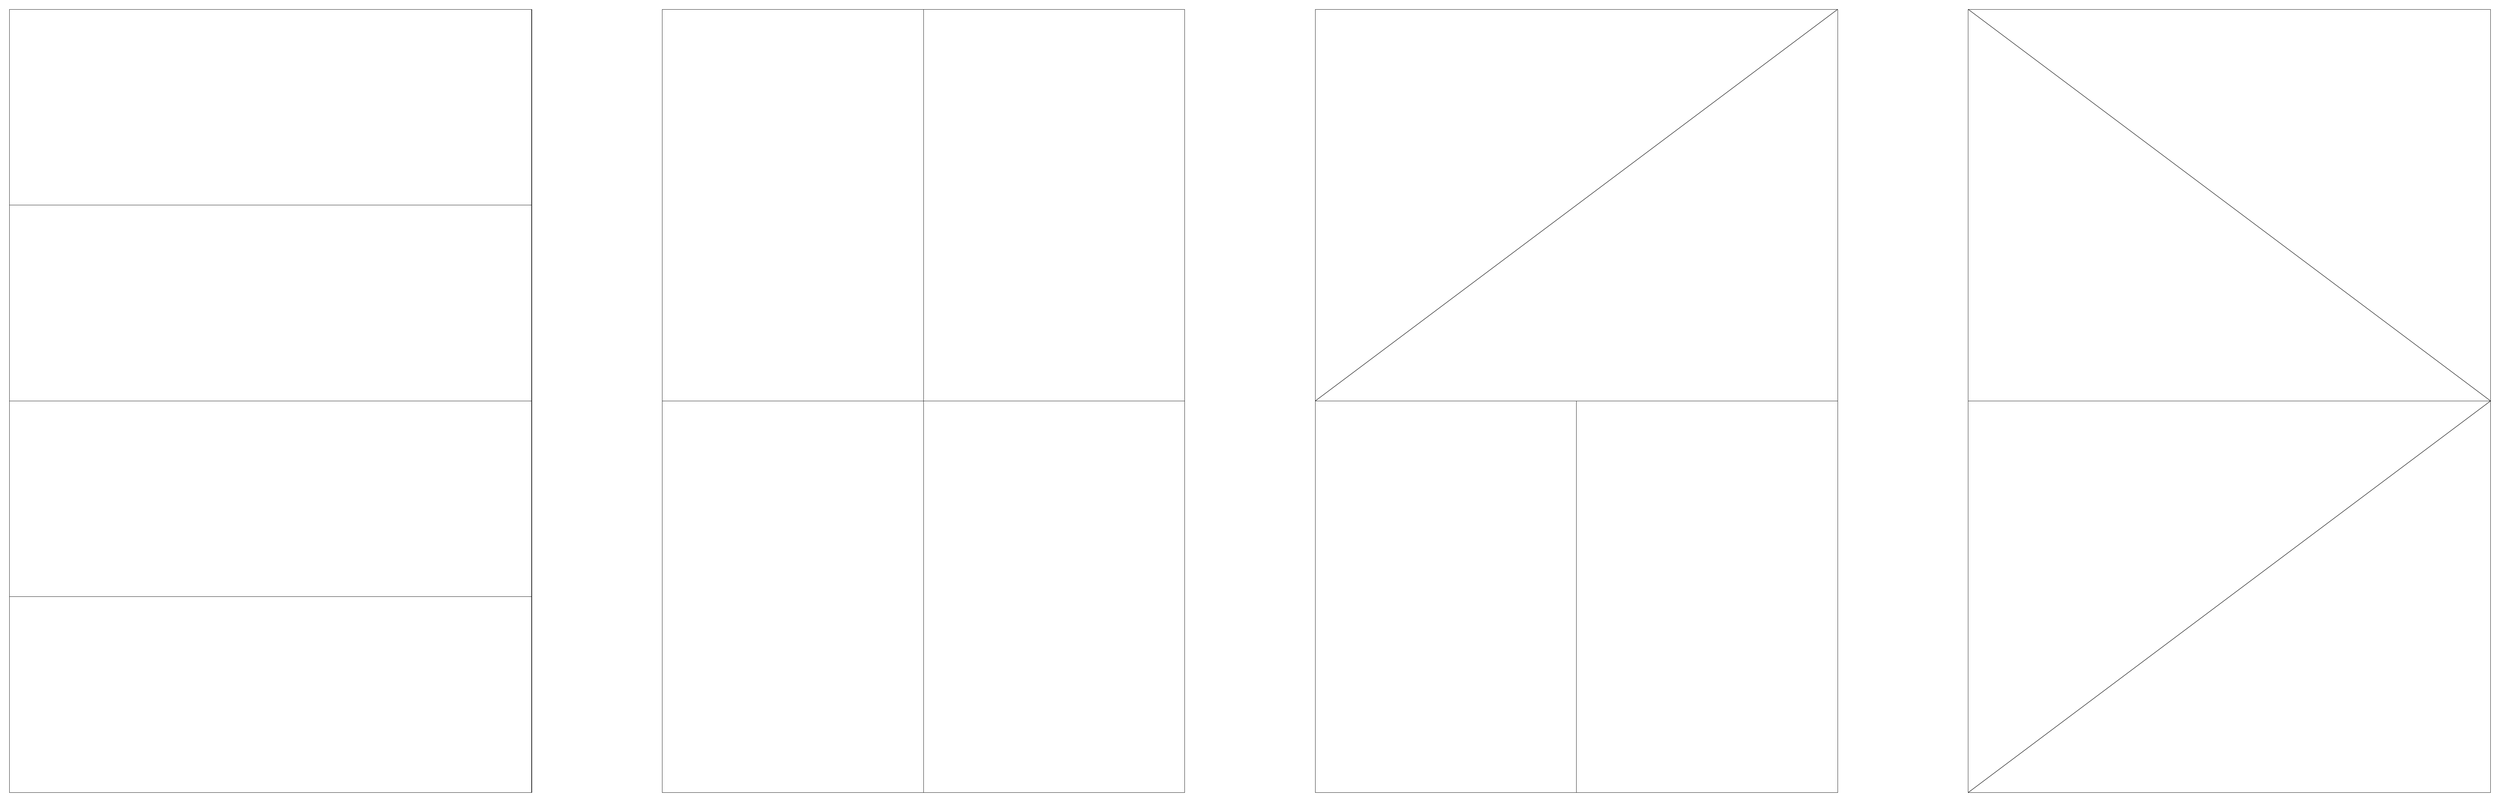
\begin{tikzpicture}[scale=5]
  \draw (0,0) rectangle (4,1.5);
  \draw (0,1.5) rectangle (4,3);
  \draw (0,3) rectangle (4,4.5);
  \draw (0,4.5) rectangle (4,6);
  \draw (5,0) rectangle (9,3);
  \draw (5,0) rectangle (9,6);
  \draw (7,0) -- (7,6);
  \draw (10,0) rectangle (14,3);
  \draw (10,3) rectangle (14,6);
  \draw (12,0) -- (12,3);
  \draw (10,3) -- (14,6);
  \draw (15,0) rectangle (19,3);
  \draw (15,3) rectangle (19,6);
  \draw (15,0) -- (19,3);
  \draw (19,3) -- (15,6);
\end{tikzpicture}
\end{center}

  \item     Desenhe um retângulo e faça uma partição desse retângulo em quatro partes que não sejam todas quartos.
\end{enumerate}

\begin{refletindo*}[breakable]{}{}  
  Quando se diz que uma unidade é repartida em meios, terços, quartos, quintos, etc., a unidade foi repartida em 2, 3, 4, 5, etc., partes iguais.  
  Assim como no dia a dia, neste livro o termo   ``partes iguais''   quer dizer   ``partes com a mesma quantidade''  , mesmo que a unidade não esteja dividida em partes de mesma forma.  
  Na atividade anterior, se os retângulos representassem, por exemplo, bolos, as quatro partes em que foram divididos os retângulos representariam quantidades iguais de bolo.   
  Em alguns retângulos as partes não têm a mesma forma.  
  Veja alguns exemplos curiosos em que as   ``partes iguais''   podem gerar confusão.  
  
  \begin{imagem*}[breakable]{}{}     FIGURA ARTÍSTICA    -   
    {\bf Quadrinho 1:}     Uma menina chega ao balcão de uma loja em que há uma pizza inteira:     
    
    Menina: Bom dia! Metade desta pizza, por favor.     
    
    Vendedor: É pra já, vou cortar para você!    
        
    {\bf Quadrinho 2:}     O vendedor entrega a metade da pizza à menina. Mas ao invés de simplesmente cortada ao meio com um segmento de reta, a pizza foi dividida com um S. A menina olhando com ar espantado.     
            
            \includegraphics[width=80pt, keepaspectratio]{../../livro/media//cap1/secoes/193px-pepperoni_pizza_2_.png}    
    ilustração: Pogrebnoj-Alexandroff
        \includegraphics[width=80pt, keepaspectratio]{../../livro/media//cap1/secoes/pizza_yinyang.png}    
  \end{imagem*}  
  
  \begin{imagem*}[breakable]{}{}     FIGURA ARTÍSTICA   -     Dois amigos terminam de preparar uma torta na cozinha de sua casa e olhando empolgados para a torta diante deles na mesa.    
    
    {\bf Quadrinho 1:}  Menino 1:  Terminamos! Mas agora preciso ir que minha mãe está me esperando. Vou avisá-la que já estou indo.    
    
        \includegraphics[width=80pt, keepaspectratio]{../../livro/media//cap1/secoes/torta_abacaxi1.jpg}    
    
    ilustração: Kimberly Vardeman    
    
    Menino 2: Certo, vou dividir meio a meio para você levar a sua metade com você.    
    
    {\bf Quadrinho 2:}    
    O menino 1 está falando ao telefone afastado e o menino 2 está cortando a torta ao meio. Mas ele está fazendo um corte na horizontal para ficar com todo a cobertura para si.    
  \end{imagem*}  
\end{refletindo*}

\subsection{Atividade}

Em cinco das figuras a seguir a parte em vermelho é um terço da figura. Identifique essas figuras.

\begin{center}
\begin{tabular}{ccc}
a)
\parbox[t][3cm][c]{5cm}{
  \begin{tikzpicture}[scale=0.7]
    \draw[very thick, attention] (90:2 cm)  -- (210:2 cm);
    \draw[very thick, attention] (330:2 cm) -- (90:2 cm);      
    \draw[very thick, common] (210:2 cm)  -- (330:2 cm);
  \end{tikzpicture}
}
& \quad \quad  &

b)
\parbox[t][3cm][c]{5cm}{
\begin{tikzpicture}[scale=6]
  \filldraw[fill=common, draw=black] (0,0) -- (0.5,0.5) -- (3.5,0.5) -- (3.5,2.5) -- (4,3) -- (4,0)--cycle;
  \fill[attention] (0,0) -- (0.5,0.5) -- (0.5,2.5) -- (3.5,2.5) -- (4,3) -- (0,3)--cycle;
  \draw (0,0) rectangle (4,3);
  \draw (0.5,0.5) rectangle (3.5,2.5);
\end{tikzpicture}
}
\\

c)
\parbox[t][3cm][c]{5cm}{
\begin{tikzpicture}[scale=4]
  \draw[very thick, common] (0,3) -- (3,0);
  \draw[very thick, attention] (3,0) -- (6,3);
  \draw[very thick, common] (6,3) -- (9,0);      
\end{tikzpicture}
}
& &

d)
\parbox[t][3cm][c]{5cm}{
\begin{tikzpicture}[scale=0.7]
  \draw[very thick, common] (90:2 cm)  -- (210:2 cm);
  \draw[very thick, attention] (210:2 cm)  -- (330:2 cm);
  \draw[very thick, common] (330:2 cm) -- (90:2 cm);
\end{tikzpicture}
    }\\
  
e)
\parbox[t][3cm][c]{5cm}{
  \begin{tikzpicture}%[scale=60]
  \tikzset{
  annotated cuboid/.pic={
    \tikzset{%
      every edge quotes/.append style={midway, auto},
      /cuboid/.cd,
      #1
    }
    \draw [every edge/.append style={pic actions, densely dashed, opacity=0}, pic actions]
    (0,0,0) coordinate (o) -- ++(-\cubescale*\cubex,0,0) coordinate (a) -- ++(0,-\cubescale*\cubey,0) coordinate (b) edge coordinate [pos=1] (g) ++(0,0,-\cubescale*\cubez)  -- ++(\cubescale*\cubex,0,0) coordinate (c) -- cycle
    (o) -- ++(0,0,-\cubescale*\cubez) coordinate (d) -- ++(0,-\cubescale*\cubey,0) coordinate (e) edge (g) -- (c) -- cycle
    (o) -- (a) -- ++(0,0,-\cubescale*\cubez) coordinate (f) edge (g) -- (d) -- cycle;
 },
  /cuboid/.search also={/tikz},
  /cuboid/.cd,
  width/.store in=\cubex,
  height/.store in=\cubey,
  depth/.store in=\cubez,
  units/.store in=\cubeunits,
  scale/.store in=\cubescale,
  width=100,
  height=100,
  depth=100,
  units=cm,
  scale=.1,
}

    \pic [fill=attention] at (50,0) {annotated cuboid={width=100, height=100, depth=14}};
    \pic [fill=common] at (60,0) {annotated cuboid={width=100, height=100, depth=14}};
    \pic [fill=common] at (70,0) {annotated cuboid={width=100, height=100, depth=14}};
    \end{tikzpicture}
}
&&

f)
\parbox[t][3cm][c]{5cm}{
\begin{tikzpicture}[scale=0.7]
  \fill[attention] (0,0) -- (60:2 cm) -- (120:2 cm) -- (180:2 cm) -- (0,0);
  \filldraw[fill=common, draw=black] (0,0) -- (60:2 cm) -- (0:2 cm) -- (300:2 cm) -- (240:2 cm) -- (180:2 cm) -- (0,0);
  \foreach \x in {0,60,...,300}{
      \draw (\x:2 cm)  -- (\x + 60:2 cm);}
      \draw (0,0)  -- (60:2 cm);
      \draw (0,0)  -- (180:2 cm);
      \draw (0,0)  -- (300:2 cm);
\end{tikzpicture}
}
\\

g)
\parbox[t][3cm][c]{5cm}{
  \begin{tikzpicture}[scale=4]
    \draw[very thick, attention] (0,3) -- (3,0);
    \draw[very thick, attention] (3,0) -- (6,3);
    \draw[very thick, common] (6,3) -- (9,0);      
  \end{tikzpicture}
}
&&
h)
\parbox[t][3cm][c]{5cm}{
\begin{tikzpicture}[scale=3]
    \draw[fill=common] (0,0) rectangle (3,1);
    \draw[fill=attention] (3,0) rectangle (6,1);
    \draw[fill=common] (6,0) rectangle (9,1);
\end{tikzpicture}
}
\\

i)
\parbox[t][3cm][c]{5cm}{
\begin{tikzpicture}[scale=3]
    \draw[fill=common] (0,0) rectangle (2,1);
    \draw[fill=attention] (2,0) rectangle (6,1);
    \draw[fill=common] (6,0) rectangle (9,1);
\end{tikzpicture}
}&&
j)
\parbox[t][3cm][c]{5cm}{
\begin{tikzpicture}[scale=0.7]
 \fill[attention] (162:2 cm) -- (234:2 cm) -- (306: 2 cm) -- (378: 2cm) -- (0,0) -- cycle;
 \filldraw[fill=common, draw=black] (162:2 cm) -- (0,0) -- (378: 2cm) -- (90: 2cm) -- cycle;
  \foreach \x in {90,162,...,378}{
 \draw (\x: 2cm) -- (\x + 72: 2cm);
 \draw (0,0) -- (\x:2cm);}
\end{tikzpicture}
}
\end{tabular}
\end{center}

\subsection{Atividade}

Observe a tabela a seguir. Em cada linha, a primeira coluna, mais à esquerda, exibe figuras que são frações de uma unidade. A coluna do meio indica essas frações. Complete a tabela, fazendo na terceira coluna de cada linha um desenho da unidade correspondente.

\begin{center}
  \begin{tabular}{|m{0.3\linewidth}|m{0.3\linewidth}|m{0.3\linewidth}|}
  \hline
\centering Parte da unidade & \centering Fração da unidade  & \quad\quad\quad Unidade  \\
\hline \hline  
\centering \begin{tikzpicture}[scale=2]
 \draw [fill=common] (0,0) arc (0:90:3) -- (-3,0) -- cycle;
\end{tikzpicture}
&\centering \parbox[c][1.2cm][c]{0.01cm}{  } metade  &  \\
    \hline
\centering\begin{tikzpicture}[scale=2]
\draw [fill=common] (0,0) arc (0:90:3) -- (-3,0) -- cycle;
\end{tikzpicture}        &\parbox[c][1.2cm][c]{0.01cm}{  } \centering   um terço  &  \\
    \hline
\centering \begin{tikzpicture}[scale=2]
\draw [fill=common] (0,0) arc (0:90:3) -- (-3,0) -- cycle;
\end{tikzpicture}        & \centering \parbox[c][1.2cm][c]{0.01cm}{  } um quarto  &  \\ 
    \hline
\centering \begin{tikzpicture}[scale=2]
\draw [fill=common] (0,0) rectangle (3,3);
\end{tikzpicture}
  & \centering \parbox[c][1.2cm][c]{0.01cm}{  } metade  &  \\
    \hline 
\centering \begin{tikzpicture}[scale=2]
\draw [fill=common] (0,0) rectangle (3,3);
\end{tikzpicture}
  & \centering \parbox[c][1.2cm][c]{0.01cm}{  } um terço  &  \\ 
    \hline 
\centering \begin{tikzpicture}[scale=2]
\draw [fill=common] (0,0) rectangle (3,3);
\end{tikzpicture}
 & \centering \parbox[c][1.2cm][c]{0.01cm}{  } um quarto  &  \\ 
    \hline 
\centering \begin{tikzpicture}[scale=2]
\draw  (0,0) -- (3,3);
\end{tikzpicture}
  & \centering \parbox[c][1.2cm][c]{0.01cm}{  } metade  &  \\
    \hline 
\centering \begin{tikzpicture}[scale=2]
\draw  (0,0) -- (3,3);
\end{tikzpicture}
  & \centering \parbox[c][1.2cm][c]{0.01cm}{  } um terço  &  \\
    \hline 
\centering \begin{tikzpicture}[scale=2]
\draw  (0,0) -- (3,3);
\end{tikzpicture}
  & \centering \parbox[c][1.2cm][c]{0.01cm}{  } um quarto  &  \\
    \hline 
\centering \begin{tikzpicture}[scale=2]
\draw [fill=common] (0,0) -- (3,0) -- (-1.5,1.5) -- cycle;
\end{tikzpicture}  & \centering \parbox[c][1.2cm][c]{0.01cm}{  } metade  &  \\
    \hline 
\centering \begin{tikzpicture}[scale=2]
\draw [fill=common] (0,0) -- (3,0) -- (-1.5,1.5) -- cycle;
\end{tikzpicture}  & \centering \parbox[c][1.2cm][c]{0.01cm}{  } um terço  &  \\ 
    \hline 
\centering \begin{tikzpicture}[scale=2]
\draw [fill=common] (0,0) -- (3,0) -- (-1.5,1.5) -- cycle;
\end{tikzpicture}  & \centering \parbox[c][1.2cm][c]{0.01cm}{  } um quarto  &  \\ 
    \hline 
  \end{tabular}
\end{center}


\subsection{Atividade}

\begin{enumerate} [\quad a)] %s
  \item     Pinte metade do quadrado a seguir.
  
  \begin{center}
 \begin{tikzpicture}[x=1mm,y=1mm]  \draw (0,0) rectangle (20,20);  \end{tikzpicture}  
  \end{center}
 
  \item     Pinte um quarto do quadrado a seguir.
  
  \begin{center}
 \begin{tikzpicture}[x=1mm,y=1mm]  \draw (0,0) rectangle (20,20);  \end{tikzpicture}  
  \end{center}

  \item     Pinte um oitavo do quadrado a seguir.
  
  \begin{center}
 \begin{tikzpicture}[x=1mm,y=1mm]  \draw (0,0) rectangle (20,20);  \end{tikzpicture}  
  \end{center}
  \item     Observando os quadrados pintados nos itens, qual é a maior das frações do quadrado: metade, quarto ou oitavo?
\end{enumerate} %s


\subsection{Atividade}

\begin{enumerate} [a)] %d
  \item     Pinte metade da figura.
\begin{center}  
  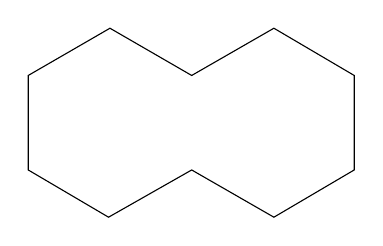
\begin{tikzpicture}[x=1cm,y=1cm, scale=0.6]
  \draw (3.,5.) -- (3.,3.) -- (4.7,2.) -- (6.46,3.) -- (8.2,2.) -- (9.9,3.) -- (9.9,5.) -- (8.2,6.)       -- (6.46,5.) -- (4.73,6.) -- cycle;
  \end{tikzpicture}
\end{center}  

  \item     Pinte metade da figura de forma diferente da do item anterior. 
\begin{center}  
  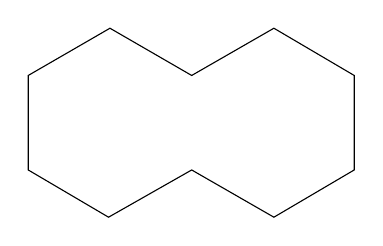
\begin{tikzpicture}[x=1cm,y=1cm, scale=0.6]
  \draw (3.,5.) -- (3.,3.) -- (4.7,2.) -- (6.46,3.) -- (8.2,2.) -- (9.9,3.) -- (9.9,5.) -- (8.2,6.)       -- (6.46,5.) -- (4.73,6.) -- cycle;
  \end{tikzpicture}
\end{center}  

  \item     Pinte a metade da figura de forma diferente das dos dois itens anteriores.     
\begin{center}  
  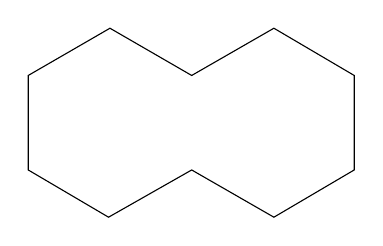
\begin{tikzpicture}[x=1cm,y=1cm, scale=0.6]
  \draw (3.,5.) -- (3.,3.) -- (4.7,2.) -- (6.46,3.) -- (8.2,2.) -- (9.9,3.) -- (9.9,5.) -- (8.2,6.)       -- (6.46,5.) -- (4.73,6.) -- cycle;
  \end{tikzpicture}
\end{center}  
  
  
\end{enumerate} %d


\subsection{Atividade}

Identifique as figuras em que a parte pintada é a metade da figura.

\begin{center}
  \begin{tabular}{ccccc} 
%retângulos

\begin{tikzpicture}[scale=5]
 \draw[fill=common] (0,0) rectangle (3,2);
 \draw (3,0) rectangle (6,2); 
 \node at (3,-1) {Figura 1};
\end{tikzpicture}
&
\quad \quad \quad
&
\begin{tikzpicture}[scale=5]
 \draw (0,0) rectangle (3,2);
 \draw (1,0) -- (1,2);
 \draw (1.5,0) -- (1.5,2);
 \draw (2.2,0) -- (2.2,2);
 \draw[fill=common] (3,0) rectangle (6,2) (3,-1) node{Figura 2};
\end{tikzpicture}
&
\quad \quad \quad
&

\begin{tikzpicture}[scale=5]
 \draw (0,0) rectangle (3,2);
 \draw (3,0) rectangle (6,2) (3,-1) node{Figura 3};
 \filldraw[fill=common, draw=black] (0,2) rectangle (6,1.2);
 \end{tikzpicture}
\\
 % círculos

\begin{tikzpicture}[scale=5]
  \filldraw[fill=common, draw=black] (0,-2) arc (-90:90: 2);
  \draw (0, 2) -- (0, -2);
  \draw (0,2) arc (90:270:2) (0,-3) node{Figura 4};
\end{tikzpicture}
&& 

\begin{tikzpicture}[scale=5]
 \filldraw[fill=common, draw=black] (45:2) arc (45:225:2);
 \draw (225:2) arc (225:405:2) (0,-3) node{Figura 5};
 \draw (0,0) -- (0,-2);
 \draw (0,0) -- (-30:2);
 \draw (225:2) -- (45:2);
 \end{tikzpicture}

 &&
 \begin{tikzpicture}[scale=5]
 \draw (0,0) circle (2);
 \filldraw[fill=common, draw=black] (0,0) -- (2,0) arc (0:90:2) -- cycle; 
 \filldraw[fill=common, draw=black] (0,0) -- (-2,0) arc (180:270: 2) -- cycle;
 \node at (0,-3) {Figura 6};
\end{tikzpicture} 
\\
% hexágonos

\begin{tikzpicture}[scale=5]
 \foreach \x in {0,60,...,300}{
 \draw (\x:2) -- (\x +60: 2);}
 \filldraw[fill=common, draw=black] (2,0) -- (60:2) -- (300:2);
 \node at (0,-3) {Figura 7};
\end{tikzpicture}
& &

\begin{tikzpicture}[scale=5]
  \fill[common] (60:2) -- (120:2) -- (180:2) -- (240:2) --cycle;
  \draw \foreach \x in {0,60,...,300} {(\x:2) -- (\x +60: 2) --(\x +120:2)};
  \draw (60:2) -- (0,0) -- (240:2) (0,-3);
  \draw (2,0) -- (0,0) -- (300:2) (0,-3) node{Figura 8};
\end{tikzpicture}
&&

\begin{tikzpicture}[scale=5]
  \filldraw[fill=common] (0:2) -- (60:2) -- (0:0) --cycle;
  \filldraw[fill=common] (120:2) -- (180:2) -- (0:0) --cycle;
  \filldraw[fill=common] (240:2) -- (300:2) -- (0:0) --cycle;
  \draw \foreach \x in {0,60,...,300}{(\x:2) -- (\x +60: 2)};
  \node at (0,-3) {Figura 9};
\end{tikzpicture}
\\
%círculo

\begin{tikzpicture}[scale=5]
 \draw[fill=common] (0:2) arc (0:270:2) -- (0,0) -- cycle;
 \draw (270:2) arc (270:360:2);
 \draw (0,0) -- (0,-2);
 \draw (0,0) -- (2,0)  (0,-3) node{Figura 10};
 \end{tikzpicture}
&&
%hexágonos

\begin{tikzpicture}[scale=5]
  \fill[common] (120:2) -- (180:2) -- (240:2) -- cycle;
  \fill[common] (240:2) -- (300:2) -- (60:2) -- cycle;
  \draw (120:2) -- (180:2) (180:2) -- (240:2) (240:2) -- (120:2);
  \draw (240:2) -- (300:2) (300:2) -- (60:2) (60:2) -- (240:2);
  \draw \foreach \x in {0,60,...,300}{(\x:2) -- (\x +60: 2) -- (\x +120:2)};
  \node at (0,-3) {Figura 11};
\end{tikzpicture}
&&
%retângulo
\begin{tikzpicture}[scale=5]
 \filldraw[fill=common, draw=black] (1,-1) rectangle (4,1);
 \draw (0,-1) rectangle (6,1);
 \node at (3,-2) {Figura 12};
 \end{tikzpicture}

\end{tabular}
\end{center}


\subsection{Atividade}


Usando os Círculos de Frações, responda:

\begin{center}
 
 \begin{tabular}{ccccc}

 \begin{tikzpicture}
\fill[attention] (0,0) circle (10);
 \end{tikzpicture}
& \parbox[t][.6cm][c]{1cm}{ }\quad\quad\quad\quad&
 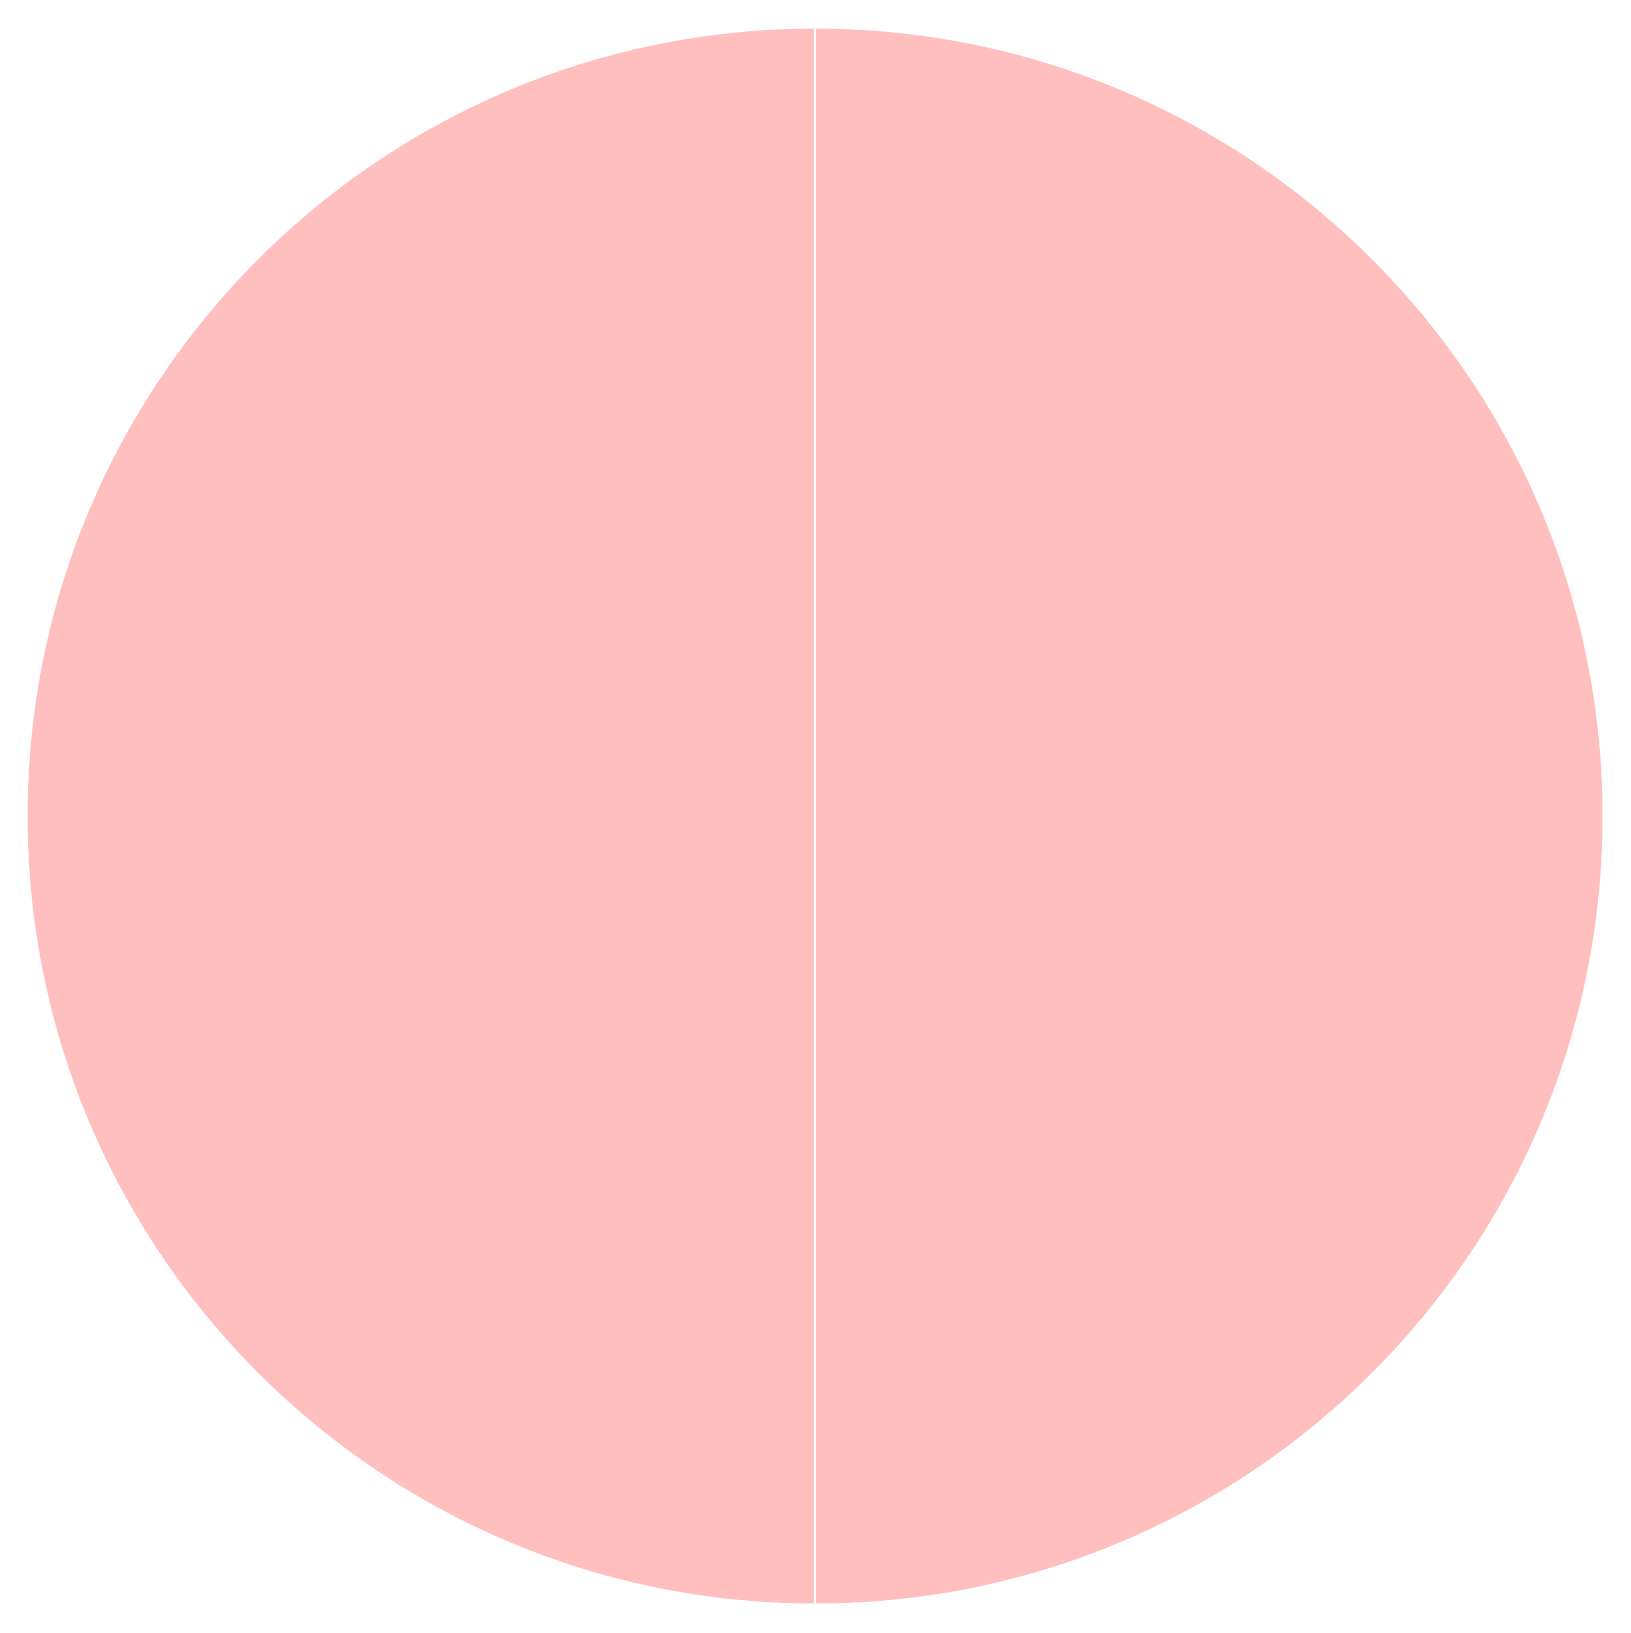
\begin{tikzpicture}
\fill[pink] (0,0) circle (10);
\draw[line width =.25mm, white] (-90:10) -- (90:10);	
\end{tikzpicture}
& \quad\quad\quad\quad&
 
\begin{tikzpicture}
\fill[orange] (0,0) circle (10);
\foreach \x in {30,150,270} \draw[line width =.25mm, white] (0,0)--(\x:10);
\end{tikzpicture}
\\
 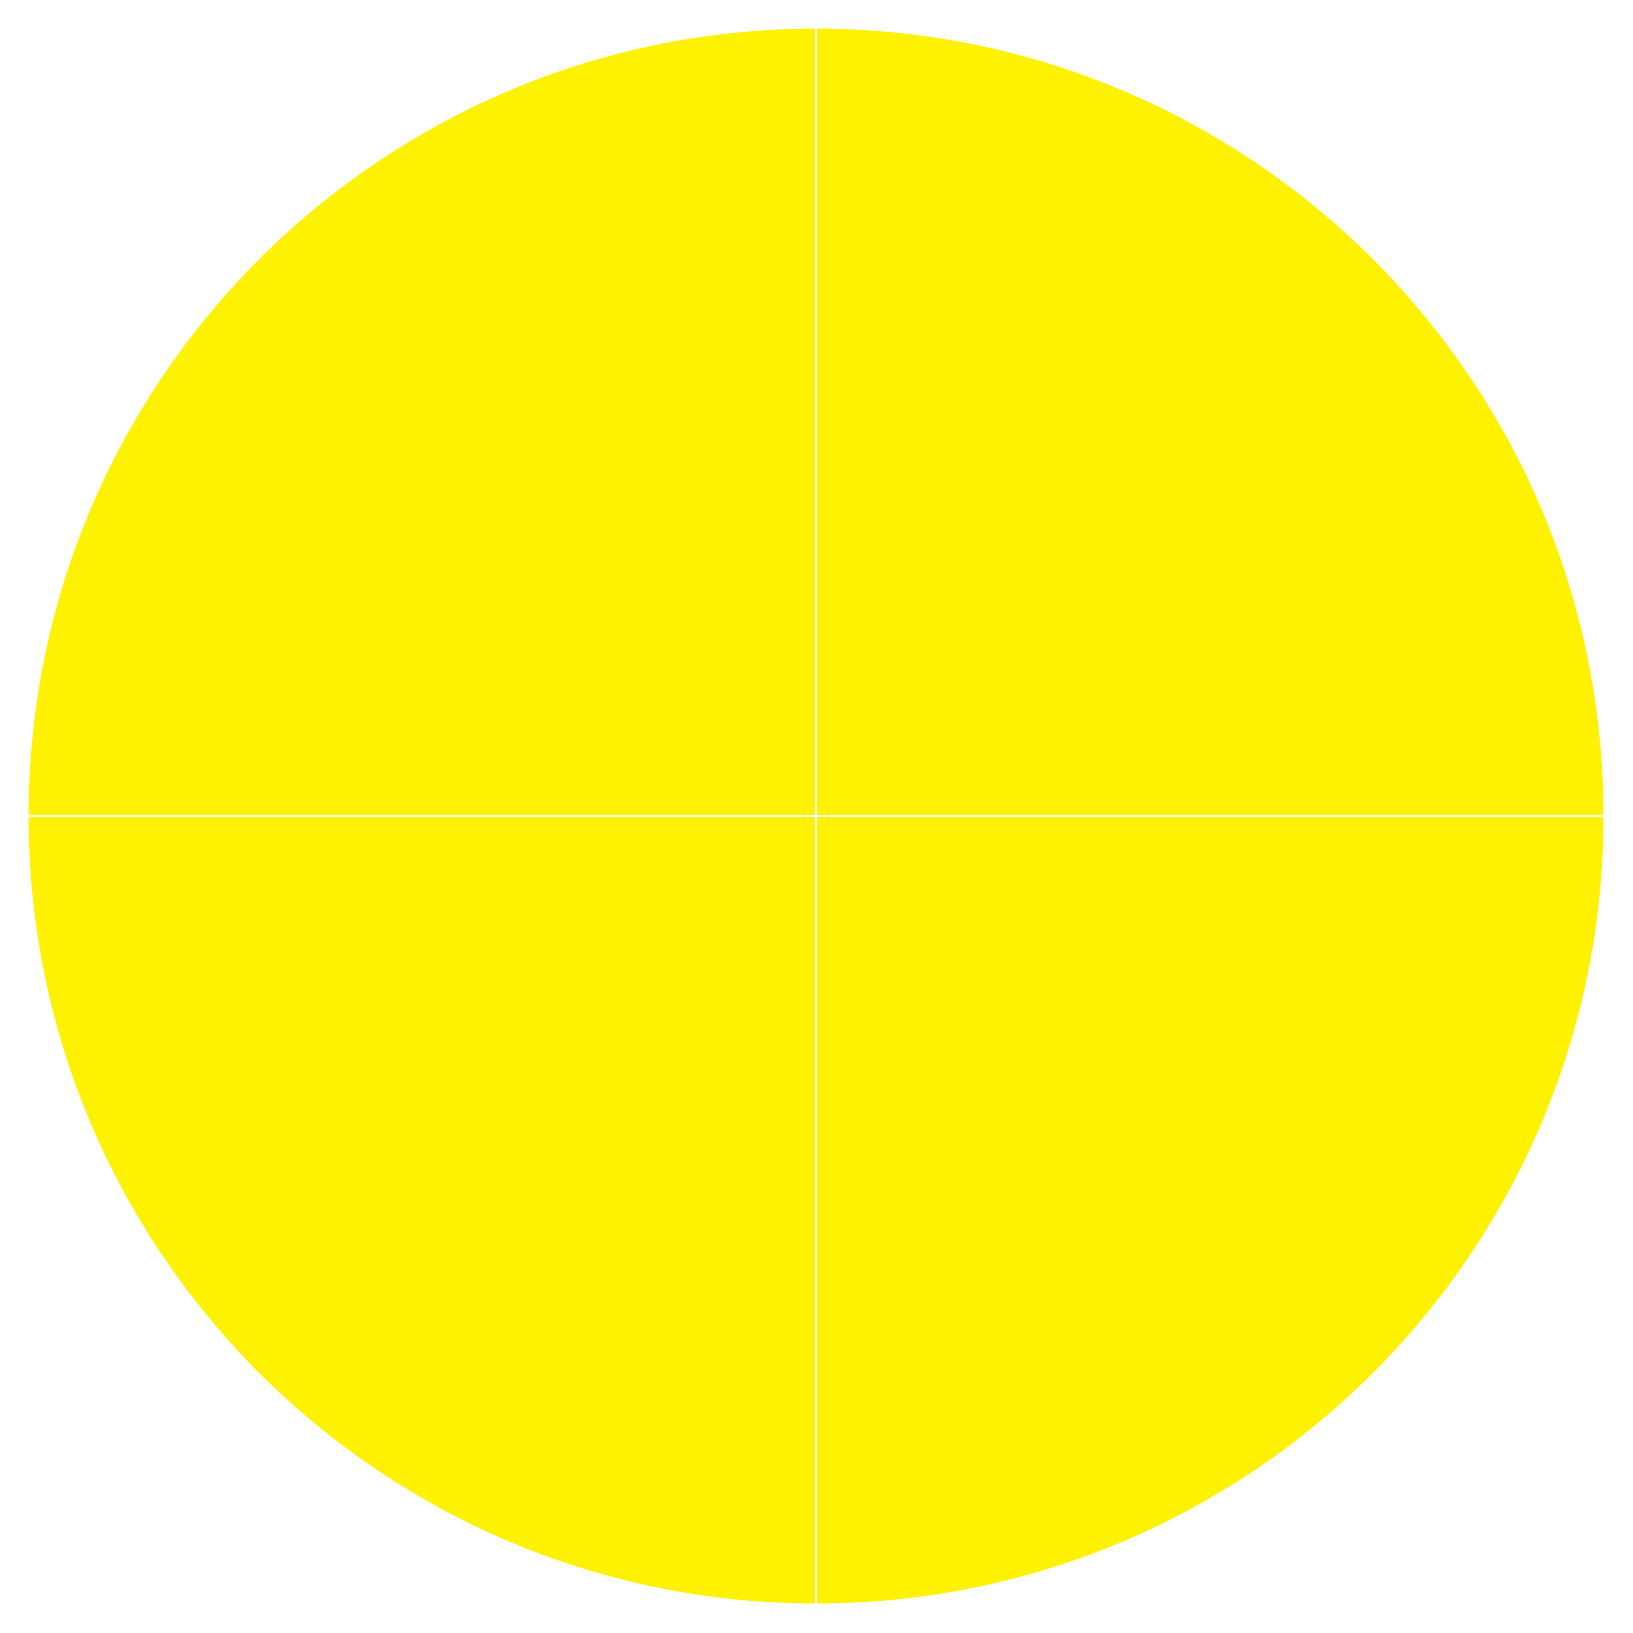
\begin{tikzpicture}
\fill[yellow] (0,0) circle (10);
\foreach \x in {0,90} \draw[line width =.25mm, white] (\x:-10)--(\x:10);
\end{tikzpicture}
&\parbox[t][.6cm][c]{1cm}{ }&
 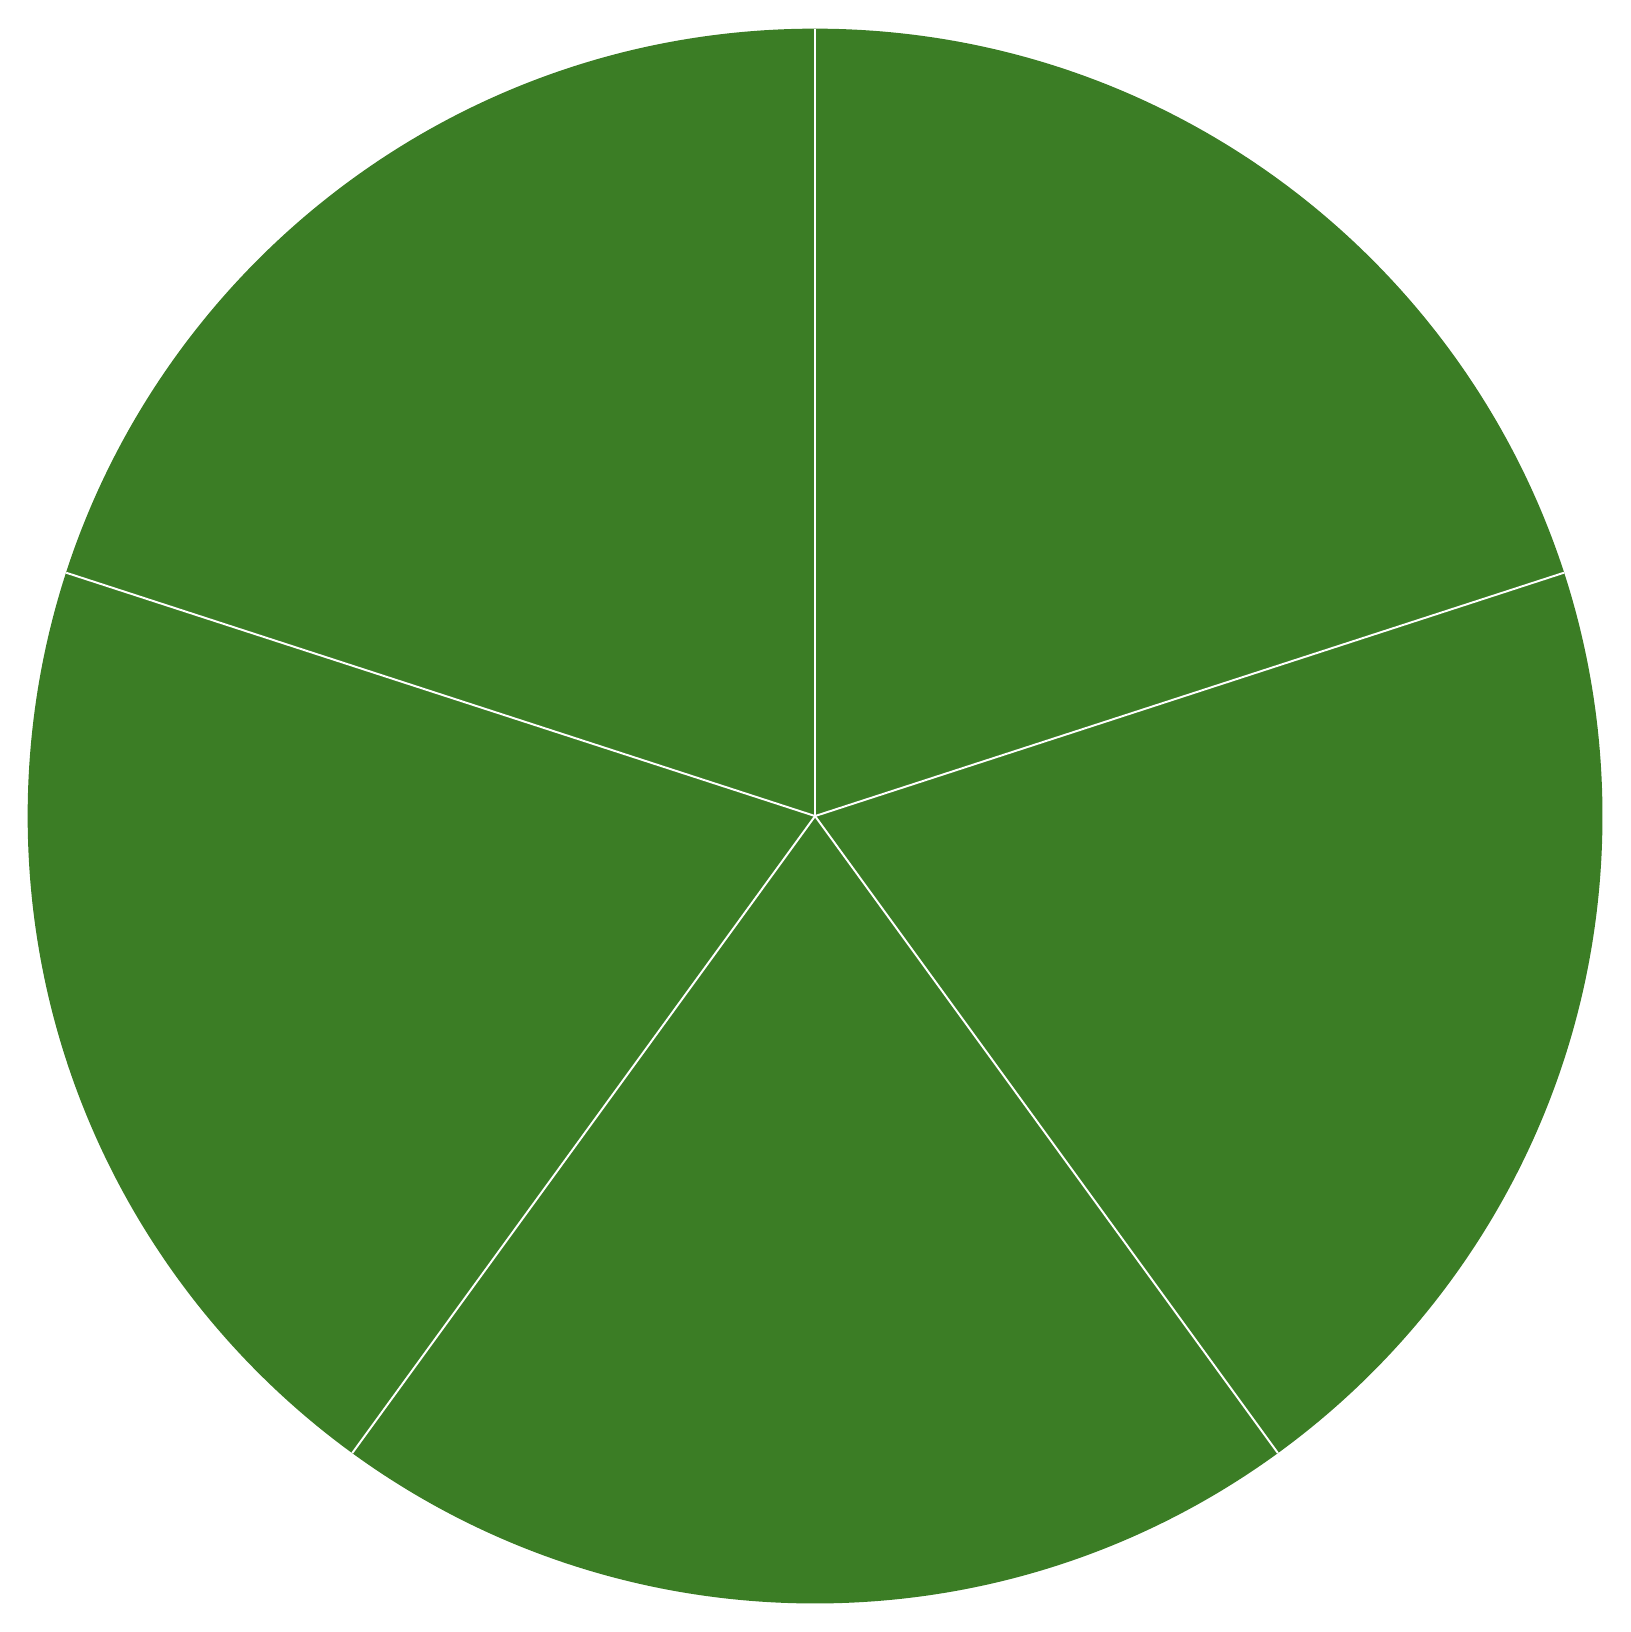
\begin{tikzpicture}
\fill[OliveGreen] (0,0) circle (10);
\foreach \x in {18,90,...,360} \draw[line width =.25mm, white] (0,0)--(\x:10);
\end{tikzpicture}
&&
\begin{tikzpicture}
\fill[common] (0,0) circle (10);
\foreach \x in {0,60,...,360} \draw[line width =.25mm, white] (0,0)--(\x:10);
\end{tikzpicture}
\\
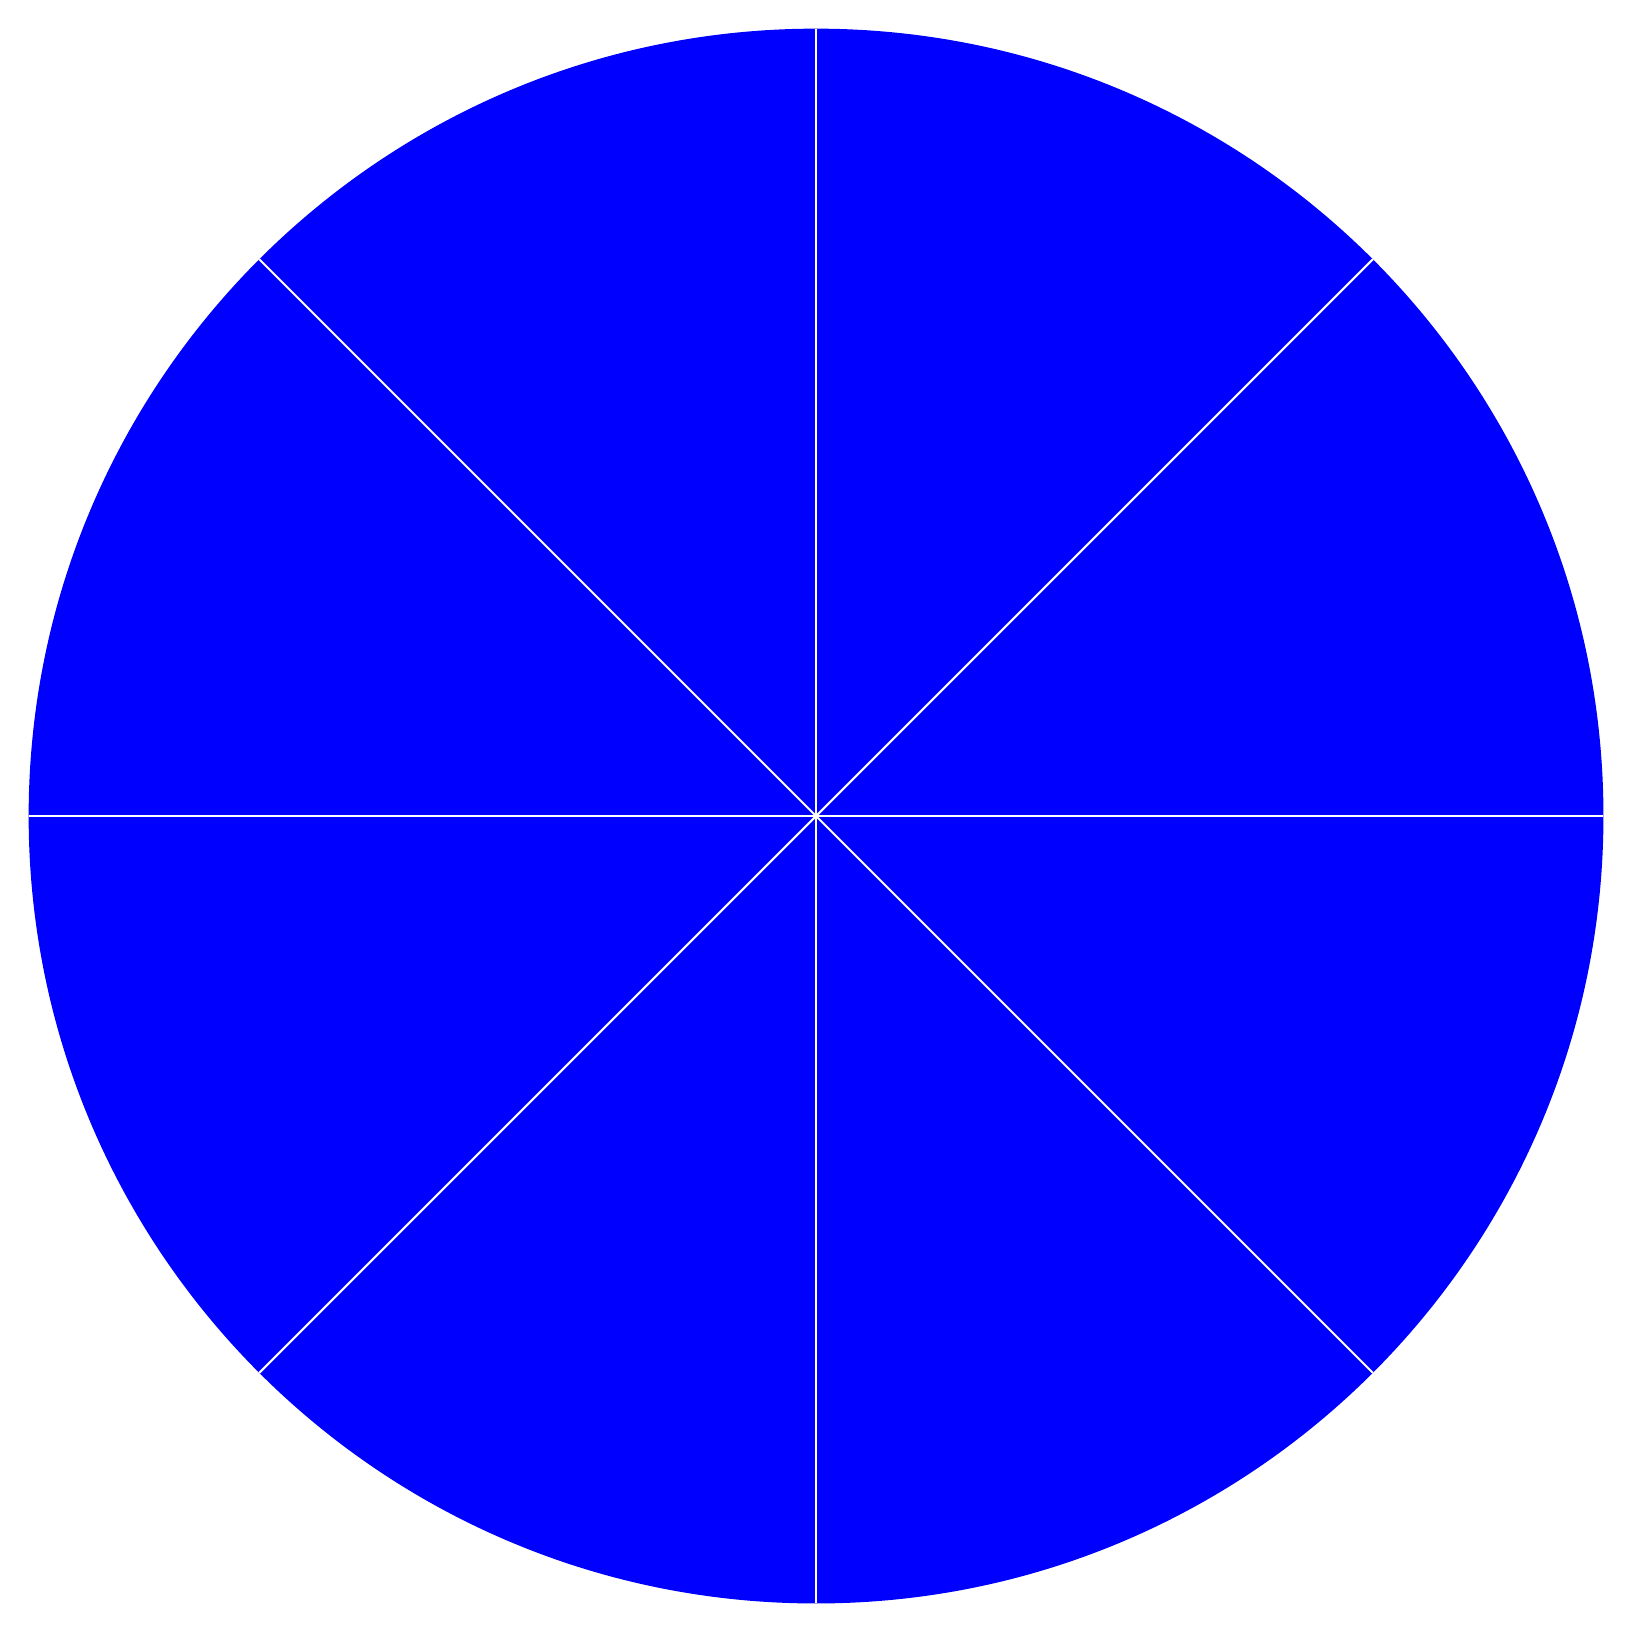
\begin{tikzpicture}
\fill[Blue] (0,0) circle (10);
\foreach \x in {0,45,...,360} \draw[line width =.25mm, white] (0,0)--(\x:10);
\end{tikzpicture}
&\parbox[t][.6cm][c]{1cm}{ }&
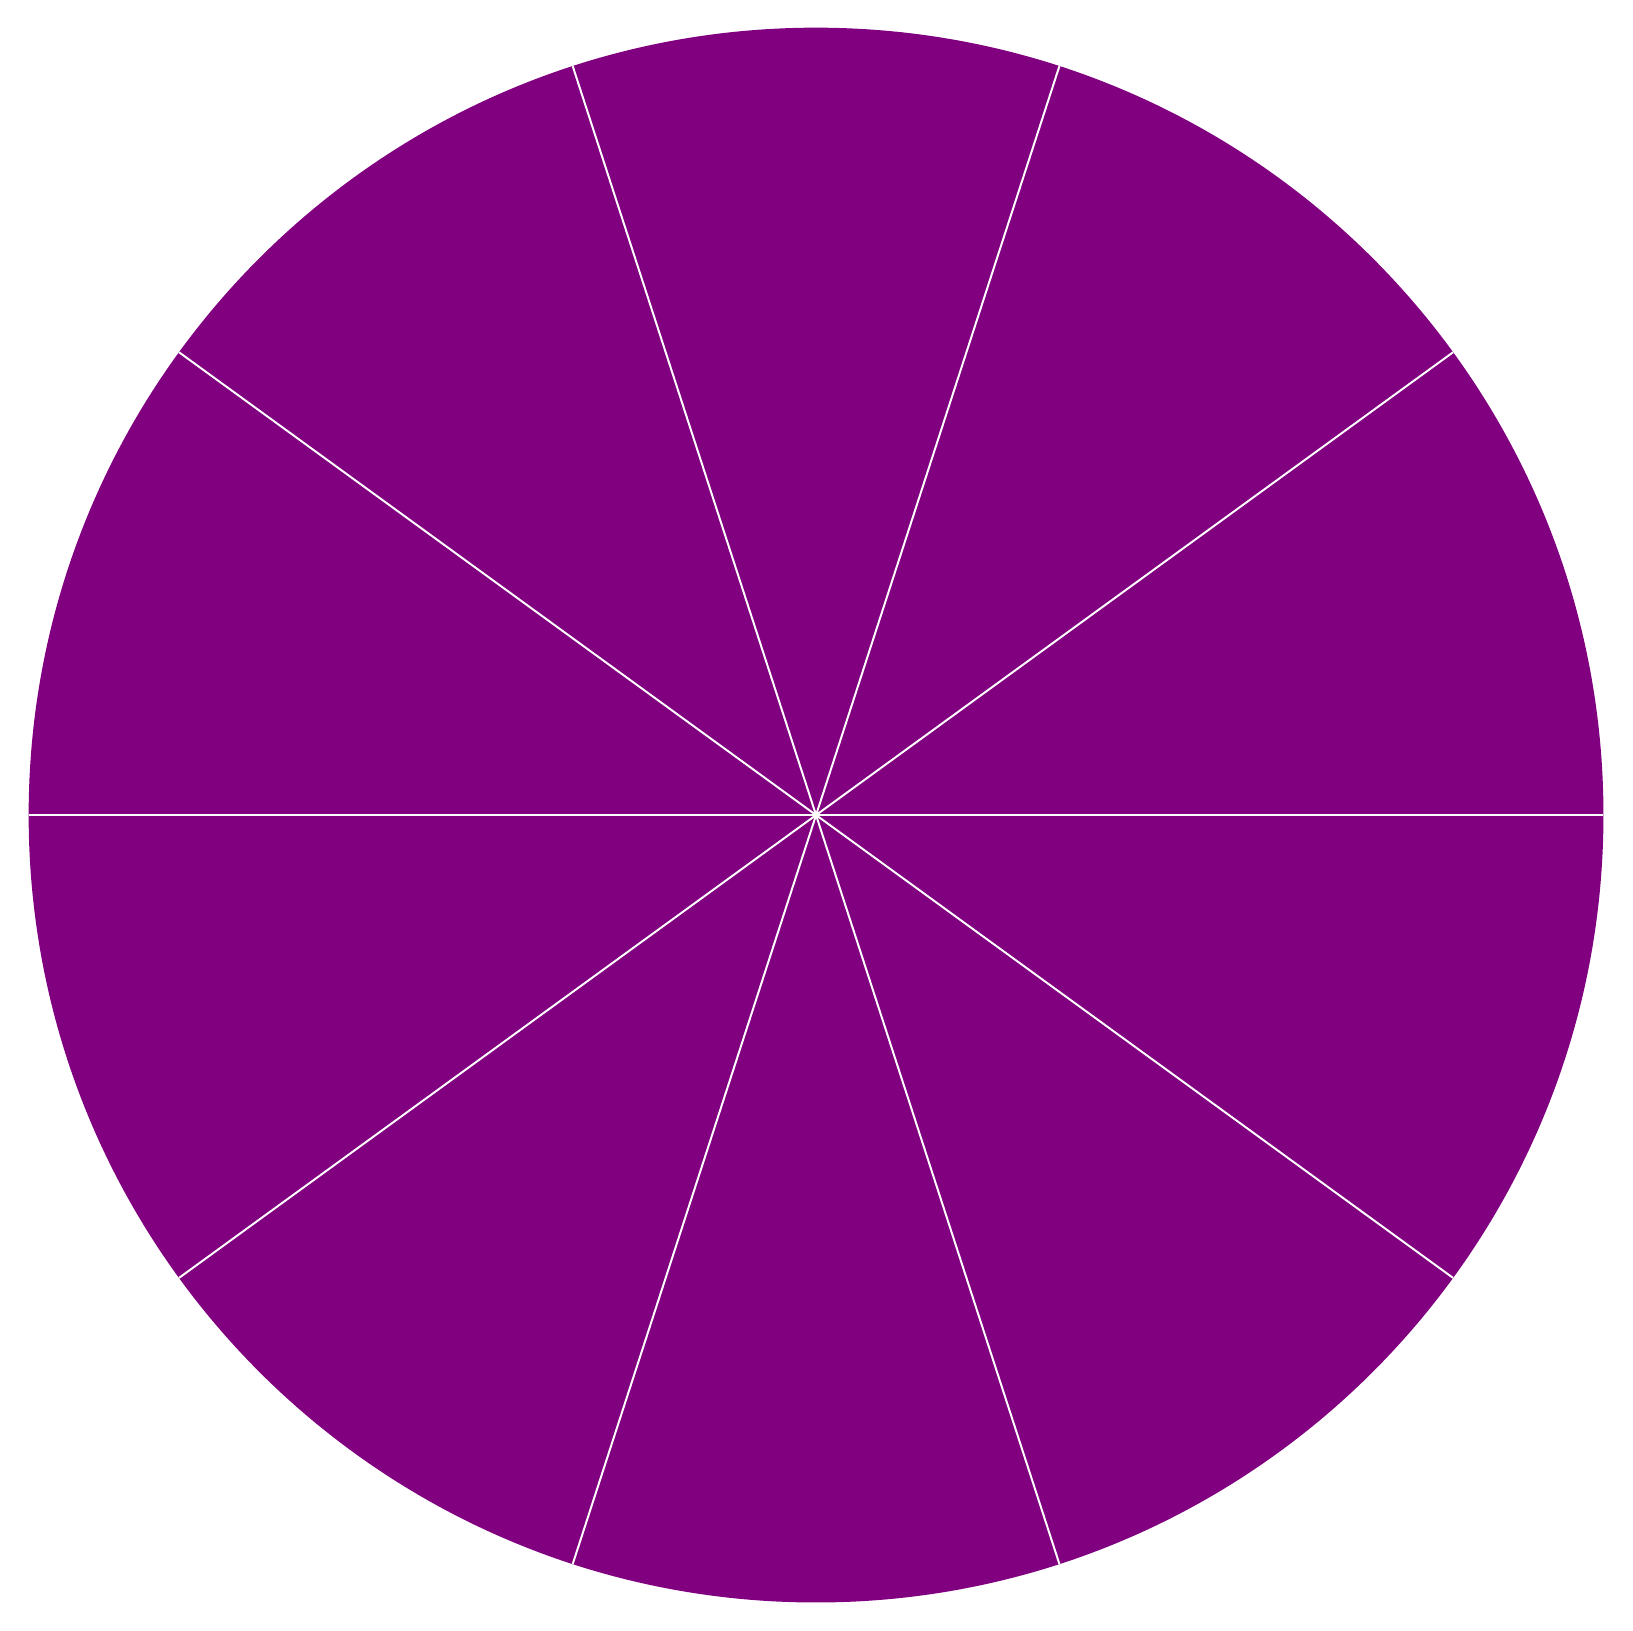
\begin{tikzpicture}
\fill[Purple] (0,0) circle (10);
\foreach \x in {0,36,...,360} \draw[line width =.25mm, white] (0,0)--(\x:10);
\end{tikzpicture}
&&
\begin{tikzpicture}
\fill[black] (0,0) circle (10);
\foreach \x in {0,30,...,360} \draw[line width =.25mm, white] (0,0)--(\x:10);
\end{tikzpicture}

\end{tabular}

\end{center}


\begin{enumerate}[a)]
   \item  Qual a cor da peça que é igual a um terço do círculo preto?
  \item  Qual a cor do peça que é igual a um quarto do círculo preto?
  \item  Qual a cor do peça que é igual a um sétimo do círculo preto?
  \item  Qual a cor do peça que é igual a um nono do círculo preto?
  \item  Que fração do círculo preto é igual a uma peça da cor roxa?
  \item  Que fração do círculo preto é igual a uma peça da cor cinza?
  \item  Que fração do círculo preto é igual a uma peça da cor branco?
  \item  Que fração do círculo preto é igual a uma peça da cor rosa?
  \item  Qual fração do círculo preto é maior, um terço ou um sétimo. Explique a sua resposta.
  \item  Qual fração do círculo preto é menor, um nono ou um quarto. Explique a sua resposta.
  \item  Qual fração do círculo preto é menor, um quinto ou um sétimo. Explique a sua resposta.
  \item  Qual fração do círculo preto é maior, um oitavo ou um quarto. Explique a sua resposta.
  \item  Qual fração do círculo preto é maior, um sexto ou um sétimo. Explique a sua resposta.
\end{enumerate}

\subsection{Atividade}







Nas figuras a seguir, um mesmo círculo aparece diferentemente dividido em partes iguais. 
\begin{enumerate} [\quad a)] %s
  \item     Complete as sentenças a seguir identificando os círculos que as tornam verdadeiras.     
\begin{enumerate} [\quad I)] %d
      \item        	A parte colorida do círculo na figura \begin{tikzpicture} \draw (0,0) -- (9,0);\end{tikzpicture} é um quinto do círculo.
      \item        	A parte colorida do círculo na figura \begin{tikzpicture} \draw (0,0) -- (9,0);\end{tikzpicture} é a sexta parte do círculo.
      \item        	A parte colorida do círculo na figura \begin{tikzpicture} \draw (0,0) -- (9,0);\end{tikzpicture} é um sétimo do círculo.
      \item        	A parte colorida do círculo na figura \begin{tikzpicture} \draw (0,0) -- (9,0);\end{tikzpicture} é um oitavo do círculo.
      \item        	A parte colorida do círculo na figura \begin{tikzpicture} \draw (0,0) -- (9,0);\end{tikzpicture} é a nona parte do círculo.
      \item        	A parte colorida do círculo na figura \begin{tikzpicture} \draw (0,0) -- (9,0);\end{tikzpicture} é um décimo do círculo.
\end{enumerate} %d

\begin{center}
\begin{tabular*}{\textwidth}{ccccc}
  
\begin{tikzpicture}[x=1mm,y=1mm, scale=0.5]
      \draw[common,fill] (0,0)
        -- ({7 * 360/9}:20) arc ({7 * 360/9}:{8 * 360/9}:20) -- (0,0);
	  \foreach \x in {1,...,9}
    	{ \draw (0,0) -- ++({360 * \x / 9}:20); }
	  \draw (0,0) circle (20);    
	  \node at (-20,16) {A)};
\end{tikzpicture}

&

\begin{tikzpicture}[x=1mm,y=1mm, scale=0.5]
      \draw[common,fill] (0,0)
        -- ({3 * 360/8}:20) arc ({3 * 360/8}:{4 * 360/8}:20) -- (0,0);
	  \foreach \x in {1,...,8}
    	{ \draw (0,0) -- ++({360 * \x / 8}:20); }
	  \draw (0,0) circle (20);
	  \node at (-20,16) {B)};
\end{tikzpicture}

&
%C)

\begin{tikzpicture}[x=1mm,y=1mm, scale=0.5]
	  \draw[fill=common] (0,0) circle (20);    
	  \node at (-20,16) {C)};
\end{tikzpicture}

&
%D)
\begin{tikzpicture}[x=1mm,y=1mm, scale=0.5]
      \draw[common,fill] (0,0)
        -- ({1.5 * 360/6}:20) arc ({1.5 * 360/6}:{2.5 * 360/6}:20) -- (0,0);
	  \foreach \x in {1.5,...,6.5}
    	{ \draw (0,0) -- ++({360 * \x / 6}:20); }
	  \draw (0,0) circle (20);
	  \node at (-20,16) {D)};
\end{tikzpicture}
&
%E)
\begin{tikzpicture}[x=1mm,y=1mm, scale=0.5]
      \draw[common,fill] (0,0)
        -- (90 :20) arc (90:210:20) -- (0,0);
	  \foreach \x in {1,...,3}
    	{ \draw (0,0) -- ++({90 + 360 * \x / 3}:20); }
	  \draw (0,0) circle (20);
	  \node at (-20,16) {E)};
\end{tikzpicture}
\\
%F)
\begin{tikzpicture}[x=1mm,y=1mm, scale=0.5]
      \draw[common,fill] (0,0)
        -- ({10 + 5 * 360/10}:20) arc ({10 + 5 * 360/10}:{10+6 * 360/10}:20) -- (0,0);
	  \foreach \x in {1,...,10}
    	{ \draw (0,0) -- ++({10 + 360 * \x / 10}:20); }
	  \draw (0,0) circle (20);    
	  \node at (-20,16) {F)};
\end{tikzpicture}
&

%G)
\begin{tikzpicture}[x=1mm,y=1mm, scale=0.5]
      \draw[common,fill] (0,0)-- ({90- 360/5}:20) arc ({90- 360/5}:90:20) -- (0,0);
	  \foreach \x in {1,...,5}
    	{ \draw (0,0) -- ++({90 + 360 * \x / 5}:20); }
	  \draw (0,0) circle (20);    
	  \node at (-20,16) {G)};
\end{tikzpicture}
&
%H)
\begin{tikzpicture}[x=1mm,y=1mm, scale=0.5]
  \draw[common,fill] (0,0)-- (90:20) arc (90:-90:20) -- (0,0);
  \draw (0,0)-- (90:20) arc (90:-90:20) -- (0,0);
  \draw (0,0)-- (90:20) arc (90:270:20) -- (0,0);
  \node at (-20,16) {H)};
\end{tikzpicture}
&
%I)
\begin{tikzpicture}[x=1mm,y=1mm, scale=0.5]
      \draw[common,fill] (0,0)-- ({- 360/7}:20) arc ({- 360/7}:{-2 * 360/7}:20) -- (0,0);
	  \foreach \x in {1,...,7}
    	{ \draw (0,0) -- ++({360 * \x / 7}:20); }
	  \draw (0,0) circle (20);    
	  \node at (-20,16) {I)};
\end{tikzpicture}
&
%J)
\begin{tikzpicture}[x=1mm,y=1mm, scale=0.5]
      \draw[common,fill] (0,0)-- (0:20) arc (0:{- 360/4}:20) -- (0,0);
	  \foreach \x in {1,...,4}
    	{ \draw (0,0) -- ++({360 * \x / 4}:20); }
	  \draw (0,0) circle (20);    
	  \node at (-20,16) {J)};
\end{tikzpicture}

 \end{tabular*}
\end{center}

  \item     Dentre as frações do círculo apresentadas, identifique uma que seja menor do que um sexto do círculo.
  \item     Dentre as frações do círculo apresentadas, identifique uma que seja maior do que um nono do círculo.
  \item     Identifique uma fração do círculo que seja menor do que um sexto e maior do que um nono do círculo.
\end{enumerate} %s

\subsection{Atividade}

Em cada uma das imagens, a parte colorida é uma fração da figura. Essas frações podem ser ``um meio'', ``um quarto'' ou ``um décimo'' da figura. Associe cada imagem à fração correspondente.

\begin{center}
\begin{tabular*}{\textwidth}{m{0.3\textwidth}m{0.3\textwidth}m{0.3\textwidth}}
a)
\parbox[t][2cm][c]{2cm}{
\begin{tikzpicture}[scale=5]
 \draw (0,0) rectangle (4,2);
 \filldraw[fill=common, draw=black] (0,0) -- (4,2) -- (4,0) -- cycle;
\end{tikzpicture}}
&
b)
\parbox[t][2cm][c]{2cm}{
\begin{tikzpicture}[scale=5]
 \draw (0,0) rectangle (4,2);
 \foreach \n in {0.4,0.8,1.2,...,3.2,3.6}{
 \draw (\n,0) -- (\n,2);}
 \filldraw[fill=common, draw=black] (0.8,0) -- (0.8,2) -- (1.2,2) -- (1.2,0) -- cycle;
\end{tikzpicture}}
&
c)
\parbox[t][2cm][c]{2cm}{
\begin{tikzpicture}[scale=5]
 \draw (0,0) rectangle (4,2);
 \filldraw[fill=common, draw=black] (2,1) rectangle (4,2);
 \draw (0,1) -- (4,1);
 \draw (2,0) -- (2,2);
 \end{tikzpicture}}
\\

d)
\parbox[t][2cm][c]{2cm}{
\begin{tikzpicture}[scale=5]
 \filldraw[fill=common, draw=black] (45:2) arc (45:135:2) -- (0,0) -- cycle;
 \draw (135:2) arc (135:405:2);
\end{tikzpicture}}
& 
e)
\parbox[t][2cm][c]{2cm}{
\begin{tikzpicture}[scale=5]
 \foreach \x in {0,60,...,300}{
 \draw (\x:2) -- (\x +60: 2);}
\filldraw[fill=common, draw=black] (-2,0) -- (0,0) -- (0,1.73) -- (120:2) -- cycle;
\end{tikzpicture}}
&
f)
\parbox[t][2cm][c]{2cm}{
\begin{tikzpicture}[scale=5]
 \draw (0,0) rectangle (5,1);
 \draw[fill=common] (0,1) rectangle (5,2);
\end{tikzpicture}}
\\
g)
\parbox[t][2cm][c]{2cm}{
\begin{tikzpicture}[scale=5]
 \draw[fill=common] (0,0) rectangle (2,1);
 \draw (0,1) rectangle (2,3);
\end{tikzpicture} }
 &
h)
\parbox[t][2cm][c]{2cm}{
\begin{tikzpicture}[scale=5]
 \draw[fill=common] (200:2) arc (200:236:2) -- (0,0) -- cycle;
 \draw (236:2) arc (236:560:2);
\end{tikzpicture} }
&
i)
\parbox[t][2cm][c]{2cm}{
\begin{tikzpicture}[scale=5]
 \draw[ultra thick,color=common] (-1,0) arc (180:270:1);
 \draw (0,-1) arc (270:360:1) -- (1,0) arc (180:0:1);
 \end{tikzpicture}}
\\
j)
\parbox[t][2cm][c]{2cm}{
\begin{tikzpicture}
\tikzset{
  annotated cuboid/.pic={
    \tikzset{%
      every edge quotes/.append style={midway, auto},
      /cuboid/.cd,
      #1
    }
    \draw [every edge/.append style={pic actions, densely dashed, opacity=0}, pic actions]
    (0,0,0) coordinate (o) -- ++(-\cubescale*\cubex,0,0) coordinate (a) -- ++(0,-\cubescale*\cubey,0) coordinate (b) edge coordinate [pos=1] (g) ++(0,0,-\cubescale*\cubez)  -- ++(\cubescale*\cubex,0,0) coordinate (c) -- cycle
    (o) -- ++(0,0,-\cubescale*\cubez) coordinate (d) -- ++(0,-\cubescale*\cubey,0) coordinate (e) edge (g) -- (c) -- cycle
    (o) -- (a) -- ++(0,0,-\cubescale*\cubez) coordinate (f) edge (g) -- (d) -- cycle;
 },
  /cuboid/.search also={/tikz},
  /cuboid/.cd,
  width/.store in=\cubex,
  height/.store in=\cubey,
  depth/.store in=\cubez,
  units/.store in=\cubeunits,
  scale/.store in=\cubescale,
  width=100,
  height=100,
  depth=100,
  units=cm,
  scale=.1,
}
    \pic [fill=common] at (0,0) {annotated cuboid={width=25, height=50, depth=8}};
    \pic [fill=white] at (22.5,0) {annotated cuboid={width=225, height=50, depth=8}};
\end{tikzpicture}}
&

l)
\parbox[t][2cm][c]{2cm}{
\begin{tikzpicture}[scale=5]
 \draw[fill=common] (0,2) rectangle (2,4);
 \draw (0,0) rectangle (2,2);
 \draw (2,0) rectangle (4,2);
 \draw (2,2) rectangle (4,4);
 \end{tikzpicture} }
&
m)
\parbox[t][2cm][c]{2cm}{
\begin{tikzpicture}[scale=5]
 \filldraw[fill=common, draw=black] (1,0) rectangle (2,1);
 \filldraw[fill=common, draw=black] (3,0) rectangle (4,1);
 \filldraw[fill=common, draw=black] (0,1) rectangle (1,2);
 \filldraw[fill=common, draw=black] (2,1) rectangle (3,2);
 \filldraw[fill=common, draw=black] (1,2) rectangle (2,3);
 \filldraw[fill=common, draw=black] (3,2) rectangle (4,3);
 \filldraw[fill=common, draw=black] (0,3) rectangle (1,4);
 \filldraw[fill=common, draw=black] (2,3) rectangle (3,4);
 \draw (0,0) rectangle (4,4);
\end{tikzpicture}}

\end{tabular*}
\end{center}


\chapter{Multiplicando a fração da unidade }


\begin{imagem*}[breakable]{}{}   FIGURA ARTÍSTICA  
  HISTÓRIA EM QUADRINHOS  
  
  Miguel é um menino negro de cabelos cheios e cacheados.  
  
  Alice é uma menina morena de rabo de cavalo. Ela já apareceu numa atividade da Lição 1 é a mesma personagem.  
  
  {\bf Quadrinho 1}  
  
  Alice: Oi Miguel! Por que você faltou a aula passada? A professora falou de frações.  
  
  Miguel: Eu tive febre.   
  
  {\bf Quadrinho 2}  
  
  Miguel escrevendo no quadro as frações abaixo para mostrar para Alice  
  
  Miguel: Mas a minha mãe me ensinou frações em casa. Tem o   $\frac{1}{2}$  ,   $\frac{1}{3}$  ,   $\frac{1}{4}$   até   $\frac{1}{10}$  .  
  
  Alice: Não foi isso o que vimos aqui. A gente repartiu figuras de papel e outros objetos. Tinha que ser em partes iguais ou com a mesma quantidade em cada parte! Aí surgiram nomes: se forem duas partes iguais, cada uma delas é metade da coisa, isso a gente já sabia. Se forem três partes iguais, cada uma é um terço ou a terça parte do que foi repartido e assim vai.  
  
  {\bf Quadrinho 3}  
  
  Quadro negro escrito por Miguel:  
  
  Frações  
  
  meio   $\longrightarrow \frac{1}{2}$     
  
  terço   $\longrightarrow \frac{1}{3}$  
  
  quarto   $\longrightarrow \frac{1}{4}$  
  
  $\cdots$  
  
  décimo   $\longrightarrow \frac{1}{10}$  
  
  Alice com expressão zangada.  
  
  Miguel olhando para Alice  
  
  Miguel: Isso mesmo! Minha mãe falou que um terço é   $\frac{1}{3}$  , que um quarto é   $\frac{1}{4}$  , um quinto é   $\frac{1}{5}$  .  
  
  Alice: Esse negócio não parece estar certo. Os números ficam um ao lado do outro, 10, 11, 12,   $\cdots$   e não um embaixo do outro como você mostrou aí!  
  
  {\bf Quadrinho 4}  
  A professora aparece no quadro  
  
  Miguel: Minha mãe sabe do que está falando. Hoje no ônibus ela me mostrou frações no painel do motorista, ontem em casa ela mostrou uma seringa e um copo com marquinhas e lá estavam as frações também.  
  
    \includegraphics[width=60pt, keepaspectratio]{../../livro/media//cap2/secoes/boia-tubular-compativel-com-marcador-de-combustivel-nauticos-14480-mlb2755833842_052012-o.jpg}   
    \includegraphics[width=20pt, keepaspectratio]{../../livro/media//cap2/secoes/3ccsyringeminim-02.jpg}    
    \includegraphics[width=60pt, keepaspectratio]{../../livro/media//cap2/secoes/jarra-de-vidro-graduada-300x199.jpg}  
  
  
  Alice: Mas a professora não falou disso...  
  
  Professora: Crianças, não briguem, os dois estão certos. Vamos falar disso na lição de hoje.  
  
\end{imagem*}

\section{EXPLORANDO O ASSUNTO }

\subsection{Atividade}

O pai de Ana, Beatriz e Clara trouxe duas barras de chocolate para serem repartidas entre elas.

\begin{center}
\begin{tikzpicture}[scale=0.9]
\draw[fill=Sepia] (0,0) rectangle (60,20);
\end{tikzpicture}
\end{center}

Ana propôs que cada barra fosse dividida em três partes iguais e que cada irmã ficasse com duas dessas partes.


\begin{center}
\begin{tikzpicture}[x=1mm,y=1mm,scale=0.9]
\draw[fill=Sepia] (0,0) rectangle (60,20);
\draw (20,0) -- (20,20);
\draw (40,0) -- (40,20);

\draw[fill=Sepia, shift={(65,0)}] (0,0) rectangle (60,20);
\draw[shift={(65,0)}] (20,0) -- (20,20);
\draw[shift={(65,0)}] (40,0) -- (40,20);

\draw[very thick, shift={(62.5,-3)}, ->] (0,0) -- (0,-10);  
\node at (90,-8) {Divisão sugerida por Ana};

\draw[fill=Sepia, shift={(-8.5,-36)}] (0,0) rectangle (20,20);
\draw[fill=Sepia, shift={(13.5,-36)}] (0,0) rectangle (20,20);

\draw[fill=Sepia, shift={(41.5,-36)}] (0,0) rectangle (20,20);
\draw[fill=Sepia, shift={(63.5,-36)}] (0,0) rectangle (20,20);

\draw[fill=Sepia, shift={(63.5 + 28,-36)}] (0,0) rectangle (20,20);
\draw[fill=Sepia, shift={(63.5 + 50,-36)}] (0,0) rectangle (20,20);

\draw [thick, decoration={brace,mirror,raise=5}, decorate] (-8.5,-36) -- (33.5,-36) 
node [pos=0.5,anchor=north,yshift=-10] {\parbox[b]{40mm}{\centering Quantidade de chocolate recebida por Ana}}; 

\draw [thick, decoration={brace,mirror,raise=5}, decorate] (41.5,-36) -- (83.5,-36) 
node [pos=0.5,anchor=north,yshift=-10] {\parbox[b]{40mm}{\centering Quantidade de chocolate recebida por Beatriz}}; 

\draw [thick, decoration={brace,mirror,raise=5}, decorate] (63.5+28,-36) -- (63.5+70,-36) 
node [pos=0.5,anchor=north,yshift=-10] {\parbox[b]{40mm}{\centering Quantidade de chocolate recebida por Clara}}; 

\end{tikzpicture}
\end{center}

\begin{enumerate}[a)] %s
  \item Na divisão de cada uma das barras de chocolate em três partes iguais, cada parte é que fração de uma barra de chocolate?
  \item Você concorda com a divisão que Ana sugeriu? Explique. 
  \item Com essa divisão, as três irmãs receberiam a mesma quantidade de chocolate? 
  \item Na divisão proposta por Ana, como você nomearia, usando uma fração de uma barra de chocolate, a quantidade de chocolate que cada irmã receberia? 
\end{enumerate}
  
Ana não quer o chocolate e decidiu dar a quantidade de chocolate que recebeu na divisão das barras para as suas irmãs.

\begin{enumerate}[e)]
\item Se Ana desse metade da quantidade de chocolate que recebeu para cada uma de suas irmãs, que quantidade de chocolate Beatriz e Clara passariam a ter? Como você nomearia, usando frações, essas quantidades?  
\item[f)] E se Ana desse toda a quantidade de chocolate que recebeu para Beatriz, que quantidade de chocolate  Beatriz passaria a ter? Como você nomearia, usando frações, essa quantidade?
\end{enumerate} %s


\subsection{Atividade}

Um grupo de cinco amigos (Amarildo, Beto, Carlos, Davi e Edilson) encomendou três tortas salgadas para uma comemoração.

\begin{center}
 \begin{tikzpicture}[scale=0.6]
  \draw (0,0) rectangle (60,30);
  \draw (70,0) rectangle (130,30);
  \draw (140,0) rectangle (200,30);
 \end{tikzpicture}
  
\end{center}
 
\begin{enumerate} [\quad a)] %s
  \item     Como dividir as três tortas de modo que cada amigo receba a mesma quantidade de torta? Faça um desenho no seu caderno mostrando sua proposta de divisão. Indique qual parte é de qual amigo!
  \item     Considerando-se uma torta, como você nomearia, usando frações, a quantidade de torta que:     
\begin{enumerate} [\quad I)] %d
      \item         Amarildo recebeu? 
      \item         Amarildo e Beto receberam juntos? 
      \item         Amarildo, Beto e Carlos receberam juntos? 
      \item         Amarildo, Beto, Carlos e Davi receberam juntos?
      \item         Amarildo, Beto, Carlos, Davi e Edilson receberam juntos?
\end{enumerate} %d

  \item     A quantidade de torta que cada amigo recebeu é menor do que um quinto de torta? E do que dois quintos de torta? Explique sua resposta.
  \item     A quantidade de torta que cada amigo recebeu é maior do que três quintos de torta? E do que quatro quintos de torta? Explique sua resposta.
\end{enumerate} %s


\subsection{Atividade}

Para a sobremesa do almoço de domingo, papai passou em uma confeitaria em que as tortas estavam divididas em 8 fatias, como na figura abaixo. 

\begin{imagem*}[breakable]{}{}   FIGURA ARTÍSTICA - Imagem de três tortas circulares idênticas cortadas em 8 fatias iguais cada uma dentro do balcão de vidro de uma confeitaria. Atenção: também há figura na resposta.  
\end{imagem*}

\begin{enumerate} [\quad a)] %s
  \item     Que fração de uma torta é uma fatia? Explique.
  \item     Domingo papai comprou 4 fatias, quantos oitavos de uma torta havia para a sobremesa?
  \item     Na pergunta anterior, apresente outra fração que represente a quantidade de torta que papai comprou. Explique sua resposta.
  \item     Hoje papai comprou 10 fatias de torta. Como podemos representar essa quantidade de torta em termos de frações de     {\bf uma torta}    ? Lembre-se que oito fatias formam uma torta inteira.
\end{enumerate} %s

\subsection{Atividade}

Complete as afirmações com uma das frações: ``dois meios'', ``dois terços'', ``dois quintos'', ``três quartos'', ``oito sextos'' e ``nove meios'' para que sejam verdadeiras.

\begin{enumerate}[a)]
 \item A parte pintada de vermelho em \begin{tikzpicture}[scale=0.8]
                           \draw[fill=attention] (0,0) rectangle (20,10);
                           \draw (20,0) rectangle (30,10);
                          \end{tikzpicture} 
                          é \begin{tikzpicture}
                             \draw (0,0) -- (20,0);
                            \end{tikzpicture}
                            de \begin{tikzpicture}[scale=0.8]
                                 \draw (0,0) rectangle (30,10);
                               \end{tikzpicture}.

 \item A parte pintada de vermelho em \begin{tikzpicture}
                           \draw[fill=attention] (0,0) rectangle (8,8);
                           \draw (0,0) -- (8,8);
                          \end{tikzpicture} 
                          é \begin{tikzpicture}
                             \draw (0,0) -- (20,0);
                            \end{tikzpicture}
                            de \begin{tikzpicture}
                            \draw (0,0) rectangle (8,8);                           
                           \end{tikzpicture}. 


 \item A parte pintada de vermelho em \begin{tikzpicture}
                           \fill[attention] (0,0) -- (72:4) arc (72:-72:4) --cycle;
                           \draw (0,0) circle (4);
                           \foreach \x in {0,72,...,288}{
                           \draw (0,0) -- (\x:4);}                           
                          \end{tikzpicture} 
                          é \begin{tikzpicture}
                             \draw (0,0) -- (20,0);
                            \end{tikzpicture}
                            de \begin{tikzpicture}
                            \draw (0,0) circle (4);                           
                           \end{tikzpicture}.            

 \item A parte pintada de vermelho em \begin{tikzpicture}
                                       \fill[attention]  \foreach \x/\y in {36/72,108/144,180/212, 252/284, 324/360}{ (0,0) -- (\x-18:4) -- (\y-18:2)--(\x-18 +72:4) -- (0, 0)};
                                       \draw  \foreach \x/\y in {36/72,108/144,180/212, 252/284, 324/360}{ (\x-18:4) -- (\y-18:2)--(\x-18 +72:4)};
                                      \end{tikzpicture} \begin{tikzpicture}
                                       \fill[attention]  \foreach \x/\y in {36/72,108/144,180/212, 252/284, 324/360}{ (0,0) -- (\x-18:4) -- (\y-18:2)--(\x-18 +72:4) -- (0, 0)};
                                       \draw  \foreach \x/\y in {36/72,108/144,180/212, 252/284, 324/360}{ (\x-18:4) -- (\y-18:2)--(\x-18 +72:4)};
                                      \end{tikzpicture} \begin{tikzpicture}
                                       \fill[attention]  \foreach \x/\y in {36/72,108/144,180/212, 252/284, 324/360}{ (0,0) -- (\x-18:4) -- (\y-18:2)--(\x-18 +72:4) -- (0, 0)};
                                       \draw  \foreach \x/\y in {36/72,108/144,180/212, 252/284, 324/360}{ (\x-18:4) -- (\y-18:2)--(\x-18 +72:4)};
                                      \end{tikzpicture} \begin{tikzpicture}
                                       \fill[attention]  \foreach \x/\y in {36/72,108/144,180/212, 252/284, 324/360}{ (0,0) -- (\x-18:4) -- (\y-18:2)--(\x-18 +72:4) -- (0, 0)};
                                       \draw  \foreach \x/\y in {36/72,108/144,180/212, 252/284, 324/360}{ (\x-18:4) -- (\y-18:2)--(\x-18 +72:4)};
                                      \end{tikzpicture} \begin{tikzpicture}
                                       \fill[attention]  \foreach \x/\y in {36/72,108/144,180/212, 252/284, 324/360}{ (0,0) -- (\x-18:4) -- (\y-18:2)--(\x-18 +72:4) -- (0, 0)};
                                       \fill[white]  (90:4) -- (-90:2) -- (-56:4) -- (-18:2)-- (18:4) --(56:2) --cycle;
                                       \draw  \foreach \x/\y in {36/72,108/144,180/212, 252/284, 324/360}{ (\x-18:4) -- (\y-18:2)--(\x-18 +72:4)};
                                      \end{tikzpicture} é \begin{tikzpicture} \draw (0,0) -- (20,0); \end{tikzpicture} de \begin{tikzpicture}
                                       \draw  \foreach \x/\y in {36/72,108/144,180/212, 252/284, 324/360}{ (\x-18:4) -- (\y-18:2)--(\x-18 +72:4)}; \end{tikzpicture}.

\item A parte pintada de vermelho em \begin{tikzpicture} \fill[attention] (90:4)--(-90:4)--(-30:4)--(30:4)--cycle; \foreach \x in {30,90,...,330}{\draw (0,0) -- (\x:4); \draw (\x:4) -- (\x+60:4);}\end{tikzpicture} \begin{tikzpicture} \fill[attention] (30:4)--(90:4)--(150:4)--(210:4)--(270:4)-- (330:4) -- (0,0) --cycle; \foreach \x in {30,90,...,330}{\draw (0,0) -- (\x:4); \draw (\x:4) -- (\x+60:4);}\end{tikzpicture} é \begin{tikzpicture} \draw (0,0) -- (20,0); \end{tikzpicture} de \begin{tikzpicture} \foreach \x in {30,90,...,330}{\draw (\x:4) -- (\x+60:4);}\end{tikzpicture}.                  
\end{enumerate}

\section{ORGANIZANDO AS IDEIAS }

Se uma torta está dividida em três partes iguais, a torta fica separada em três terços. Assim, como visto na historinha do início da lição, tanto faz escrever: ``$\frac{1}{3}$ da torta'' ou ``um terço da torta'' para se referir à fatia destacada na figura.

\begin{center}
\begin{tikzpicture}
 \fill[attention] (0,0) -- (-90:10) arc (-90:30:10) -- (0,0) -- cycle;
 \draw (0,0) circle (10);
 \draw (0,0) -- (-90:10);
 \draw (0,0) -- (30:10);
 \draw (0,0) -- (150:10);
 \node at (0,-14) {$\frac{1}{3}$ da torta};
\end{tikzpicture}
\end{center}


Duas fatias são ``dois terços da torta'', o que pode ser expresso simplesmente por ``$\frac{2}{3}$ da torta''. Deste modo, é claro que ``três terços da torta'' é uma torta inteira.

\begin{center}
\begin{tikzpicture}
 \fill[attention] (0,0) -- (-210:10) arc (-210:30:10) -- (0,0) -- cycle;
 \draw (0,0) circle (10);
 \draw (0,0) -- (-90:10);
 \draw (0,0) -- (30:10);
 \draw (0,0) -- (150:10);
 \node at (0,-14) {$\frac{2}{3}$ da torta};
\end{tikzpicture}\quad \quad \quad \begin{tikzpicture}
 \draw[fill=attention] (0,0) circle (10);
 \draw (0,0) -- (-90:10);
 \draw (0,0) -- (30:10);
 \draw (0,0) -- (150:10);
 \node at (0,-14) {$\frac{3}{3}$ da torta};
\end{tikzpicture}
\end{center}
  
  
Também pode-se considerar quatro terços, cinco terços ou seis terços da torta, basta juntar novos terços à torta inteira.

\begin{center}
\begin{tikzpicture}
\begin{scope}[shift={(-24,0)}]
 \draw[fill=attention] (0,0) circle (10);
 \draw (0,0) -- (-90:10);
 \draw (0,0) -- (30:10);
 \draw (0,0) -- (150:10);
 \end{scope}
 \draw[fill=attention] (0,0) -- (150:10) arc (150:30:10) -- (0,0) -- cycle;
 \node at (-12,-14) {$\frac{4}{3}$ da torta = 1 torta e $\frac{1}{3}$ da torta};
\end{tikzpicture}
\vspace{0.4cm}

\begin{tikzpicture}
\begin{scope}[shift={(-24,0)}]
 \draw[fill=attention] (0,0) circle (10);
 \draw (0,0) -- (-90:10);
 \draw (0,0) -- (30:10);
 \draw (0,0) -- (150:10);
 \end{scope}
 \draw[fill=attention] (0,0) -- (150:10) arc (150:-90:10) -- (0,0) -- cycle;
 \draw (0,0) -- (30:10);
 \node at (-12,-14) {$\frac{5}{3}$ da torta = 1 torta e $\frac{2}{3}$ da torta};
\end{tikzpicture}
\vspace{0.4cm}

\begin{tikzpicture}
\begin{scope}[shift={(-24,0)}]
 \draw[fill=attention] (0,0) circle (10);
 \draw (0,0) -- (-90:10);
 \draw (0,0) -- (30:10);
 \draw (0,0) -- (150:10);
 \end{scope}
 \draw[fill=attention] (0,0) circle (10);
 \draw (0,0) -- (-90:10);
 \draw (0,0) -- (30:10);
 \draw (0,0) -- (150:10);
 \node at (-12,-14) {$\frac{6}{3}$ da torta = 2 tortas};
\end{tikzpicture}
\end{center}

Se uma torta é repartida em três partes iguais, cada fatia é um terço da torta - ou, simplesmente, $\frac{1}{3}$ da torta. Juntando essas fatias, é possível se ter dois terços ($\frac{2}{3}$) e três terços ($\frac{3}{3}$) da torta. Com mais do que uma torta repartida em três partes iguais, obtem-se quatro terços ($\frac{4}{3}$), cinco terços ($\frac{5}{3}$), seis terços ($\frac{6}{3}$), etc, da torta. Na representação simbólica, as frações que registram essas quantidades têm o número 3 ``abaixo'' do traço de fração, e, por isso, são denominadas terços. O número que informa a parte da unidade que ``dá nome'' à fração é chamado de {\it denominador} da fração. Assim, nas frações $\frac{1}{3}$, $\frac{2}{3}$, $\frac{3}{3}$,  $\frac{4}{3}$ e $\frac{5}{3}$, o 3 é o denominador, identificando ``terços''. 

Já o número que aparece ``acima'' do traço de fração informa quantos terços estão sendo considerados. Esse número é chamado de {\it numerador} da fração. Por exemplo, na fração $\frac{1}{3}$ o numerador é 1 e na fração $\frac{4}{3}$ o numerador é 4.

Essa mesma forma de nomear vale para outras frações, mesmo que o denominador seja diferente de 3:\mbox{} \newline 
Em $\frac{2}{5}$, por exemplo, o numerador é 2 e o denominador é 5. Fala-se {\it dois quintos}.\mbox{} \newline 
Em $\frac{10}{8}$, por exemplo, o numerador é 10 e o denominador é 8. Fala-se {\it dez oitavos}. \mbox{} \newline 
Como você pôde observar, a nomeação de uma fração depende fortemente do denominador da fração. Para ler a fração basta lermos o {\bf número} do numerador seguido do {\bf nome que identifica a fração do tipo} $\frac{1}{b}$, nessa ordem. Veja:

$$\frac{1}{3}\rightarrow \text{ um terço;} \quad \frac{2}{3}\rightarrow \text{ dois terços;} \quad \frac{5}{3}\rightarrow \text{ cinco terços;}$$
$$\frac{1}{8}\rightarrow \text{ um oitavo;} \quad \frac{3}{8}\rightarrow \text{ três oitavos;} \quad \frac{7}{8}\rightarrow \text{ sete oitavos.}$$
Anote agora os nomes de algumas outras frações:
$$\frac{1}{2}\rightarrow \text{  um meio;} \quad \frac{1}{3}\rightarrow\text{  um terço;} \quad \frac{1}{4}\rightarrow\text{  um quarto;}$$
$$\frac{1}{5}\rightarrow\text{  um quinto;}\quad \frac{1}{6}\rightarrow\text{  um sexto;} \quad \frac{1}{7}\rightarrow\text{  um sétimo;}$$
$$\frac{1}{8}\rightarrow\text{  um oitavo;}\quad \frac{1}{9}\rightarrow\text{  um nono;}\quad \frac{1}{10}\rightarrow\text{  um décimo.}$$

Para a fração $\frac{1}{11}$, fala-se um onze avos. Da mesma forma, são nomeadas frações cujo denominador é maior do que 11. Por exemplo:
$$\frac{1}{12}\rightarrow \text{  um doze avos;}\quad \frac{1}{13}\rightarrow \text{ um treze avos;} \quad \frac{5}{13}\rightarrow \text{ cinco treze avos.}$$

Curioso para saber sobre o significado da palavra {\bf avos}? Pergunte ao seu professor. O importante é lembrar que, para denominadores maiores 11, acrescenta-se a expressão ``avos'' ao final da leitura da fração.

Contudo, para frações cujo denominador é uma potência de 10, usa-se outra formar de ler:
$$\frac{1}{100}\rightarrow \text{ um centésimo;}\quad \frac{13}{100} \rightarrow \text{treze centésimos;} \quad
\frac{33}{1000}\rightarrow \text{ trinta e três milésimos.}$$

{\bf Pronto! Agora você já é capaz de ler diversos tipos de frações.}

\begin{imagem*}[breakable]{}{}   FIGURA ARTÍSTICA - fazer imagem da fração como se estivesse escrita a mão por uma criança de 9 anos   \mbox{} \newline        \includegraphics[width=420pt, keepaspectratio]{../../livro/media//cap2/secoes/numerador_denominador.jpg}   \end{imagem*}


\section{MÃO NA MASSA }

\subsection{Atividade}

Uma pizza gigante foi dividida em doze fatias iguais. 
Pedro comeu quatro fatias, Isabella cinco fatias, Bernardo duas fatias e Manuela apenas uma fatia.

\begin{center}
  \begin{tabular}{|m{0.27\textwidth}|m{0.13\textwidth}|m{0.13\textwidth}|m{0.13\textwidth}|m{0.13\textwidth}|}
\hline  
& \centering Pedro & \centering  Isabella & \centering  Bernardo &  \quad Manuela  \\
    \hline  \hline
   Pinte a fração de pizza consumida  por cada pessoa      & \parbox[c][2cm]{0.13\textwidth}{\centering \begin{tikzpicture}[x=1.0cm,y=1.0cm, scale=0.5]
\draw (1.76,2.04) circle (1.78cm);
\draw [shift={(1.76,2.04)}]  (0,0) --  plot[domain=0.:0.5235987755982987,variable=\t]({1.*1.78*cos(\t r)+0.*1.78*sin(\t r)},{0.*1.78*cos(\t r)+1.*1.78*sin(\t r)}) -- cycle ;
\draw [shift={(1.76,2.04)}]  (0,0) --  plot[domain=0.5235987755982987:1.0471975511965974,variable=\t]({1.*1.78*cos(\t r)+0.*1.78*sin(\t r)},{0.*1.78*cos(\t r)+1.*1.78*sin(\t r)}) -- cycle ;
\draw [shift={(1.76,2.04)}]  (0,0) --  plot[domain=1.0471975511965974:1.5707963267948963,variable=\t]({1.*1.78*cos(\t r)+0.*1.78*sin(\t r)},{0.*1.78*cos(\t r)+1.*1.78*sin(\t r)}) -- cycle ;
\draw [shift={(1.76,2.04)}]  (0,0) --  plot[domain=1.5707963267948963:2.0943951023931953,variable=\t]({1.*1.78*cos(\t r)+0.*1.78*sin(\t r)},{0.*1.78*cos(\t r)+1.*1.78*sin(\t r)}) -- cycle ;
\draw [shift={(1.76,2.04)}]  (0,0) --  plot[domain=2.0943951023931953:2.617993877991494,variable=\t]({1.*1.78*cos(\t r)+0.*1.78*sin(\t r)},{0.*1.78*cos(\t r)+1.*1.78*sin(\t r)}) -- cycle ;
\draw [shift={(1.76,2.04)}]  (0,0) --  plot[domain=2.617993877991494:3.1415926535897927,variable=\t]({1.*1.78*cos(\t r)+0.*1.78*sin(\t r)},{0.*1.78*cos(\t r)+1.*1.78*sin(\t r)}) -- cycle ;
\draw [shift={(1.76,2.04)}]  (0,0) --  plot[domain=3.1415926535897927:3.6651914291880914,variable=\t]({1.*1.78*cos(\t r)+0.*1.78*sin(\t r)},{0.*1.78*cos(\t r)+1.*1.78*sin(\t r)}) -- cycle ;
\draw [shift={(1.76,2.04)}]  (0,0) --  plot[domain=3.6651914291880914:4.18879020478639,variable=\t]({1.*1.78*cos(\t r)+0.*1.78*sin(\t r)},{0.*1.78*cos(\t r)+1.*1.78*sin(\t r)}) -- cycle ;
\draw [shift={(1.76,2.04)}]  (0,0) --  plot[domain=4.18879020478639:4.712388980384689,variable=\t]({1.*1.78*cos(\t r)+0.*1.78*sin(\t r)},{0.*1.78*cos(\t r)+1.*1.78*sin(\t r)}) -- cycle ;
\draw [shift={(1.76,2.04)}]  (0,0) --  plot[domain=4.712388980384689:5.235987755982988,variable=\t]({1.*1.78*cos(\t r)+0.*1.78*sin(\t r)},{0.*1.78*cos(\t r)+1.*1.78*sin(\t r)}) -- cycle ;
\draw [shift={(1.76,2.04)}]  (0,0) --  plot[domain=5.235987755982988:5.759586531581286,variable=\t]({1.*1.78*cos(\t r)+0.*1.78*sin(\t r)},{0.*1.78*cos(\t r)+1.*1.78*sin(\t r)}) -- cycle ;
\draw [shift={(1.76,2.04)}]  (0,0) --  plot[domain=-0.5235987755983:0.,variable=\t]({1.*1.78*cos(\t r)+0.*1.78*sin(\t r)},{0.*1.78*cos(\t r)+1.*1.78*sin(\t r)}) -- cycle ;
\end{tikzpicture}}
  & \parbox[c][2cm]{0.13\textwidth}{\centering \begin{tikzpicture}[x=1.0cm,y=1.0cm, scale=0.5]
\draw (1.76,2.04) circle (1.78cm);
\draw [shift={(1.76,2.04)}]  (0,0) --  plot[domain=0.:0.5235987755982987,variable=\t]({1.*1.78*cos(\t r)+0.*1.78*sin(\t r)},{0.*1.78*cos(\t r)+1.*1.78*sin(\t r)}) -- cycle ;
\draw [shift={(1.76,2.04)}]  (0,0) --  plot[domain=0.5235987755982987:1.0471975511965974,variable=\t]({1.*1.78*cos(\t r)+0.*1.78*sin(\t r)},{0.*1.78*cos(\t r)+1.*1.78*sin(\t r)}) -- cycle ;
\draw [shift={(1.76,2.04)}]  (0,0) --  plot[domain=1.0471975511965974:1.5707963267948963,variable=\t]({1.*1.78*cos(\t r)+0.*1.78*sin(\t r)},{0.*1.78*cos(\t r)+1.*1.78*sin(\t r)}) -- cycle ;
\draw [shift={(1.76,2.04)}]  (0,0) --  plot[domain=1.5707963267948963:2.0943951023931953,variable=\t]({1.*1.78*cos(\t r)+0.*1.78*sin(\t r)},{0.*1.78*cos(\t r)+1.*1.78*sin(\t r)}) -- cycle ;
\draw [shift={(1.76,2.04)}]  (0,0) --  plot[domain=2.0943951023931953:2.617993877991494,variable=\t]({1.*1.78*cos(\t r)+0.*1.78*sin(\t r)},{0.*1.78*cos(\t r)+1.*1.78*sin(\t r)}) -- cycle ;
\draw [shift={(1.76,2.04)}]  (0,0) --  plot[domain=2.617993877991494:3.1415926535897927,variable=\t]({1.*1.78*cos(\t r)+0.*1.78*sin(\t r)},{0.*1.78*cos(\t r)+1.*1.78*sin(\t r)}) -- cycle ;
\draw [shift={(1.76,2.04)}]  (0,0) --  plot[domain=3.1415926535897927:3.6651914291880914,variable=\t]({1.*1.78*cos(\t r)+0.*1.78*sin(\t r)},{0.*1.78*cos(\t r)+1.*1.78*sin(\t r)}) -- cycle ;
\draw [shift={(1.76,2.04)}]  (0,0) --  plot[domain=3.6651914291880914:4.18879020478639,variable=\t]({1.*1.78*cos(\t r)+0.*1.78*sin(\t r)},{0.*1.78*cos(\t r)+1.*1.78*sin(\t r)}) -- cycle ;
\draw [shift={(1.76,2.04)}]  (0,0) --  plot[domain=4.18879020478639:4.712388980384689,variable=\t]({1.*1.78*cos(\t r)+0.*1.78*sin(\t r)},{0.*1.78*cos(\t r)+1.*1.78*sin(\t r)}) -- cycle ;
\draw [shift={(1.76,2.04)}]  (0,0) --  plot[domain=4.712388980384689:5.235987755982988,variable=\t]({1.*1.78*cos(\t r)+0.*1.78*sin(\t r)},{0.*1.78*cos(\t r)+1.*1.78*sin(\t r)}) -- cycle ;
\draw [shift={(1.76,2.04)}]  (0,0) --  plot[domain=5.235987755982988:5.759586531581286,variable=\t]({1.*1.78*cos(\t r)+0.*1.78*sin(\t r)},{0.*1.78*cos(\t r)+1.*1.78*sin(\t r)}) -- cycle ;
\draw [shift={(1.76,2.04)}]  (0,0) --  plot[domain=-0.5235987755983:0.,variable=\t]({1.*1.78*cos(\t r)+0.*1.78*sin(\t r)},{0.*1.78*cos(\t r)+1.*1.78*sin(\t r)}) -- cycle ;
\end{tikzpicture}}
   & \parbox[c][2cm]{0.13\textwidth}{\centering \begin{tikzpicture}[x=1.0cm,y=1.0cm, scale=0.5]
\draw (1.76,2.04) circle (1.78cm);
\draw [shift={(1.76,2.04)}]  (0,0) --  plot[domain=0.:0.5235987755982987,variable=\t]({1.*1.78*cos(\t r)+0.*1.78*sin(\t r)},{0.*1.78*cos(\t r)+1.*1.78*sin(\t r)}) -- cycle ;
\draw [shift={(1.76,2.04)}]  (0,0) --  plot[domain=0.5235987755982987:1.0471975511965974,variable=\t]({1.*1.78*cos(\t r)+0.*1.78*sin(\t r)},{0.*1.78*cos(\t r)+1.*1.78*sin(\t r)}) -- cycle ;
\draw [shift={(1.76,2.04)}]  (0,0) --  plot[domain=1.0471975511965974:1.5707963267948963,variable=\t]({1.*1.78*cos(\t r)+0.*1.78*sin(\t r)},{0.*1.78*cos(\t r)+1.*1.78*sin(\t r)}) -- cycle ;
\draw [shift={(1.76,2.04)}]  (0,0) --  plot[domain=1.5707963267948963:2.0943951023931953,variable=\t]({1.*1.78*cos(\t r)+0.*1.78*sin(\t r)},{0.*1.78*cos(\t r)+1.*1.78*sin(\t r)}) -- cycle ;
\draw [shift={(1.76,2.04)}]  (0,0) --  plot[domain=2.0943951023931953:2.617993877991494,variable=\t]({1.*1.78*cos(\t r)+0.*1.78*sin(\t r)},{0.*1.78*cos(\t r)+1.*1.78*sin(\t r)}) -- cycle ;
\draw [shift={(1.76,2.04)}]  (0,0) --  plot[domain=2.617993877991494:3.1415926535897927,variable=\t]({1.*1.78*cos(\t r)+0.*1.78*sin(\t r)},{0.*1.78*cos(\t r)+1.*1.78*sin(\t r)}) -- cycle ;
\draw [shift={(1.76,2.04)}]  (0,0) --  plot[domain=3.1415926535897927:3.6651914291880914,variable=\t]({1.*1.78*cos(\t r)+0.*1.78*sin(\t r)},{0.*1.78*cos(\t r)+1.*1.78*sin(\t r)}) -- cycle ;
\draw [shift={(1.76,2.04)}]  (0,0) --  plot[domain=3.6651914291880914:4.18879020478639,variable=\t]({1.*1.78*cos(\t r)+0.*1.78*sin(\t r)},{0.*1.78*cos(\t r)+1.*1.78*sin(\t r)}) -- cycle ;
\draw [shift={(1.76,2.04)}]  (0,0) --  plot[domain=4.18879020478639:4.712388980384689,variable=\t]({1.*1.78*cos(\t r)+0.*1.78*sin(\t r)},{0.*1.78*cos(\t r)+1.*1.78*sin(\t r)}) -- cycle ;
\draw [shift={(1.76,2.04)}]  (0,0) --  plot[domain=4.712388980384689:5.235987755982988,variable=\t]({1.*1.78*cos(\t r)+0.*1.78*sin(\t r)},{0.*1.78*cos(\t r)+1.*1.78*sin(\t r)}) -- cycle ;
\draw [shift={(1.76,2.04)}]  (0,0) --  plot[domain=5.235987755982988:5.759586531581286,variable=\t]({1.*1.78*cos(\t r)+0.*1.78*sin(\t r)},{0.*1.78*cos(\t r)+1.*1.78*sin(\t r)}) -- cycle ;
\draw [shift={(1.76,2.04)}]  (0,0) --  plot[domain=-0.5235987755983:0.,variable=\t]({1.*1.78*cos(\t r)+0.*1.78*sin(\t r)},{0.*1.78*cos(\t r)+1.*1.78*sin(\t r)}) -- cycle ;
\end{tikzpicture}}
  & \parbox[c][2cm]{0.13\textwidth}{\centering \begin{tikzpicture}[x=1.0cm,y=1.0cm, scale=0.5]
\draw (1.76,2.04) circle (1.78cm);
\draw [shift={(1.76,2.04)}]  (0,0) --  plot[domain=0.:0.5235987755982987,variable=\t]({1.*1.78*cos(\t r)+0.*1.78*sin(\t r)},{0.*1.78*cos(\t r)+1.*1.78*sin(\t r)}) -- cycle ;
\draw [shift={(1.76,2.04)}]  (0,0) --  plot[domain=0.5235987755982987:1.0471975511965974,variable=\t]({1.*1.78*cos(\t r)+0.*1.78*sin(\t r)},{0.*1.78*cos(\t r)+1.*1.78*sin(\t r)}) -- cycle ;
\draw [shift={(1.76,2.04)}]  (0,0) --  plot[domain=1.0471975511965974:1.5707963267948963,variable=\t]({1.*1.78*cos(\t r)+0.*1.78*sin(\t r)},{0.*1.78*cos(\t r)+1.*1.78*sin(\t r)}) -- cycle ;
\draw [shift={(1.76,2.04)}]  (0,0) --  plot[domain=1.5707963267948963:2.0943951023931953,variable=\t]({1.*1.78*cos(\t r)+0.*1.78*sin(\t r)},{0.*1.78*cos(\t r)+1.*1.78*sin(\t r)}) -- cycle ;
\draw [shift={(1.76,2.04)}]  (0,0) --  plot[domain=2.0943951023931953:2.617993877991494,variable=\t]({1.*1.78*cos(\t r)+0.*1.78*sin(\t r)},{0.*1.78*cos(\t r)+1.*1.78*sin(\t r)}) -- cycle ;
\draw [shift={(1.76,2.04)}]  (0,0) --  plot[domain=2.617993877991494:3.1415926535897927,variable=\t]({1.*1.78*cos(\t r)+0.*1.78*sin(\t r)},{0.*1.78*cos(\t r)+1.*1.78*sin(\t r)}) -- cycle ;
\draw [shift={(1.76,2.04)}]  (0,0) --  plot[domain=3.1415926535897927:3.6651914291880914,variable=\t]({1.*1.78*cos(\t r)+0.*1.78*sin(\t r)},{0.*1.78*cos(\t r)+1.*1.78*sin(\t r)}) -- cycle ;
\draw [shift={(1.76,2.04)}]  (0,0) --  plot[domain=3.6651914291880914:4.18879020478639,variable=\t]({1.*1.78*cos(\t r)+0.*1.78*sin(\t r)},{0.*1.78*cos(\t r)+1.*1.78*sin(\t r)}) -- cycle ;
\draw [shift={(1.76,2.04)}]  (0,0) --  plot[domain=4.18879020478639:4.712388980384689,variable=\t]({1.*1.78*cos(\t r)+0.*1.78*sin(\t r)},{0.*1.78*cos(\t r)+1.*1.78*sin(\t r)}) -- cycle ;
\draw [shift={(1.76,2.04)}]  (0,0) --  plot[domain=4.712388980384689:5.235987755982988,variable=\t]({1.*1.78*cos(\t r)+0.*1.78*sin(\t r)},{0.*1.78*cos(\t r)+1.*1.78*sin(\t r)}) -- cycle ;
\draw [shift={(1.76,2.04)}]  (0,0) --  plot[domain=5.235987755982988:5.759586531581286,variable=\t]({1.*1.78*cos(\t r)+0.*1.78*sin(\t r)},{0.*1.78*cos(\t r)+1.*1.78*sin(\t r)}) -- cycle ;
\draw [shift={(1.76,2.04)}]  (0,0) --  plot[domain=-0.5235987755983:0.,variable=\t]({1.*1.78*cos(\t r)+0.*1.78*sin(\t r)},{0.*1.78*cos(\t r)+1.*1.78*sin(\t r)}) -- cycle ;
\end{tikzpicture}}
  \\
    \hline
     Escreva, por extenso, a fração de pizza consumida por cada pessoa&                                        &                                        &                                         &                                        \\
    \hline
     Escreva, usando notação simbólica matemática, a fração de pizza consumida por cada pessoa &                                        &                                        &                                         &                                        \\
    \hline
  \end{tabular}
\end{center}

\begin{enumerate} [\quad a)] %d
  \item     Na sua opinião, qual representação de fração     ``gasta menos lápis''     para se escrita? Usando notação simbólica matemática, escrevendo por extenso ou pintando?
  \item     Na sua opinião, qual a representação que mais rapidamente ajuda a decidir quem comeu mais e quem comeu menos pizza?
\end{enumerate} %d

\subsection{Atividade}

Para cada figura a seguir, indique a fração da figura que está pintada de vermelho. Esta fração é maior, menor ou exatamente igual a $\frac{1}{2}$ da figura?

\begin{center}
\begin{tabular}{m{0.3\textwidth}m{0.3\textwidth}m{0.3\textwidth}}

a)
\parbox[t][1.5cm][c]{5cm}{
\begin{tikzpicture}
 \foreach \x in {0,72,...,288}{
 \fill[attention] (0,0) -- (\x:10) arc (\x:\x+36:10) --cycle;
 \draw (\x:10) -- (\x:-10);}
 \draw (0,0) circle (10);
\end{tikzpicture} }
&
b)
\parbox[t][1.5cm][c]{5cm}{
\begin{tikzpicture}
\fill[attention] (0,4) rectangle (7,20);
\draw (0,0) rectangle (14,20);
\foreach \y in {4,8,12,16}{
\draw (0,\y)--(14,\y);}
\draw (7,0) -- (7,20);
\end{tikzpicture} }

&

c)
\parbox[t][1.5cm][c]{5cm}{
\begin{tikzpicture}
\fill[attention] (0,0) rectangle (18,20);
 \draw (0,0) rectangle (30,20);
 \foreach \x in {3,6,...,27}{
 \draw (\x,0)--(\x,20);}
\end{tikzpicture} }

\end{tabular}
\end{center}

\subsection{Atividade}

Um grupo de amigos está dividindo duas pizzas circulares do mesmo tamanho. A primeira pizza foi cortada em 4 fatias de mesmo tamanho. A segunda pizza foi dividida em 8 fatias iguais.

\begin{enumerate} [\quad a)] %s
  \item     Uma fatia da primeira pizza é que fração dessa pizza? Responda usando notação simbólica matemática.
  \item     Uma fatia da segunda pizza é que fração dessa pizza? Responda usando notação simbólica matemática.
  \item     Qual fatia tem mais quantidade de pizza: uma fatia da primeira pizza ou uma fatia da segunda? Explique usando um desenho.
\end{enumerate} %s

\subsection{Atividade}

Preencha cada lacuna a seguir com uma fração adequada (use notação simbólica matemática). Perceba que uma mesma parte pintada pode ser descrita por frações diferentes com unidades diferentes.

%definição da região limitada pelos 3 hexágonos encaixados.
\def \tripa{ (30:4) -- (90:4) -- (150:4)--(210:4)--(270:4)--(330:4) [shift={({4*sqrt(3)},0)}] --(270:4) -- (330:4) [shift={({4*sqrt(3)},0)}]--  (270:4) -- (330:4) -- (30:4) -- (90:4)--(150:4) [shift={({-4*sqrt(3)},0)}] -- (90:4) -- (150:4)--cycle;}

\begin{enumerate} [\quad a)] %s
%a
\item     A parte pintada em vermelho em  
\begin{tikzpicture}[scale=1.3]
 \draw \tripa;
\begin{scope}
 \clip \tripa;
\draw[fill=attention] (-4,-4) rectangle (0,4);
\end{scope}
\end{tikzpicture} 
é 
\begin{tikzpicture} \draw (0,0)--(20,0);\end{tikzpicture}   
de  
\begin{tikzpicture}[scale=1.3]
\foreach \x in {30,90,...,330}{\draw (\x:4) -- (\x+60:4);}
\end{tikzpicture}.
 %b 
\item     A parte pintada em vermelho em 
\begin{tikzpicture}[scale=1.3]
\draw[fill=attention] (90:4)--(150:4)--(210:4)--(270:4)--cycle;
\foreach \x in {30,90,...,270}{\draw (\x:4) -- (\x+60:4);}
\draw[shift={(4*1.72,0)}] (30:4) -- (90:4) -- (150:4);
\draw[shift={(4*1.72,0)}] (-30:4) -- (-90:4) -- (-150:4);
\foreach \x in {-150,-90,...,90}{\draw[shift={(8*1.72,0)}] (\x:4) -- (\x+60:4);}
\end{tikzpicture}
é 
\begin{tikzpicture} \draw (0,0)--(20,0);\end{tikzpicture}
de
\begin{tikzpicture}[scale=1.3]
 \draw (30:4) -- (90:4) -- (150:4)--(210:4)--(270:4)--(330:4) [shift={({4*sqrt(3)},0)}] --(270:4) -- (330:4) --(30:4) -- (90:4) -- (150:4)--cycle;
\end{tikzpicture}.

%c
\item     A parte pintada em vermelho em \begin{tikzpicture}[scale=1.3]
                                            \draw[fill=attention] (90:4)--(150:4)--(210:4)--(270:4)--cycle;
                                            \foreach \x in {30,90,...,270}{\draw (\x:4) -- (\x+60:4);}
                                            \draw[shift={(4*1.72,0)}] (30:4) -- (90:4) -- (150:4);
                                            \draw[shift={(4*1.72,0)}] (-30:4) -- (-90:4) -- (-150:4);
                                            \foreach \x in {-150,-90,...,90}{\draw[shift={(8*1.72,0)}] (\x:4) -- (\x+60:4);}
                                            \end{tikzpicture}     é \begin{tikzpicture} \draw (0,0)--(20,0);\end{tikzpicture}    de  
\begin{tikzpicture}[scale=1.3]
\draw \tripa;
\end{tikzpicture}.

%d                                            
 \item     A parte pintada em vermelho em  \begin{tikzpicture}[scale=1.3]
 \draw \tripa;
\begin{scope}
 \clip \tripa;
\draw[fill=attention] (-4,-4) rectangle ({4*sqrt(3)},4);
\end{scope}
\end{tikzpicture}  é \begin{tikzpicture} \draw (0,0)--(20,0);\end{tikzpicture}    de
\begin{tikzpicture}[scale=1.3]
\foreach \x in {30,90,...,330}{\draw (\x:4) -- (\x+60:4);}
\end{tikzpicture}.
%e
\item     A parte pintada em vermelho em   \begin{tikzpicture}[scale=1.3]
 \draw \tripa;
\begin{scope}
 \clip \tripa;
\draw[fill=attention] (-4,-4) rectangle ({4*sqrt(3)},4);
\end{scope}
\end{tikzpicture}    é \begin{tikzpicture} \draw (0,0)--(20,0);\end{tikzpicture}    de 
\begin{tikzpicture}[scale=1.3]
 \draw (30:4) -- (90:4) -- (150:4)--(210:4)--(270:4)--(330:4) [shift={({4*sqrt(3)},0)}] --(270:4) -- (330:4) --(30:4) -- (90:4) -- (150:4)--cycle;
\end{tikzpicture}.

%f
\item     A parte pintada em vermelho em  \begin{tikzpicture}[scale=1.3]
 \draw \tripa;
\begin{scope}
 \clip \tripa;
\draw[fill=attention] (-4,-4) rectangle ({4*sqrt(3)},4);
\end{scope}
\end{tikzpicture}   é \begin{tikzpicture} \draw (0,0)--(20,0);\end{tikzpicture}    de 
\begin{tikzpicture}[scale=1.3]
\draw \tripa;
\end{tikzpicture}.

%g
\item     A parte pintada em vermelho em  
\begin{tikzpicture}[scale=1.3]
 \draw \tripa;
\begin{scope}
 \clip \tripa;
\draw[fill=attention] (-4,-4) rectangle ({8*sqrt(3)},4);
\end{scope}
\end{tikzpicture}  
é \begin{tikzpicture} \draw (0,0)--(20,0);\end{tikzpicture}    de 
\begin{tikzpicture}[scale=1.3]
                                            \foreach \x in {30,90,...,330}{\draw (\x:4) -- (\x+60:4);}
                                            \end{tikzpicture}.
%h
\item     A parte pintada em vermelho em  \begin{tikzpicture}[scale=1.3]
 \draw \tripa;
\begin{scope}
 \clip \tripa;
\draw[fill=attention] (-4,-4) rectangle ({8*sqrt(3)},4);
\end{scope}
\end{tikzpicture} é \begin{tikzpicture} \draw (0,0)--(20,0);\end{tikzpicture}    de
\begin{tikzpicture}[scale=1.3]
 \draw (30:4) -- (90:4) -- (150:4)--(210:4)--(270:4)--(330:4) [shift={({4*sqrt(3)},0)}] --(270:4) -- (330:4) --(30:4) -- (90:4) -- (150:4)--cycle;
\end{tikzpicture}.

%i
\item     A parte pintada em vermelho em   
\begin{tikzpicture}[scale=1.3]
 \draw \tripa;
\begin{scope}
 \clip \tripa;
\draw[fill=attention] (-4,-4) rectangle ({8*sqrt(3)},4);
\end{scope}
\end{tikzpicture}
é \begin{tikzpicture} \draw (0,0)--(20,0);\end{tikzpicture}    de 
\begin{tikzpicture}[scale=1.3]
\draw \tripa;
\end{tikzpicture}.
%j
\item     A parte pintada em vermelho em 
  \begin{tikzpicture}[scale=1.3]
 \draw \tripa;
\begin{scope}
 \clip \tripa;
\draw[fill=attention] (-4,-4) rectangle ({12*sqrt(3)},4);
\end{scope}
\end{tikzpicture}
é \begin{tikzpicture} \draw (0,0)--(20,0);\end{tikzpicture}    de 
\begin{tikzpicture}[scale=1.3]
\foreach \x in {30,90,...,330}{\draw (\x:4) -- (\x+60:4);}
\end{tikzpicture}.
%l
\item     A parte pintada em vermelho em
\begin{tikzpicture}[scale=1.3]
 \draw \tripa;
\begin{scope}
 \clip \tripa;
\draw[fill=attention] (-4,-4) rectangle ({12*sqrt(3)},4);
\end{scope}
\end{tikzpicture}
é \begin{tikzpicture} \draw (0,0)--(20,0);\end{tikzpicture}    de 
\begin{tikzpicture}[scale=1.3]
 \draw (30:4) -- (90:4) -- (150:4)--(210:4)--(270:4)--(330:4) [shift={({4*sqrt(3)},0)}] --(270:4) -- (330:4) --(30:4) -- (90:4) -- (150:4)--cycle;
\end{tikzpicture}.

%m
\item     A parte pintada em vermelho em  
  \begin{tikzpicture}[scale=1.3]
 \draw \tripa;
\begin{scope}
 \clip \tripa;
\draw[fill=attention] (-4,-4) rectangle ({12*sqrt(3)},4);
\end{scope}
\end{tikzpicture}
é \begin{tikzpicture} \draw (0,0)--(20,0);\end{tikzpicture}    de \begin{tikzpicture}[scale=1.3]
                                                                   \draw \tripa;
                                                                  \end{tikzpicture}

\end{enumerate} %s

\subsection{Atividade}

Na tabela a seguir, pinte cada figura de modo que a parte pintada seja a fração da figura indicada na coluna à esquerda na mesma linha. Indique também, usando notação simbólica matemática, qual fração da figura ficou sem pintar.

\begin{center}
  \begin{longtable}{|m{0.25\textwidth}|m{0.2\textwidth}|m{0.25\textwidth}|}
    \hline
      Fração da figura que deve ser pintada  & \centering  Figura  &   Fração da figura que ficou sem pintar  \\
    \hline \hline 
    \endhead
     \centering $\dfrac{5}{6}$  & \centering \parbox[c][1.75cm][c]{1.6cm}{\begin{tikzpicture}
                                    \foreach \x in {0,60,...,300}{ \draw (0,0)--(\x:8);\draw (\x:8)--(\x+60:8);}
                                   \end{tikzpicture}}
&  \\
    \hline 
     \centering $\dfrac{3}{4}$  &  \centering \parbox[c][1.75cm][c]{1.6cm}{\begin{tikzpicture}
                                    \draw (0:8)--(180:8);
                                    \draw (90:8)--(270:8);
                                    \draw (0,0) circle (8);
                                   \end{tikzpicture}}
                                   &  \\
    \hline 
     \centering $\dfrac{2}{5}$  &   \centering \parbox[c][1.75cm][c]{2.4cm}{
                                    \begin{tikzpicture}
                                    \draw (0,0) rectangle (25,16);
                                    \foreach \x in {5,10,15,20}{\draw (\x,0)--(\x,16);}
                                   \end{tikzpicture} }
                                   &  \\
    \hline
     \centering $\dfrac{2}{3}$  &  \centering \parbox[c][1.75cm][c]{1.6cm}{\begin{tikzpicture}
                                    \foreach \x in {0,60,...,300}{ \draw (0,0)--(\x:8);\draw (\x:8)--(\x+60:8);}
                                   \end{tikzpicture}}
                                   &  \\
    \hline
     \centering $\dfrac{3}{8}$  &   \centering \parbox[c][1.75cm][c]{1.6cm}{\begin{tikzpicture}
                                    \draw (0:8)--(180:8);
                                    \draw (90:8)--(270:8);
                                    \draw (0,0) circle (8);
                                   \end{tikzpicture}}&  \\
    \hline
     \centering $\dfrac{9}{10}$  & \centering \parbox[c][1.75cm][c]{2.4cm}{
                                    \begin{tikzpicture}
                                    \draw (0,0) rectangle (25,16);
                                    \foreach \x in {5,10,15,20}{\draw (\x,0)--(\x,16);}
                                   \end{tikzpicture} }
                                   &  \\
    \hline
  \end{longtable}
\end{center}

\subsection{Atividade}

\begin{enumerate} [\quad a)] %s
  \item     Em cada um dos três copos idênticos a seguir, indique a fração da capacidade do copo que está com água.
\begin{center}
\begin{tikzpicture}[scale=0.3, x=1cm,y=1cm]

% Definição do eixo vertical das elipses
\def\EixoM{0.5}

% colorindo o primeiro cilindro
\fill[common] (2,0) ellipse (2 and \EixoM);
\fill[common] (0,0) rectangle (4,3);
\fill[common] (2,3) ellipse (2 and \EixoM);

% colorindo o segundo cilindro
\fill[common] (8,0) ellipse (2 and \EixoM);
\fill[common] (6,0) rectangle (10,2);
\fill[common] (8,2) ellipse (2 and \EixoM);

% colorindo o terceiro
\fill[common] (14,0) ellipse (2 and \EixoM);
\fill[common] (12,0) rectangle (16,4);
\fill[common] (14,4) ellipse (2 and \EixoM);

% shift horizontal nos cilindros definido por \x
\foreach \x in {0,6,12}{
\draw (\x,0)--(\x,8);
\draw (\x + 4,0)--(\x + 4,8);
% shift vertical nos arcos de elipse definido por \y
\foreach \y in {0,1,...,7}{
\pgfpathmoveto{\pgfpoint{\x cm}{\y cm}}
\pgfpatharc{-180}{0}{2cm and \EixoM cm}
\pgfusepath{draw}}
\draw (\x + 2,8) ellipse (2 and \EixoM);}

\node at (2,-2) {(1)};
\node at (8,-2) {(2)};
\node at (14,-2) {(3)};
\end{tikzpicture}

\end{center}
  \item     Qual é a fração da capacidade do copo correspondente à toda a água que está nos três copos?
  \item     É possível armazenar a água dos três copos em um único copo sem que transborde? Explique.
\end{enumerate} %s


\subsection{Atividade}

\begin{center}
  \begin{longtable}{|m{0.2\textwidth}|m{0.2\textwidth}|m{0.5\textwidth}|}
    \hline 
     \centering Fração da unidade  & \centering  Figura correspondente à fração da unidade  & \quad \quad \quad Desenhe aqui uma unidade  \\
    \hline \hline 
    \endhead
     \centering $\dfrac{1}{2}$  &\centering \parbox[c][1.1cm]{1.5cm}{\begin{tikzpicture}
                                    \draw[fill=attention] (0,0) rectangle (12,6);
                                   \end{tikzpicture}}
 &  \\
    \hline
     \centering $\dfrac{4}{2}$  &   \centering \parbox[c][1.1cm]{1.5cm}{\begin{tikzpicture}
                                    \draw[fill=attention] (0,0) rectangle (12,6);
                                   \end{tikzpicture}}
                                   &  \\
    \hline
     \centering $\dfrac{3}{2}$  &  \centering \parbox[c][1.1cm]{1.5cm}{\begin{tikzpicture}
                                    \draw[fill=attention] (0,0) rectangle (12,6);
                                   \end{tikzpicture}}
                                   &  \\
    \hline
     \centering $\dfrac{2}{3}$  &  \centering \parbox[c][1.1cm]{1.5cm}{\begin{tikzpicture}
                                    \draw[fill=attention] (0,0) rectangle (12,6);
                                   \end{tikzpicture}}
                                   &  \\
    \hline
     \centering $\dfrac{1}{2}$  &  \centering \parbox[c][1.1cm]{1.5cm}{\begin{tikzpicture}
                                    \draw[fill=attention] (0,0) arc (0:180:6) -- cycle;
                                   \end{tikzpicture}}  &  \\
    \hline
      \centering $\dfrac{4}{2}$  &  \centering \parbox[c][1.1cm]{1.5cm}{\begin{tikzpicture}
                                    \draw[fill=attention] (0,0) arc (0:180:6) -- cycle;
                                   \end{tikzpicture}} &  \\
    \hline
      \centering $\dfrac{3}{2}$  &  \centering \parbox[c][1.1cm]{1.5cm}{\begin{tikzpicture}
                                    \draw[fill=attention] (0,0) arc (0:180:6) -- cycle;
                                   \end{tikzpicture}}  &  \\
    \hline
      \centering $\dfrac{2}{3}$  &  \centering \parbox[c][1.1cm]{1.5cm}{\begin{tikzpicture}
                                    \draw[fill=attention] (0,0) arc (0:180:6) -- cycle;
                                   \end{tikzpicture}} &  \\
    \hline
      \centering $\dfrac{1}{2}$  &  \centering \parbox[c][1.1cm]{1.5cm}{\begin{tikzpicture}
                                    \draw[fill=attention] (0,0) rectangle (12,1);
                                   \end{tikzpicture}}  &  \\
    \hline
      \centering $\dfrac{4}{2}$  &  \centering \parbox[c][1.1cm]{1.5cm}{\begin{tikzpicture}
                                    \draw[fill=attention] (0,0) rectangle (12,1);
                                   \end{tikzpicture}}  &  \\
    \hline
      \centering $\dfrac{3}{2}$  &  \centering \parbox[c][1.1cm]{1.5cm}{\begin{tikzpicture}
                                    \draw[fill=attention] (0,0) rectangle (12,1);
                                   \end{tikzpicture}}  &  \\
    \hline
      \centering $\dfrac{2}{3}$  &  \centering \parbox[c][1.1cm]{1.5cm}{\begin{tikzpicture}
                                    \draw[fill=attention] (0,0) rectangle (12,1);
                                   \end{tikzpicture}}   &  \\
    \hline
        \centering $\dfrac{1}{2}$  &  \centering \parbox[c][1.1cm]{1.5cm}{ \begin{tikzpicture}
                                      \draw[fill=attention] (0:4) -- (60:4)--(120:4)-- (180:4)--(240:4)--(300:4)--cycle;
                                     \end{tikzpicture} } &  \\
     \hline
     \centering $\dfrac{4}{2}$  &  \centering \parbox[c][1.1cm]{1.5cm}{ \begin{tikzpicture}
                                    \draw[fill=attention] (0:4) -- (60:4)--(120:4)-- (180:4)--(240:4)--(300:4)--cycle;
                                   \end{tikzpicture} } &  \\
     \hline
       \centering $\dfrac{3}{2}$  &  \centering \parbox[c][1.1cm]{1.5cm}{ \begin{tikzpicture}
                                    \draw[fill=attention] (0:4) -- (60:4)--(120:4)-- (180:4)--(240:4)--(300:4)--cycle;
                                   \end{tikzpicture} } &  \\
    \hline
      \centering $\dfrac{2}{3}$  &  \centering \parbox[c][1.1cm]{1.5cm}{ \begin{tikzpicture}
                                    \draw[fill=attention] (0:4) -- (60:4)--(120:4)-- (180:4)--(240:4)--(300:4)--cycle;
                                   \end{tikzpicture} } &  \\
    \hline
  \end{longtable}
\end{center}

\subsection{Atividade}

Lucas, Matheus, Heitor, Rafael, Enzo, Nicolas, Lorenzo, Guilherme e Samuel estavam brincando de empurrar seus carrinhos de brinquedo para ver qual carrinho ia mais longe em uma pista reta.

A figura a seguir mostra o quão longe foi o carrinho de Lucas e onde ele parou na pista com relação ao ponto de largada.
\begin{imagem*}[breakable]{}{}   FIGURA ARTÍSTICA - deve incluir o texto. Entendendo bem a atividade pode tentar fazer algo mais bonito. Obseve que há figura similar na Resposta\end{imagem*}
\includegraphics[width=600pt, keepaspectratio]{../../livro/media//cap2/secoes/corrida-01.png}

Sabe-se que:

\begin{enumerate} [\quad a)] %s
  \item     O carrinho de Matheus só conseguiu ir metade da distância percorrida pelo carrinho de Lucas.
  \item     O carrinho de Heitor conseguiu ir até     $\frac{3}{2}$     da distância percorrida pelo carrinho de Lucas. 
  \item     O carrinho de Rafael conseguiu ir até     $\frac{4}{2}$     da distância percorrida pelo carrinho de Lucas.
  \item     O carrinho de Enzo conseguiu ir até     $\frac{5}{2}$     da distância percorrida pelo carrinho de Lucas. 
  \item     O carrinho de Nicolas conseguiu ir até     $\frac{6}{2}$     da distância percorrida pelo carrinho de Lucas. 
  \item     O carrinho de Lorenzo conseguiu ir até     $\frac{6}{4}$     da distância percorrida pelo carrinho de Lucas. 
  \item     O carrinho de Guilherme conseguiu ir até o dobro da distância percorrida pelo carrinho de Lucas.
  \item     O carrinho de Samuel conseguiu ir até     $\frac{6}{3}$     da distância percorrida pelo carrinho de Lucas. 
\end{enumerate} %s


Com estas informações, marque as posições de parada dos carrinhos de todos os amigos de Lucas no encarte que você irá receber.

\includegraphics[width=600pt, keepaspectratio]{../../livro/media//cap2/secoes/corrida-01.png}

Os carrinhos de Rafael e Samuel pararam no mesmo lugar? Explique.

\section{QUEBRANDO A CUCA }

\subsection{Atividade}

(NAEP, 1992) Pense cuidadosamente nesta questão. Escreva uma resposta completa. Você pode usar desenhos, palavras e números para explicar sua resposta. Certifique-se de mostrar todo o seu raciocínio.

José comeu $\frac{1}{2}$ de uma pizza. Ella comeu $\frac{1}{2}$ de uma outra pizza. José disse que ele comeu mais pizza do que Ella, mas Ella diz que eles comeram a mesma quantidade. Use palavras, figuras ou números para mostrar que José pode estar certo.

\subsection{Atividade}

Miguel disse para Alice que a parte pintada de vermelho na figura a seguir corresponde a $\frac{3}{5}$ da figura, pois ela está dividida em 5 partes e 3 partes estão pintadas. Você concorda com a afirmação e a justificativa de Miguel? Explique!

\begin{center}
\begin{tikzpicture}[scale=1.5]
%\fill[fill=attention,fill opacity=0.1] (0.,5.) -- (9.,5.) -- (9.,-5.) -- (0.,-5.) -- cycle;
\fill[fill=attention,fill opacity=1.0] (0.,5.) -- (0.,0.) -- (9.,0.) -- (9.,5.) -- cycle;
\draw   (0.,5.)-- (9.,5.);
\draw   (9.,5.)-- (9.,-5.);
\draw   (9.,-5.)-- (0.,-5.);
\draw   (0.,-5.)-- (0.,5.);
\draw   (0.,5.)-- (0.,0.);
\draw   (0.,0.)-- (9.,0.);
\draw   (9.,0.)-- (9.,5.);
\draw   (9.,5.)-- (0.,5.);
\draw   (0.,5.)-- (9.,5.);
\draw   (9.,0.)-- (0.,0.);
\draw   (0.,0.)-- (0.,5.);
\draw   (9.,5.)-- (9.,0.);
\draw   (3.,0.)-- (3.,5.);
\draw   (6.,5.)-- (6.,0.);
\draw   (4.5,-5.)-- (4.5,0.);
\draw   (0.,-5.)-- (9.,-5.);
\draw   (9.,-5.)-- (9.,0.);
\draw   (9.,0.)-- (0.,0.);
\draw   (0.,0.)-- (0.,-5.);
% \begin{scriptsize}
% %\draw[color=ffqqqq] (4.725943121127749,2.6736730506884316) node {$pol2$};
% \end{scriptsize}
\end{tikzpicture}
\end{center}

\subsection{Atividade}

A figura a seguir tem 3 partes pintadas de vermelho e 4 partes pintadas de branco. É correto afirmar que a parte pintada de vermelho corresponde a $\frac{3}{4}$ da figura? Explique.
\begin{center}
\begin{tikzpicture}[scale=4]%[line cap=round,line join=round,>=triangle 45,x=1.0cm,y=1.0cm]
\fill[fill=attention] (0.,3.) -- (3.,3.) -- (3.,0.) -- (0.,0.) -- cycle;
\draw (1.,3.)-- (1.,0.);
\draw (2.,0.)-- (2.,3.);
\draw (3.,3.)-- (3.,0.);
\draw (4.,0.)-- (4.,3.);
\draw (5.,3.)-- (5.,0.);
\draw (6.,0.)-- (6.,3.);
\draw (7.,3.)-- (7.,0.);
\draw (0.,3.)-- (7.,3.);
\draw (7.,3.)-- (7.,0.);
\draw (7.,0.)-- (0.,0.);
\draw (0.,0.)-- (0.,3.);
\end{tikzpicture}
\end{center}

\subsection{Atividade}

\begin{enumerate} [\quad a)] %s
  \item     A parte em vermelho na figura a seguir representa $\frac{1}{2}$ ou $\frac{1}{4}$? 
\begin{center}
\begin{tikzpicture}[scale=1.5]
 \draw \tripa;
\begin{scope}
 \clip \tripa;
\draw[fill=attention] (-4,-4) rectangle (0,4);
\end{scope}
\end{tikzpicture} 
\end{center}
  
  \item     A parte em vermelho na figura a seguir representa     $\frac{1}{2}$     ou     $\frac{3}{2}$? 
\begin{center}
\begin{tikzpicture}[scale=1.5]
 \draw \tripa;
\begin{scope}
 \clip \tripa;
\draw[fill=attention] (-4,-4) rectangle ({4*sqrt(3)},4);
\end{scope}
\end{tikzpicture} 
\end{center}
\def \tripalonga{ (30:4) -- (90:4) -- (150:4)--(210:4)--(270:4)--(330:4) [shift={({4*sqrt(3)},0)}] --(270:4) -- (330:4) [shift={({4*sqrt(3)},0)}] --(270:4) -- (330:4)[shift={({4*sqrt(3)},0)}] --(270:4) -- (330:4) [shift={({4*sqrt(3)},0)}]--  (270:4) -- (330:4) -- (30:4) -- (90:4)--(150:4) [shift={({-4*sqrt(3)},0)}] -- (90:4) -- (150:4)[shift={({-4*sqrt(3)},0)}] -- (90:4) -- (150:4) [shift={({-4*sqrt(3)},0)}] -- (90:4) -- (150:4)--cycle;}

  \item     A parte em vermelho na figura a seguir representa     $\frac{3}{5}$     ou     $3$?
\begin{center}
\begin{tikzpicture}[scale=1.5]
 \draw \tripalonga;
\begin{scope}
 \clip \tripalonga;
  \draw[fill=attention] (-4,-4) rectangle ({10*sqrt(3)},4);
\end{scope}
\end{tikzpicture} 
\end{center}

  \end{enumerate} %s


\subsection{Atividade}

Júlia, Davi e Laura estavam estudando a figura a seguir.
\begin{center}
\begin{tikzpicture}[scale=4]
%\fill(1.,3.) -- (6.,3.) -- (6.,0.02) -- (1.,0.) -- cycle;
\fill[attention] (1.,3.) -- (4.,3.) -- (4.,0.012) -- (1.,0.) -- cycle;
%\fill[line width=0.pt,color=black,fill=black,fill opacity=1.0] (4.,3.) -- (4.,0.012) -- (6.,0.04) -- (6.,3.) -- cycle;
\draw (1.,3.)-- (1.,0.);
\draw (2.,0.)-- (2.,3.);
\draw (3.,3.)-- (3.,0.);
\draw (4.,0.)-- (4.,3.);
\draw (5.,3.)-- (5.,0.);
\draw (6.,0.)-- (6.,3.);
\draw (1.,3.)-- (6.,3.);
\draw (6.,3.)-- (6.,0.02);
\draw (6.,0.02)-- (1.,0.);
\draw (1.,0.)-- (1.,3.);
\end{tikzpicture}
\end{center}
Júlia disse: ``A parte em vermelho representa $\frac{3}{5}$''. Davi retrucou: ``Não, não! A parte em vermelho representa $\frac{3}{2}$!''. Laura, então acrescentou: ``Eu acho que a parte em vermelho representa $3$!''. Quem está certo? Júlia, Davi ou Laura? Explique!

\subsection{Atividade}

Em uma pizzaria rodízio, 7 amigos comem, ao todo, 38 fatias (alternativa: simplesmente fazer o desenho das 38 fatias alinhadas, e não formando o círculo, com um triângulo ao lado de outro, caso as fatias fossem triângulos).
\begin{imagem*}[breakable]{}{}   FIGURA ARTÍSTICA   
    \includegraphics[width=180pt, keepaspectratio]{../../livro/media//cap2/secoes/38_oitavos_de_pizza.jpg}  
\end{imagem*}

Sabendo que nessa pizzaria cada pizza é equiparticionada em 8 partes, pergunta-se: 
\begin{enumerate} [\quad a)] %s
  \item     Quantas pizzas inteiras comeraram os 7 amigos? 
  \item     Que fração de uma pizza comeram  ao todo os amigos? 
  \item     É possível que todos os amigos tenham comido o mesmo número de fatias de pizza? Explique.
\end{enumerate} %s



\chapter{Frações e a reta numérica }

\section{EXPLORANDO O ASSUNTO }

\subsection{Atividade}

Os quadrinhos a seguir mostram uma caixa-d'água sendo enchida. 
Para saber que fração da capacidade da caixa-d'água já está com água, será usada uma faixa graduada para indicar o nível de água na caixa. 

\begin{imagem*}[breakable]{}{}  Figura Artística  
  
    \includegraphics[width=120pt, keepaspectratio]{../../livro/media//cap3/secoes/caixa_modelo.png}  
  A figura deve ilustrar quatro quadrinhos, cada um contendo a mesma caixa acima desenhada. A primeira com um quarto da caixa cheia, a seguinte com   $\frac{1}{2}$   do nível máximo, a terceira com três quartos e, por último, a caixa-d'água cheia. Abaixo de cada quadrinho, indicar: momento 1, momento 2, momento 3 e momento 4.  
\end{imagem*}

Escolha, para cada um dos momentos, a graduação que lhe parece mais adequada para registrar a quantidade de agua representada em cada uma das imagens. Explique sua escolha.


\begin{imagem*}[breakable]{}{}  Figura Artística  
  
    \includegraphics[width=120pt, keepaspectratio]{../../livro/media//cap3/secoes/caixa_graduada_modelo.png}  
  Apresentar a imagem da caixa-d'água acima 4 vezes, cada uma com uma das graduações mostradas abaixo. APESAR DO QUE ESTÁ NA FIGURA, ESTAS CAIXAS GRADUADAS DEVEM ESTAR VAZIAS (sem água).  
  Atenção:       
\begin{itemize} %s
    \item       as marcas do 0 e do 1 devem coincidir, respectivamente, com a base e o topo da caixa.
    \item       os números devem vir bem ao lado da marcação, exceto o       $\frac{1}{2}$       no item a), que está entre duas marcações. Por esse motivo a caixa está sobre uma bancada, para que a graduação possa sobrar embaixo e em cima da caixa.
\end{itemize} %s
  
    \includegraphics[width=300pt, keepaspectratio]{../../livro/media//cap3/secoes/graduacoes_da_caixa.jpg}  
\end{imagem*}

\subsection{Atividade}

Relembrando a representação na reta numérica: Você já conhece a reta numérica com os números naturais destacados.


\begin{enumerate} [\quad a)] %s
  \item     Marque na reta numérica pontos que representem as quantidades de pizza nas imagens a seguir. 

\begin{imagem*}[breakable]{}{}   FIGURA ARTÍSTICA 
Ilustrações relativas a 1 pizza, 2 pizzas, 4 pizzas
\end{imagem*}

\begin{center}
\begin{tikzpicture}[x=10mm,y=10mm]
\draw[->] (-1,0) -- (6,0) ; %edit here for the axis
\foreach \x in  {0,1,...,5} % edit here for the vertical lines
\draw[shift={(\x,0)},color=black] (0,3pt) -- (0pt,-3pt) 
node[below] {$\x$};

\foreach \x in  {0.5,1.5,...,4.5} % edit here for the vertical lines
\draw[shift={(\x,0)},color=black] (0,2pt) -- (0pt,-2pt); 

\end{tikzpicture}
\end{center}

\item     E no caso destas imagens, que pontos na reta numérica representam as quantidades de pizza ilustradas?
\end{enumerate} %s


\begin{imagem*}[breakable]{}{}   FIGURA ARTÍSTICA   \mbox{} \newline    Ilustrações relativas a 1/2 pizza,  1/4 pizza, 3/4 pizza, 1 e meia pizzas. OBS: No caso de 1/4 e 3/4 de pizza, as ilustrações têm que deixar clara a partição da pizza em 4, das quais 1 ou 3 partes estão destacadas.
  \end{imagem*}

  \begin{center}
  \begin{tikzpicture}[x=30mm,y=30mm]
\draw[->] (-1/4,0) -- (2.5,0) ; %edit here for the axis
\foreach \x in  {0,0.25,...,2} % edit here for the vertical lines
\draw[shift={(\x,0)},color=black] (0,3pt) -- (0pt,-3pt); 
\foreach \x in  {0,1,2}
\draw[shift={(\x,0)},color=black] (0,3pt) -- (0pt,-3pt) node[below] {$\x$};
\end{tikzpicture}
\end{center}
  
\subsection{Atividade}

Para cada par ou trio de figuras a seguir, há uma reta numérica. Considerando a região colorida como uma fração da figura, ligue CADA figura ao número, sobre a reta numérica, correspondente à região colorida da mesma.

\begin{longtable}{lccc}
 
%retangulos 
\parbox[b][2.6cm][t]{.3cm}{a)}&
 
\begin{tikzpicture}[x=30mm,y=30mm,scale=.6]
\draw[ fill=attention] (-1.8,0) rectangle (0,1.2) node[above, shift={(-.7,0)}] {Figura 1};
\end{tikzpicture}
&&
 
\begin{tikzpicture}[x=30mm,y=30mm,scale=.6]
\draw[fill=attention] (0,0) -- (0,1.2) --(1.8,0)--cycle;
\draw (0,0) rectangle (1.8,1.2) node[above, shift={(-.7,0)}] {Figura 2};
\end{tikzpicture}
 
\\
 
\multicolumn{4}{c}{
\parbox[c][.7cm][t]{8cm}{ } }
 
\\
 
&\multicolumn{3}{c}{
\begin{tikzpicture}[x=45mm,y=45mm]
\draw[->] (-0.5,0) -- (1.5,0) ; %edit here for the axis
\foreach \x in  {0,1} % edit here for the vertical lines
\draw[shift={(\x,0)},color=black] (0,3pt) -- (0pt,-3pt) 
node[below] {$\x$};
\draw[shift={(0.5,0)},color=black] (0,3pt) -- (0pt,-3pt) 
node[below] {$\frac{1}{2}$};
\end{tikzpicture}   
}
 
\\ 
\parbox[b][2.6cm][t]{.3cm}{b)}&
 
%quadrados
 
 
 \begin{tikzpicture}[x=30mm,y=30mm]
\def\scale{.6}
\draw[fill=attention, scale=\scale] (-1.2,0) rectangle (0,.4);
\draw[ scale=\scale] (-1.2,0.4) rectangle (0,.8);
\draw[ fill=attention, scale=\scale] (-1.2,.8) rectangle (0,1.2);
 
\draw[fill=white, scale=\scale] (-0.8,0) rectangle (-.4,.4);
\draw[ fill=attention, scale=\scale] (-0.8,.4) rectangle (-0.4,.8);
\draw[fill=white, scale=\scale] (-0.8,.8) rectangle (-.4,1.2);
\end{tikzpicture}
&&
 \begin{tikzpicture}[x=30mm,y=30mm]
\def\scale{.6}
\draw[fill=attention, scale=\scale] (0,0) rectangle (1.2,1.2);
\end{tikzpicture}
 
\\
 
\multicolumn{4}{c}{
\parbox[c][.7cm][t]{8cm}{ } }
 
\\
 
&\multicolumn{3}{c}{
\begin{tikzpicture}[x=45mm,y=45mm]
\draw[->] (-0.5,0) -- (1.5,0) ; %edit here for the axis
\foreach \x in  {0,0.1111,...,1}{ % edit here for the vertical lines
\draw[shift={(\x,0)},color=black] (0,3pt) -- (0pt,-3pt);} 
\foreach \x in  {0,1}
\draw[shift={(\x,0)},color=black] (0,3pt) -- (0pt,-3pt) node[below] {$\x$};
\foreach \x in  {3,5}
\draw[shift={(\x/9,0)},color=black] (0,3pt) -- (0pt,-3pt) node[below] {$\frac{\x}{9}$};
\end{tikzpicture}}
\\ 
 
%hexagonos
\parbox[b][2.6cm][t]{.3cm}{c)}&
 
\begin{tikzpicture}[x=30mm,y=30mm]
\def\scale{.6}% to rescale the polygons only.
 
%hexagon on the left
\fill[shift={(0,0.6)}, fill=attention, scale=\scale] (0,0) -- (90:0.7) -- (150:0.7)-- (210:.7);
\foreach \x in {30,90,...,330}{
\draw[shift={(0,0.6)}, scale=\scale] (\x:0.7) -- (\x + 60: 0.7);
\draw[shift={(0,0.6)}, scale=\scale] (0,0) -- (\x:0.7);}
\end{tikzpicture}
&&
\begin{tikzpicture}[x=30mm,y=30mm] 
\def\scale{.6}% to rescale the polygons only.
 
%hexagon on the right
\foreach \x in {30,90,...,330}{
\draw[shift={(1,0.6)}, fill=attention,attention, scale=\scale] (\x:0.7) -- (\x + 60: 0.7) --(0,0) --cycle;
\draw[shift={(1,0.6)}, fill=attention, scale=\scale] (\x:0.7) -- (\x + 60: 0.7);}
\end{tikzpicture}
 
\\
 
\multicolumn{4}{c}{
\parbox[c][.7cm][t]{8cm}{ } }
 
\\
&\multicolumn{3}{c}{
\begin{tikzpicture}[x=68mm,y=68mm]
\draw[->] (-1/6,0) -- (1+1/6,0) ; %edit here for the axis
\foreach \x in  {0,0.1667,...,1}{ % edit here for the vertical lines
\draw[shift={(\x,0)},color=black] (0,3pt) -- (0pt,-3pt);} 
\foreach \x in  {0,1}
\draw[shift={(\x,0)},color=black] (0,3pt) -- (0pt,-3pt) node[below] {$\x$};
\foreach \x in  {1,2}
\draw[shift={(\x/3,0)},color=black] (0,3pt) -- (0pt,-3pt) node[below] {$\frac{\x}{3}$};
\end{tikzpicture} }
\\ 
 
\parbox[b][2.6cm][t]{.3cm}{d)}&
 
 %triangulos
\begin{tikzpicture}[x=30mm,y=30mm]
\def\scale{.6}% to rescale the polygons only.
 
\foreach \x in {90,210,330}{
\draw[attention,fill=attention, shift={(0,0.6)}, scale=\scale] (\x:0.7) -- (\x + 120: 0.7) -- (0,0)--cycle;
\draw[shift={(0,0.6)}, scale=\scale] (\x:0.7) -- (\x + 120: 0.7);}
\draw[shift={(0,0.6)}, scale=\scale] (-90:0.35) -- (30: 0.35) -- (150: 0.35) -- cycle;
\end{tikzpicture}
&&
\begin{tikzpicture}[x=30mm,y=30mm]
\def\scale{.6}% to rescale the polygons only.
\foreach \x in {90,210,330}{
\draw[shift={(1,0.6)}, scale=\scale] (\x:0.7) -- (\x + 120: 0.7);}
\draw[fill=attention, shift={(1,0.6)}, scale=\scale] (-90:0.35) -- (30: 0.35) -- (150: 0.35) -- cycle;
\end{tikzpicture}
 
\\
 
\multicolumn{4}{c}{
\parbox[c][.7cm][t]{8cm}{ } }
 
\\
&\multicolumn{3}{c}{
\begin{tikzpicture}[x=60mm,y=60mm]
\draw[->] (-1/4,0) -- (1+1/4,0) ; %edit here for the axis
\foreach \x in  {0,0.25,...,1}{ % edit here for the vertical lines
\draw[shift={(\x,0)},color=black] (0,3pt) -- (0pt,-3pt);} 
\foreach \x in  {0,1}
\draw[shift={(\x,0)},color=black] (0,3pt) -- (0pt,-3pt) node[below] {$\x$};
\foreach \x in  {1,3}
\draw[shift={(\x/4,0)},color=black] (0,3pt) -- (0pt,-3pt) node[below] {$\frac{\x}{4}$};
\end{tikzpicture}}
\\
 
\parbox[b][2.6cm][t]{.3cm}{e)}&
 
%os baianos e os novos retangulos
\begin{tikzpicture} [x=30mm,y=30mm]
\def\scalefig {.6}
\draw[shift={(-.35*\scalefig,0.3)}, fill=attention, scale=\scalefig] (-1.5,0) rectangle (-0.5,1.2) node[above, shift={(-.25*\scalefig,0)}] {Figura 1};
\draw[shift={(-.35*\scalefig,0.3)}, scale=\scalefig] (-.5,0) rectangle (0,1.2);
\draw[shift={(-.35*\scalefig,0.3)}, scale=\scalefig] (-1,0) -- (-1,1.2);
\end{tikzpicture}
&
\begin{tikzpicture} [x=30mm,y=30mm] 
\def\scalefig {.6}
\draw[shift={(1.25*\scalefig,0.3)}, fill=attention, scale=\scalefig] (-1.5,0) rectangle (-1,1.2);
\draw[shift={(1.25*\scalefig,0.3)}, scale=\scalefig] (-1,0) rectangle (0,1.2) node[above, shift={(-.75*\scalefig,0)}] {Figura 2};
\draw[shift={(1.25*\scalefig,0.3)}, scale=\scalefig] (-.5,0) -- (-.5,1.2);
\end{tikzpicture}
&
\begin{tikzpicture} [x=30mm,y=30mm] 
\def\scalefig {.6}
\draw[shift={(1.35*\scalefig,0.3)}, fill=attention, scale=\scalefig] (0,0) rectangle (1.5,1.2) node[above, shift={(-.75*\scalefig,0)}] {Figura 3};
\draw[shift={(1.35*\scalefig,0.3)}, scale=\scalefig] (.5,0) -- (.5,1.2);
\draw[shift={(1.35*\scalefig,0.3)}, scale=\scalefig] (1,0) -- (1,1.2);
\end{tikzpicture}
 
\\
 
\multicolumn{4}{c}{
\parbox[c][.7cm][t]{8cm}{ } }
 
\\
&\multicolumn{3}{c}{
\begin{tikzpicture}[x=55mm,y=55mm]
 \begin{scope}[shift={(-.3,0)}]
\draw[->] (-1/3,0) -- (1.33,0) ; %edit here for the axis
\foreach \x in  {0,1} % edit here for the vertical lines
\draw[shift={(\x,0)},color=black] (0,3pt) -- (0pt,-3pt) 
node[below] {$\x$};
\foreach \x in {1,2}
\draw[shift={(\x/3,0)},color=black] (0,3pt) -- (0pt,-3pt) 
node[below] {$\frac{\x}{3}$};
\end{scope}
\end{tikzpicture}}
\\
\parbox[b][2.6cm][t]{.3cm}{f)}&
 
\begin{tikzpicture}[scale=.48]
 \fill[attention] (0,33.75) rectangle (33.75,45);
 \draw[step=11.25, fill=attention] (0,0) grid (45,45); 
\end{tikzpicture}
&
\begin{tikzpicture}[scale=.48]
\draw[fill=attention] (0,0) rectangle (45,45);
\end{tikzpicture}
&
 
\begin{tikzpicture}[scale=.48]
  \draw[step=11.25, fill=attention] (0,0) rectangle (45,45); 
  \draw[step=11.25, fill=white] (11.25,0) rectangle (45,11.25);
  \draw[step=11.25] (0,0) grid (45,45); 
\end{tikzpicture}
\\
 
\multicolumn{4}{c}{
\parbox[c][.7cm][t]{8cm}{ } }
 
\\
&\multicolumn{3}{c}{
\begin{tikzpicture}[x=90mm,y=90mm]
 \draw[->] (-1/16,0) -- (1+1/16,0) ; %edit here for the axis
 \foreach \x in  {0,0.0625,...,1}{ % edit here for the vertical lines
 \draw[shift={(\x,0)},color=black] (0,3pt) -- (0pt,-3pt);} 
\foreach \x in  {0,1}
\draw[shift={(\x,0)},color=black] (0,3pt) -- (0pt,-3pt) node[below] {$\x$};
\foreach \x in  {3,7,10,13}
\draw[shift={(\x/16,0)},color=black] (0,3pt) -- (0pt,-3pt) node[below] {$\frac{\x}{16}$};
\end{tikzpicture}
}
\end{longtable}

\subsection{Atividade}

Para cada uma das figuras a seguir, marque na reta numérica o ponto correspondente à fração da unidade destacada na imagem:


\begin{enumerate} [\quad a)] %s
  \item     A unidade é uma pizza. 

\begin{imagem*}[breakable]{}{}   FIGURA ARTÍSTICA   \mbox{} \newline Nas figuras abaixo incluir apenas imagens como as apresentadas (sem a descrição), seguidas, cada uma, de uma reta numérica como descrito: 5/8 de uma pizza   \mbox{} \newline        \includegraphics[width=60pt, keepaspectratio]{../../livro/media//cap3/secoes/cinco_oitavos_de_pizza.png} \end{imagem*}

\begin{center}
\begin{tikzpicture}[x=56.25mm,y=56.25mm]
\draw[->] (-0.3,0) -- (1.3,0) ; %edit here for the axis
\foreach \x in  {0,1} % edit here for the vertical lines
\draw[shift={(\x,0)},color=black] (0,3pt) -- (0pt,-3pt) 
node[below] {$\x$};
 
\foreach \x in {3,5}
\draw[shift={(\x/8,0)},color=black] (0,3pt) -- (0pt,-3pt) 
node[below] {$\frac{\x}{8}$};
\end{tikzpicture}   
\end{center}

\item     A unidade é uma barra de chocolate 

\begin{imagem*}[breakable]{}{}   FIGURA ARTÍSTICA   \mbox{} \newline    3/8 de uma barra de chocolate;   \mbox{} \newline    Incluir uma imagem de barra de chocoolate destacando oitavos, dos quais três não aparecem \end{imagem*}
\begin{center}
\begin{tikzpicture}[x=56.25mm,y=56.25mm]
\draw[->] (-0.3,0) -- (1.3,0) ; %edit here for the axis
\foreach \x in  {0,1} % edit here for the vertical lines
\draw[shift={(\x,0)},color=black] (0,3pt) -- (0pt,-3pt) 
node[below] {$\x$};
 
\foreach \x in {3,5}
\draw[shift={(\x/8,0)},color=black] (0,3pt) -- (0pt,-3pt) 
node[below] {$\frac{\x}{8}$};
\end{tikzpicture}   
\end{center}

\item     A unidade é uma maçã. 

\begin{imagem*}[breakable]{}{}   FIGURA ARTÍSTICA - importante que a visualização da maçã deixe claro que trata-se de meia maçã.   \mbox{} \newline    1/2 de uma maçã     \includegraphics[width=60pt, keepaspectratio]{../../livro/media//cap3/secoes/meia_maca.jpg}   \end{imagem*}

\begin{center}
\begin{tikzpicture}[x=60mm,y=60mm]
\draw[->] (-1/4,0) -- (1+1/4,0) ; %edit here for the axis
\foreach \x in  {0,0.25,...,1}{ % edit here for the vertical lines
\draw[shift={(\x,0)},color=black] (0,3pt) -- (0pt,-3pt);} 
\foreach \x in  {0,1}
\draw[shift={(\x,0)},color=black] (0,3pt) -- (0pt,-3pt) node[below] {$\x$};
\foreach \x in  {1,3}
\draw[shift={(\x/4,0)},color=black] (0,3pt) -- (0pt,-3pt) node[below] {$\frac{\x}{4}$};
\draw[shift={(.5,0)},color=black] (0,3pt) -- (0pt,-3pt) node[below] {$\frac{1}{2}$};
\end{tikzpicture}
\end{center}

  \item     A unidade é um sanduíche de queijo com presunto. 

\begin{imagem*}[breakable]{}{}   FIGURA ARTÍSTICA - 1/4 de um  sanduiche de queijo com presunto   \mbox{} \newline        \includegraphics[width=120pt, keepaspectratio]{../../livro/media//cap3/secoes/um_quarto_sanduiche.png}  \end{imagem*}
\begin{center}
\begin{tikzpicture}[x=60mm,y=60mm]
\draw[->] (-1/4,0) -- (1+1/4,0) ; %edit here for the axis
\foreach \x in  {0,0.25,...,1}{ % edit here for the vertical lines
\draw[shift={(\x,0)},color=black] (0,3pt) -- (0pt,-3pt);} 
\foreach \x in  {0,1}
\draw[shift={(\x,0)},color=black] (0,3pt) -- (0pt,-3pt) node[below] {$\x$};
\foreach \x in  {1,3}
\draw[shift={(\x/4,0)},color=black] (0,3pt) -- (0pt,-3pt) node[below] {$\frac{\x}{4}$};
\draw[shift={(.5,0)},color=black] (0,3pt) -- (0pt,-3pt) node[below] {$\frac{1}{2}$};
\end{tikzpicture}
\end{center}

\item A unidade é uma torta. 

\begin{imagem*}[breakable]{}{}   FIGURA ARTÍSTICA -    Uma  torta inteira (mas fatiada)   \mbox{} \newline        \includegraphics[width=120pt, keepaspectratio]{../../livro/media//cap3/secoes/bolo_fatiado.jpg} \end{imagem*}
\begin{center}
 \begin{tikzpicture}[x=25.71mm,y=25.71mm]
\draw[->] (-.5,0) -- (3,0) ; %edit here for the axis
\foreach \x in  {0,0.5,...,2.5}{ % edit here for the vertical lines
\draw[shift={(\x,0)},color=black] (0,3pt) -- (0pt,-3pt);} 
\foreach \x in  {0,1,2}
\draw[shift={(\x,0)},color=black] (0,3pt) -- (0pt,-3pt) node[below] {$\x$};
\foreach \x in  {1,3,5}
\draw[shift={(\x/2,0)},color=black] (0,3pt) -- (0pt,-3pt) node[below] {$\frac{\x}{2}$};
\end{tikzpicture}
\end{center}

  \item     A unidade é um biscoito. 

\begin{imagem*}[breakable]{}{}   FIGURA ARTÍSTICA -   Dois biscoitos e meio   \mbox{} \newline        \includegraphics[width=60pt, keepaspectratio]{../../livro/media//cap3/secoes/dois_biscoitos_e_meio.png} \end{imagem*}
\begin{center}
 \begin{tikzpicture}[x=25.71mm,y=25.71mm]
\draw[->] (-.5,0) -- (3,0) ; %edit here for the axis
\foreach \x in  {0,0.5,...,2.5}{ % edit here for the vertical lines
\draw[shift={(\x,0)},color=black] (0,3pt) -- (0pt,-3pt);} 
\foreach \x in  {0,1,2}
\draw[shift={(\x,0)},color=black] (0,3pt) -- (0pt,-3pt) node[below] {$\x$};
\foreach \x in  {1,3,5}
\draw[shift={(\x/2,0)},color=black] (0,3pt) -- (0pt,-3pt) node[below] {$\frac{\x}{2}$};
\end{tikzpicture}
\end{center}

  \item     A unidade é um copo cheio. 
\end{enumerate} %s
\begin{imagem*}[breakable]{}{}   FIGURA ARTÍSTICA -  copo vazio   \mbox{} \newline        \includegraphics[width=60pt, keepaspectratio]{../../livro/media//cap3/secoes/copo.jpg}     \end{imagem*}
\begin{center}
 \begin{tikzpicture}[x=25.71mm,y=25.71mm]
\draw[->] (-.5,0) -- (3,0) ; %edit here for the axis
\foreach \x in  {0,0.5,...,2.5}{ % edit here for the vertical lines
\draw[shift={(\x,0)},color=black] (0,3pt) -- (0pt,-3pt);} 
\foreach \x in  {0,1,2}
\draw[shift={(\x,0)},color=black] (0,3pt) -- (0pt,-3pt) node[below] {$\x$};
\foreach \x in  {1,3,5}
\draw[shift={(\x/2,0)},color=black] (0,3pt) -- (0pt,-3pt) node[below] {$\frac{\x}{2}$};
\end{tikzpicture}
\end{center}

\subsection{Atividade}

A faixa a seguir está dividida em 5 partes iguais. 

\begin{center}
 \begin{tikzpicture}[x=56.25mm,y=56.25mm]
\foreach \x in {1,2,...,5}{
\draw (0,0) rectangle (\x/5,.1);
\draw[step=.2] (0,0) grid (1,.1);
\draw (0,.1)-- (1,.1);}
 \end{tikzpicture}
\end{center}


\begin{enumerate} [\quad a)] %s
  \item     Considerando a faixa como unidade, escreva na reta numérica a fração correspondente a cada uma das regiões coloridas.


\begin{center}
\begin{tikzpicture}[x=56.25mm,y=56.25mm]
\foreach \x in {1,2,...,5}{
\draw[fill=attention, shift={(0,-\x*.15)}] (0,0) rectangle (\x/5,.1);
\draw[step=.2, shift={(0,-\x*.15)}] (0,0) grid (1,.1);
\draw[shift={(0,-\x*.15)}] (0,.1)-- (1,.1);}
 
\begin{scope}[shift={(0,-.9)}]
\draw[->] (-0.1,0) -- (1.1,0) ; %edit here for the axis
\foreach \x in  {0,1} % edit here for the vertical lines
\draw[shift={(\x,0)},color=black] (0,3pt) -- (0pt,-3pt) node[below] {$\x$};
 
\foreach \x in  {.2,.4,.6,.8} % edit here for the vertical lines
\draw[shift={(\x,0)},color=black] (0,3pt) -- (0pt,-3pt) node[below] {{\Large $\frac{\square}{\square}$}};
\end{scope}

\end{tikzpicture}   
 \end{center}
 
  \item     Escreva, em linguagem simbólica, a fração correspondente à faixa inteira. De que outra maneira é possível indicar essa quantidade? 

\end{enumerate} %s


\subsection{Atividade}

A professora Julia pediu que os seus alunos, Pedro e Miguel, marcassem $\frac{1}{2}$ na reta numérica traçada em uma fita, como esta que vocês também receberam:

\begin{center}
 \begin{tikzpicture}[x=56.25mm,y=56.25mm]
\draw[fill=common] (0,-.15) rectangle (1.2,.15);
\draw (0,0) -- (1.2,0) ; %edit here for the axis
\draw (1,3pt) -- (1,-3pt) node[below] {1};
\node at (.03,-.05) {0};
\end{tikzpicture} 
\end{center}

Pedro trouxe a seguinte marcação: 
 \begin{tikzpicture}[x=56.25mm,y=56.25mm]
\draw[fill=common] (0,-.15) rectangle (1.2,.15);
\draw (0,0) -- (1.2,0) ; %edit here for the axis
\draw[dashed] (0.6,-.15) -- (.6,.15);
\draw (1,3pt) -- (1,-3pt) node[below] {1};
\node at (.03,-.05) {0};
\node at (.63,-.05) {$\frac{1}{2}$};
\end{tikzpicture}

Miguel trouxe esta:
 \begin{tikzpicture}[x=56.25mm,y=56.25mm]
\draw[fill=common] (0,-.15) rectangle (1.2,.15);
\draw (0,0) -- (1.2,0) ; %edit here for the axis
\draw[dashed] (0.5,-.15) -- (.5,.15);
\draw (1,3pt) -- (1,-3pt) node[below] {1};
\node at (.03,-.05) {0};
\node at (.53,-.05) {$\frac{1}{2}$};
\end{tikzpicture} 

\begin{enumerate} [\quad a)] %s
  \item     É possível ambos estarem corretos? Justifique sua resposta. 
  \item     Faça marcações nessa fita correspondentes a     $\frac{1}{4}$     e a     $\frac{3}{4}$    . Explique como você fez essas marcações.
  \item     Onde deve ser feita a marcação correspondente a     $\frac{4}{4}$    ?
  \item     E a marcação de     $\frac{5}{4}$    ? 
\end{enumerate} %s

\subsection{Atividade}

Um caçador de tesouros encontrou o mapa a seguir. Leia as instruções para a localização do tesouro e decida em que local ele deve cavar:

\begin{imagem*}[breakable]{}{}  FIGURA ARTÍSTICA - Incluir imagem de um mapa de tesouro que ocupe cerca de meia folha tamanho A4 – amarelado e com o contorno escurecido e irregular, como um pergaminho - que tenha em destaque uma imagem semelhante à ilustrada. Incluir as instruções logo abaixo. É importante que o caminho seja um segmento de reta com 16 cm e que a faixa avermelhada tenha 6cm de comprimento, ainda que essas medidas não estejam explícitas na imagem.  

\includegraphics[width=\textwidth, keepaspectratio]{../../livro/media//cap3/secoes/mapa_tesouro.jpg}  

\includegraphics[width=\textwidth, keepaspectratio]{../../livro/media//cap3/secoes/instrucoes.png}  

\end{imagem*}

\begin{enumerate}[a)]
 \item Marque, no mapa, as localizações dos baús 1 e 2.
 \item Qual o baú com o tesouro? Explique como chegou à sua conclusão. 
\end{enumerate}

\subsection{Atividade}

Três amigos foram a uma pizzaria e cada um pediu uma pizza média, de três sabores diferentes: João comeu $\frac{3}{4}$ da pizza de calabresa, Maria comeu  $\frac{2}{4}$ da pizza de presunto e Miguel comeu $\frac{3}{5}$ da pizza de Milho. Sabendo que todas as pizzas eram do mesmo tamanho, pergunta-se:
\begin{enumerate} [\quad a)] %s
  \item     Quem comeu mais pizza, João ou Maria? Explique.
  \item     E no caso de João e Miguel, quem comeu mais pizza? Explique.
  \item     Dos três amigos, quem comeu mais pizza? Explique.
  \item     Marque na reta numérica a seguir as frações correspondentes às porções de pizza que cada amigo comeu, e confirme na reta numérica sua resposta em c.
\end{enumerate} %s

\begin{center}
 \begin{tikzpicture}[x=56.25mm,y=56.25mm]
\draw[->] (-0.2,0) -- (1.2,0) ; %edit here for the axis
\foreach \x in {0,1}{ \draw (\x,3pt) -- (\x,-3pt) node[below] {\x};}
\end{tikzpicture}  
\end{center}


\subsection{Atividade}

A imagem a seguir ilustra uma tartaruga percorrendo um caminho em linha reta, do ponto de partida ao de chegada. Observe a posição da tartaruga na imagem e avalie se as afirmações a seguir estão corretas ou não. Em cada item, explique a sua avaliação por escrito.
\begin{enumerate} [\quad a)] %s
  \item     A tartaruga percorreu mais do que a metade do percurso total.
  \item     A tartaruga percorreu mais do que     $\frac{3}{4}$     do percurso total.
  \item     A tartaruga percorreu mais do que     $\frac{3}{8}$     do percurso total.
  \item     A tartaruga percorreu menos do que     $\frac{3}{4}$     do percurso total.
  \item     A tartaruga percorreu menos do que     $\frac{2}{8}$     do percurso total.
  \item     A tartaruga percorreu menos do que     $\frac{2}{3}$     do percurso total.
  \item     A tartaruga percorreu     $\frac{3}{4}$     do percurso total.
  \item     A tartaruga percorreu pelo menos     $\frac{5}{8}$     do percurso total.
  \item     Para alcançar a chegada, a tartaruga precisa percorrer mais do que a metade do caminho.
  \item     Para alcançar a chegada, a tartaruga precisa percorrer menos do que     $\frac{2}{3}$     do caminho.
\end{enumerate} %s


\begin{imagem*}[breakable]{}{}   FIGURAS ARTÍSTICAS - O percurso deve estar dividido em 24 partes iguais, como ilustra a imagem. A tartaruga deve estar na 11a marcação. Atenção: também há figuras em   ``Resposta''  .  
  
    \includegraphics[width=\textwidth,height=4cm, keepaspectratio]{../../livro/media//cap3/secoes/tartaruga.jpg}  
\end{imagem*}

\subsection{Atividade}

Na figura, há várias retas paralelas igualmente espaçadas e outra reta, destacada em vermelho, não paralela às anteriores. Observe que as retas paralelas marcam na reta destacada em vermelho pontos também igualmente espaçados. Dois desses pontos correspondem ao 0 e ao 1. A reta vermelha torna-se uma reta numérica, como ilustra a figura. 

\begin{enumerate} [\quad a)] %s
  \item     Marque, usando os pontos destacados na reta numérica, a fração     $\frac{1}{2}$    . 
  \item     Associe frações a cada um dos pontos destacados na reta numérica. Explique a sua resposta.    \mbox{} \newline      
\begin{center}
 \begin{tikzpicture}[x=56.25mm,y=56.25mm]
 
\begin{scope}
\clip (-.2,-.2) rectangle (.85,.85); 
 
\begin{scope}[ rotate=45]
\foreach \x in {-1.1,-1,...,1.6}{
\draw[common] (\x,0) --+ (45:1); 
\draw[common] (\x,0) --+ (45:-1);}
 
\draw[attention] (-0.2,0) -- (1.2,0) ; %edit here for the axis
\foreach \x in {0,1}{ \draw (\x,3pt) -- (\x,-3pt) node[below] {\x};}
\foreach \x in {0.1,.2,...,.9}{ \draw (\x,3pt) -- (\x,-3pt);}
\end{scope}
\end{scope}
 
\end{tikzpicture}  
\end{center}

Como na figura anterior, há várias retas paralelas igualmente espaçadas e outra reta, destacada em azul, não paralela às anteriores. Observe que as retas paralelas marcam na reta destacada em azul pontos também igualmente espaçados. Dois desses pontos correspondem às frações $\frac{1}{2}$ e $\frac{3}{2}$, como ilustra a figura. 

  \item     Marque, usando os pontos destacados na reta numérica, os pontos correspondentes ao 0 e ao 1
  \item     Marque, nesta mesma reta numérica, as frações     $\frac{3}{4}$     e     $\frac{5}{4}$    .
\begin{center}
  \begin{tikzpicture}[x=56.25mm,y=56.25mm]
 
\begin{scope}
\clip (-.2,-.2) rectangle (.85,.85); 
 
\begin{scope}[ rotate=45]
\foreach \x in {-1.1,-1,...,1.6}{
\draw[common] (\x,0) --+ (135:1); 
\draw[common] (\x,0) --+ (135:-1);}
 
\draw[blue] (-0.2,0) -- (1.2,0) ; %edit here for the axis
\foreach \x in {0,0.1,.2,...,.9}{ \draw (\x,3pt) -- (\x,-3pt);}
\fill[common] (.2,0) circle (3pt) node[below, black] {$\frac{1}{2}$};
\fill[common] (.6,0) circle (3pt) node[below, black] {$\frac{3}{2}$};
\end{scope}
\end{scope}
 
\end{tikzpicture}
\end{center}

\end{enumerate} %s


\clearpage
\section{ORGANIZANDO AS IDEIAS }


Frações na reta numérica

Já é conhecido que os números naturais podem ser representados por pontos em uma reta. 
Para isso, é preciso começar escolhendo dois pontos que vão corresponder ao 0 e ao 1 e, a partir deles, são marcados os pontos que corresponderão aos demais números naturais.

\begin{center}
 \begin{tikzpicture}[x=18mm,y=18mm]
\draw[very thick, attention] (0,0) -- (1,0); 
\node[above] at (.5,0) {unidade};
\draw[->] (-0.5,0) -- (7.5,0) ; %edit here for the axis
\foreach \x in {0,1}{ \draw (\x,3pt) -- (\x,-3pt) node[below] {\x};}
\foreach \x in {0,1}{ \fill[common] (\x,0) circle (3pt);}
 
\end{tikzpicture}   
\end{center}
\vspace{.2cm}

\begin{center}
\begin{tikzpicture}[x=18mm,y=18mm]
 
\begin{scope}[shift={(0,.6)}]
\draw[very thick, attention] (0,0) -- (2,0);% segmento superior
\node[above] at (1,0) {2 unidades};
\foreach \x in {0,1,2}{ \draw (\x,3pt) -- (\x,-3pt);}% marcas verticais
\foreach \x in {0,2} \draw[very thick, ->] (\x,-.1) -- (\x,-.5); 
\end{scope}
 
\draw[->] (-0.5,0) -- (7.5,0) ; %reta anterior
\draw[very thick, attention] (0,0) -- (1,0); 
\foreach \x in {0,1,2}{ \draw (\x,3pt) -- (\x,-3pt) node[below] {\x};}
 
\foreach \x in {0,1,2}{ \fill[common] (\x,0) circle (3pt);}
 
\end{tikzpicture}   
 \end{center}
\vspace{.2cm}

\begin{center} 
\begin{tikzpicture}[x=18mm,y=18mm]
 
\begin{scope}[shift={(0,.6)}]
\draw[very thick, attention] (0,0) -- (7,0);% segmento superior
\node[above] at (3.5,0) {7 unidades};
\foreach \x in {0,1,...,7}{ \draw (\x,3pt) -- (\x,-3pt);}% marcas verticais
\foreach \x in {0,7} \draw[very thick, ->] (\x,-.1) -- (\x,-.5); 
\end{scope}
 
\draw[->] (-0.5,0) -- (7.5,0) ; %reta anterior
\draw[very thick, attention] (0,0) -- (1,0); 
\foreach \x in {0,1,7}{ \draw (\x,3pt) -- (\x,-3pt) node[below] {\x};}
 
\foreach \x in {0,1,7}{ \fill[common] (\x,0) circle (3pt);}
 
\end{tikzpicture}   
\end{center}

As frações também podem ser associadas a pontos na reta numérica. Para isso, é preciso identificar o segmento unitário, aquele cujos extremos são os pontos correspondentes ao 0 e ao 1. Esse segmento representa a unidade.
\begin{center}
\begin{tikzpicture}[x=18mm,y=18mm]
\draw[->] (-0.5,0) -- (7.5,0) ; %edit here for the axis
\foreach \x in {0,1}{ \draw (\x,3pt) -- (\x,-3pt) node[below] {\x};}
\draw[very thick, attention] (0,0) -- (1,0);
\foreach \x in {0,1}{ \fill[common] (\x,0) circle (3pt);}
\end{tikzpicture}   
\end{center}

Dividindo a unidade em partes iguais,  cada uma das partes identifica uma fração da unidade na reta numérica.
Por exemplo, a divisão da unidade em 3 partes iguais identifica terços. O ponto correspondente a $\frac{1}{3}$  é a extremidade do segmento que, a partir do 0, identifica o primeiro terço da unidade. 

\begin{center}
\begin{tikzpicture}[x=18mm,y=18mm]
 
\begin{scope}[shift={(0,.6)}]
\draw[very thick, attention] (0,0) -- (1/3,0);% segmento superior
\node[above] at (1/3,0) {$\frac{1}{3}$ da unidade};
\foreach \x in {0,1/3}{ \draw (\x,3pt) -- (\x,-3pt);}% marcas verticais
\foreach \x in {0,1/3} \draw[very thick, ->] (\x,-.1) -- (\x,-.5); 
\end{scope}
 
\draw[->] (-0.5,0) -- (3.5,0) ; %reta anterior
\draw[very thick, attention] (0,0) -- (1,0); 
\foreach \x in {0,1,...,3}{ \draw (\x,3pt) -- (\x,-3pt) node[below] {\x};}
 
\draw (2/3,3pt) -- (2/3,-3pt);
\node[below] at (1/3,0) {$\dfrac{1}{3}$};
\foreach \x in {0,1}{ \fill[common] (\x,0) circle (3pt);}
\fill[common] (1/3,0) circle (2pt);
\end{tikzpicture}
\end{center}


A partir dele, por justaposições desse segmento, são identificados na reta numérica os pontos correspondentes a $\frac{2}{3}$,$\frac{3}{3}$,$\frac{4}{3}$, e assim por diante. 



\begin{center}
\begin{tikzpicture}[x=18mm,y=18mm]
 
\begin{scope}[shift={(0,.6)}]
\draw[very thick, attention] (0,0) -- (2/3,0);% segmento superior
\node[above] at (1/3,0) {$\frac{2}{3}$ da unidade};
\foreach \x in {0,1/3, 2/3}{ \draw (\x,3pt) -- (\x,-3pt);}% marcas verticais
\foreach \x in {0,2/3} \draw[very thick, ->] (\x,-.1) -- (\x,-.5); 
\end{scope}
 
\draw[->] (-0.5,0) -- (3.5,0) ; %reta anterior
\draw[very thick, attention] (0,0) -- (1,0); 
\foreach \x in {0,1,...,3}{ \draw (\x,3pt) -- (\x,-3pt) node[below] {\x};}
 
\draw (2/3,3pt) -- (2/3,-3pt);
\node[below] at (1/3,0) {$\dfrac{1}{3}$};
\node[below] at (2/3,0) {$\dfrac{2}{3}$};
\foreach \x in {0,1}{ \fill[common] (\x,0) circle (3pt);}
\fill[common] (1/3,0) circle (2pt);
\fill[common] (2/3,0) circle (2pt);
\end{tikzpicture}   
\vspace{.2cm}

\begin{tikzpicture}[x=18mm,y=18mm]
\draw[->] (-0.5,0) -- (3.5,0) ; %reta anterior
\draw[very thick, attention] (0,0) -- (1,0); 
\foreach \x in {0,1,...,3}{ \draw (\x,3pt) -- (\x,-3pt);
\node[above] at (\x,3pt) {\x};}
 
\foreach \x in {0,3,...,9}{ \fill[common] (\x/3,0) circle (3pt);
\node[below] at (\x/3,0) {$\dfrac{\x}{3}$};}
 
\foreach \x in {1,2,4,5,7,8,10}{ \fill[common] (\x/3,0) circle (2pt);
\node[below] at (\x/3,0) {$\dfrac{\x}{3}$};}
 
\end{tikzpicture}   
\end{center}

A representação dos números na reta numérica ajuda a perceber que os pontos correspondentes a algumas frações  são os mesmos que os correspondentes a alguns números naturais. Por exemplo, $\frac{3}{3}$ é igual a 1. 

\begin{imagem*}[breakable]{}{}   FIGURAS ARTÍSTICAS (2) as duas lado a lado, as retas abaixo e a igualdade abaixo da reta:  
  
\begin{enumerate} [\quad a)] %s
    \item       UMA PIZZA PARTIDA EM 3/3, 
    \item       UMA BARRA DE CHOCOLATE PARTIDA EM 3/3,
\end{enumerate} %s
\end{imagem*}

\begin{center}
\begin{tikzpicture}[x=18mm,y=18mm]
 
\draw[->] (-0.5,0) -- (3.5,0) ; %reta anterior
\draw[very thick, attention] (0,0) -- (1,0); 
\foreach \x in {0,1,...,3}{ \draw (\x,3pt) -- (\x,-3pt);
\node[above] at (\x,3pt) {\x};}
 
\draw (1/3,3pt) -- (1/3,-3pt);
\draw (2/3,3pt) -- (2/3,-3pt);
\node[below] at (1/3,0) {$\dfrac{1}{3}$};
\node[below] at (2/3,0) {$\dfrac{2}{3}$};
%\foreach \x in {0,1/3,2/3,1}{ \fill[common] (\x,0) circle (3pt);}
 
\end{tikzpicture}   
\vspace{.2cm}

\begin{tikzpicture}[x=18mm,y=18mm]
 
\draw[->] (-0.5,0) -- (3.5,0) ; %reta anterior
\draw[very thick, attention] (0,0) -- (1,0); 
\foreach \x in {0,1,...,3}{ \draw (\x,3pt) -- (\x,-3pt);
\node[above] at (\x,3pt) {\x};}
 
\draw (1/3,3pt) -- (1/3,-3pt);
\draw (2/3,3pt) -- (2/3,-3pt);
% \node[below] at (1/3,0) {$\dfrac{1}{3}$};
% \node[below] at (2/3,0) {$\dfrac{2}{3}$};
\node[below] at (3/3,0) {$\dfrac{3}{3}$};
%\foreach \x in {0,1/3,2/3,1}{ \fill[common] (\x,0) circle (3pt);}
 
\end{tikzpicture}   
\end{center}

Já $\frac{6}{3}$ é igual a 2. 

\begin{imagem*}[breakable]{}{}   FIGURAS ARTÍSTICAS (2) as duas lado a lado, a reta abaixo e a igualdade abaixo da reta:  
\begin{enumerate} [\quad a)] %s
    \item       DUAS PIZZA PARTIDAS EM TERÇOS,
    \item       DUAS BARRAS DE CHOCOLATE PARTIDAS EM TERÇOS,
\end{enumerate} %s
\end{imagem*}

\begin{center}
\begin{tikzpicture}[x=18mm,y=18mm]
 
\draw[->] (-0.5,0) -- (3.5,0) ; %reta anterior
\draw[very thick, attention] (0,0) -- (1,0); 
\foreach \x in {0,1,...,3}{ \draw (\x,3pt) -- (\x,-3pt);
\node[above] at (\x,3pt) {\x};}
 
\foreach \x in {1,...,5}{\draw (\x/3,3pt) -- (\x/3,-3pt);
\node[below] at (\x/3,0) {$\dfrac{\x}{3}$};}
 
\end{tikzpicture}     
\vspace{.2cm} 
 
\begin{tikzpicture}[x=18mm,y=18mm]
 
\draw[->] (-0.5,0) -- (3.5,0) ; %reta anterior
\draw[very thick, attention] (0,0) -- (1,0); 
\foreach \x in {0,1,...,3}{ \draw (\x,3pt) -- (\x,-3pt);
\node[above] at (\x,3pt) {\x};}
 
\draw (1/3,3pt) -- (1/3,-3pt);
\draw (2/3,3pt) -- (2/3,-3pt);
\node[below] at (6/3,0) {$\dfrac{6}{3}$};
\end{tikzpicture}    
\end{center}


E $\frac{12}{3}$, é igual a que número natural? $\frac{12}{3}=$

Para identificar na reta numérica os pontos correspondentes às frações $\frac{1}{4}$, $\frac{2}{4}$, $\frac{3}{4}$, $\frac{4}{4}$,$\frac{5}{4}$, $\frac{6}{4}$, e assim por diante, o processo é o mesmo:

\begin{center}
 \begin{tikzpicture}[x=18mm,y=18mm]
\draw[->] (-0.5,0) -- (4.75,0) ; %reta anterior
\draw[very thick, attention] (0,0) -- (1,0); 
\foreach \x in {0,1,...,4}{ \draw (\x,3pt) -- (\x,-3pt);
\node[above] at (\x,3pt) {\x};}
 
\foreach \x in {0,1,...,18}{ \fill[common] (\x/4,0) circle (2pt);
\node[below] at (\x/4,0) {$\dfrac{\x}{4}$};}
 
\foreach \x in {0,4,...,16}{ \fill[common] (\x/4,0) circle (3pt);
\node[below] at (\x/4,0) {$\dfrac{\x}{4}$};}
\end{tikzpicture}   
\end{center}

Na reta numérica a seguir estão destacados alguns pontos e as frações correspondentes a eles. Observe e complete as frações em destaque.

\begin{center}
 \begin{tikzpicture}[x=18mm,y=18mm]
\draw[->] (-0.5,0) -- (3.5,0) ; %reta anterior
\draw[very thick, attention] (0,0) -- (1,0); 
\foreach \x in {0,1,...,20}{ \draw (\x/6,3pt) -- (\x/6,-3pt);}
\foreach \x in {0,1,...,3}{ \draw (\x,3pt) -- (\x,-3pt) node[below] {\x};}
 
\foreach \x in {4,15,20}{ \fill[common] (\x/6,0) circle (3pt);
\node[below] at (\x/6,-9pt) {$\dfrac{}{6}$};}
 
\foreach \x in {2,9}{ \node[below] at (\x/6,-3pt) {$\dfrac{\x}{6}$};}
 
\end{tikzpicture}  
\end{center}

A ordem na reta numérica

Na reta numérica, os números são organizados em ordem crescente, a partir do zero no sentido do 1. Assim, o que vale para o 0, o 1, o 2, o, 3, etc. também valerá para as frações: 

\begin{center}
\begin{tikzpicture}[x=36mm,y=36mm]
 
\begin{scope}[shift={(0,150pt)}]
\draw[->] (-0.1,0) -- (3.5,0) ; %reta anterior
\draw[very thick, attention] (0,0) -- (1,0); 
\foreach \x in {0,1,...,3}{ \draw (\x,3pt) -- (\x,-3pt);
\foreach \x in {0,1,...,6}{ \draw (\x/2,3pt) -- (\x/2,-3pt);}
\node[above] at (\x,3pt) {\x};}
\foreach \x in {1,...,6} \node[below, light] at (\x/2 , 0 pt) {$\frac{\x}{2}$};
\end{scope}
 
\begin{scope}[shift={(0,100pt)}]
\draw[->] (-0.1,0) -- (3.5,0) ; %reta anterior
\draw[very thick, attention] (0,0) -- (1,0); 
\foreach \x in {0,1,...,3}{ \draw (\x,3pt) -- (\x,-3pt);
\foreach \x in {0,1,...,17}{ \draw (\x/5,2pt) -- (\x/5,-2pt);}
\node[above] at (\x,3pt) {\x};}
\foreach \x in {1,...,17} \node[below, attention] at (\x/5 , 0 pt) {$\frac{\x}{5}$};
\end{scope}
 
\begin{scope}[shift={(0,50pt)}]
\draw[->] (-0.1,0) -- (3.5,0) ; %reta anterior
\draw[very thick, attention] (0,0) -- (1,0); 
\foreach \x in {0,1,...,3}{ \draw (\x,3pt) -- (\x,-3pt);
\foreach \x in {0,1,...,34}{ \draw (\x/10,1pt) -- (\x/10,-1pt);}
\node[above] at (\x,3pt) {\x};}
\foreach \x in {0,...,34} \node[below, dark] at (\x/10,0) {$\frac{\x}{10}$};
\end{scope}
 
\draw[->] (-0.1,0) -- (3.5,0) ; %reta anterior
\draw[very thick, attention] (0,0) -- (1,0); 
\foreach \x in {0,1,...,3}{ \draw (\x,3pt) -- (\x,-3pt);
\node[above] at (\x,3pt) {\x};}
 
\foreach \x in {0,1,...,34}{ \draw (\x/10,1pt) -- (\x/10,-1pt);}
\foreach \x in {0,1,...,17}{ \draw (\x/5,2pt) -- (\x/5,-2pt);}
\foreach \x in {0,1,...,6}{ \draw (\x/2,3pt) -- (\x/2,-3pt);}
 
\foreach \x in {0,...,34} \node[below, dark] at (\x/10,0) {$\frac{\x}{10}$};
\foreach \x in {1,2,3,4,6,7,8,9,11,12,13,14,16,17} \node[above, attention] at (\x/5 , 3 pt) {$\frac{\x}{5}$};
\foreach \x in {1,3,5} \node[above, light] at (\x/2 , 3 pt) {\large $\frac{\x}{2}$};
 
\end{tikzpicture}   
\end{center}


Na reta numérica, quanto mais distante do 0 estiver o ponto correspondente ao número, maior será o número. 
\begin{center}
\begin{tikzpicture}[x=54mm,y=54mm]
\draw[->] (-0.5,0) -- (1.5,0) ; %reta anterior
\draw[very thick, attention] (0,0) -- (1,0); 
\foreach \x in {0,1}{ \draw (\x,3pt) -- (\x,-3pt);
\node[below] at (\x,0pt) {\x};}
 
% \node[below] at (1/3,0) {$\dfrac{1}{3}$};
% \node[below] at (2/3,0) {$\dfrac{2}{3}$};
%\node[below] at (6/3,0) {$\dfrac{6}{3}$};
\foreach \x in {3,5}{ \fill[common] (4/\x,0) circle (3pt);
\node[below] at (4/\x,0) {$\dfrac{4}{\x}$};}
 
\end{tikzpicture}
\end{center}

$\frac{4}{3}$ é maior do que $\frac{4}{5}$. Ou ainda, $\frac{4}{5}$ é menor do que $\frac{4}{3}$.


O símbolo é usado $<$ para dizer ``menor do que''.

Por exemplo, a frase ``oito é menor do que quinze'' pode ser expressa de modo mais resumido com ``$8<15$''. Já a expressão $\frac{1}{2}<\frac{3}{2}$ indica que ``um meio é menor do que três meios''.

Do mesmo modo, o símbolo $>$ é usado para significar ``maior do que'', portanto, também pode-se escrever $15>8$ para expressar ``quinze é maior do que oito'' ou $\frac{3}{2}>\frac{1}{2}$  para expressar ``três meios é maior do que um meio''

\begin{imagem*}[breakable]{}{}   FIGURA ARTÍSTICA  
  
    \includegraphics[width=300pt, keepaspectratio]{../../livro/media//cap3/secoes/simbolos_maior_que_igual.jpg}   \end{imagem*}

\section{MÃO NA MASSA }

\subsection{Atividade}

{\bf Jogo: varal dos números}

O varal de números está disposto na sala de aula, nele já estão posicionados os números $0$ (zero) e $1$ (um), como na figura. Nos cartões preparados para a atividade estão os números: \\
$0$, $1$, $2$, $3$, $\frac{1}{2}$, $\frac{2}{2}$, $\frac{3}{2}$, $\frac{4}{2}$, $\frac{5}{2}$, $\frac{6}{2}$,
$\frac{1}{3}$, $\frac{2}{3}$, $\frac{3}{3}$, $\frac{4}{3}$, $\frac{7}{3}$, $\frac{9}{3}$,
$\frac{1}{4}$, $\frac{2}{4}$, $\frac{3}{4}$, $\frac{4}{4}$, $\frac{5}{4}$, $\frac{6}{4}$, $\frac{8}{4}$, $\frac{10}{4}$, $\frac{11}{4}$, $\frac{12}{4}$,
$\frac{1}{5}$, $\frac{3}{5}$, $\frac{4}{5}$, $\frac{6}{5}$, $\frac{7}{5}$, $\frac{10}{5}$,
$\frac{1}{10}$.

\begin{imagem*} [breakable]{}{}

FIGURA ARTÍSTICA
\begin{center}
    \includegraphics[width=300pt, keepaspectratio]{../../livro/media//cap3/secoes/varal01.jpg}
\end{center}
\end{imagem*}

O jogo consiste em fixar cartões numerados em varal, reproduzindo uma reta numérica. As regras serão apresentadas pelo seu professor ou professora. Discuta com seus colegas a posição correta de fixação de cada um dos cartões numerados no varal. 

Ao final do jogo, reproduza a forma como os cartões foram posicionados no varal na reta numérica a seguir. Aproveite as marcações já existentes.

\begin{center}
\begin{tikzpicture}[x=34mm,y=34mm]
\draw[->] (-0.1,0) -- (4,0) ; %reta anterior
\foreach \x in {0,.1,...,3.9}{ \draw (\x,3pt) -- (\x,-3pt);}
\end{tikzpicture}
\end{center}

\subsection{Atividade}

Na reta numérica já estão marcados o 0, o 1 e a fração $\frac{1}{2}$. Marque $\frac{3}{2}$, $\frac{3}{4}$, $\frac{5}{4}$, $\frac{8}{4}$, $\frac{10}{4}$, $\frac{1}{8}$, $\frac{7}{8}$, $\frac{10}{8}$ e 2.

\begin{center}
 \begin{tikzpicture}[x=5mm,y=5mm]
	\draw[->]  (-0.5,0) -- (26,0);
	\draw  (0,-3pt) -- (0,3pt);
	\draw  (1.25,-3pt) -- (1.25,3pt);
	\draw  (2.5,-3pt) -- (2.5,3pt);
	\draw  (3.75,-3pt) -- (3.75,3pt);
	\draw  (5,-3pt) -- (5,3pt);
	\draw  (6.25,-3pt) -- (6.25,3pt);
	\draw  (7.5,-3pt) -- (7.5,3pt);
	\draw  (8.75,-3pt) -- (8.75,3pt);
	\draw  (10,-3pt) -- (10,3pt);
	\draw  (11.25,-3pt) -- (11.25,3pt);
	\draw  (12.5,-3pt) -- (12.5,3pt);
	\draw  (13.75,-3pt) -- (13.75,3pt);
	\draw  (15,-3pt) -- (15,3pt);
	\draw  (16.25,-3pt) -- (16.25,3pt);
	\draw  (17.5,-3pt) -- (17.5,3pt);
	\draw  (18.75,-3pt) -- (18.75,3pt);
	\draw  (20,-3pt) -- (20,3pt);
	\draw  (21.25,-3pt) -- (21.25,3pt);
	\draw  (22.5,-3pt) -- (22.5,3pt);
	\draw  (23.75,-3pt) -- (23.75,3pt);
	\draw  (25,-3pt) -- (25,3pt);

	\node[below] at (0,0) {0};
	\node[below] at (5,0) {$\frac{1}{2}$};
	\node[below] at (10,0)  {1};

\end{tikzpicture}
\end{center}

\subsection{Atividade}


Associe, como no exemplo, cada uma das frações à sua representação na reta numérica.   

\noindent\begin{tabular}{m{.09\textwidth}m{.08\textwidth}m{.08\textwidth}m{.08\textwidth}m{.08\textwidth}m{.08\textwidth}m{0.08\textwidth}m{.08\textwidth}m{0.08\textwidth}}
(A) $\frac{1}{2}$ & (B) $\frac{1}{3}$ &  (C) $\frac{1}{4}$  & (D) $\frac{1}{5}$ & (E) $\frac{1}{6}$  & (F) $\frac{1}{7}$  & (G) $\frac{1}{8}$  & (H) $\frac{1}{9}$  & (I) $\frac{1}{10}$
\end{tabular}

\begin{center}
\begin{longtable}{m{.2\textwidth}m{.5\textwidth}}

\centering \begin{tikzpicture}
 \draw (0,0) -- (20,0);
\end{tikzpicture}
 & 
\parbox[t][1cm][c]{8cm}{
\begin{tikzpicture}[x=50mm,y=50mm]
\draw[->] (-0.3,0) -- (1.3,0) ; %reta anterior
\foreach \x in {0,.1,1}{ \draw (\x,3pt) -- (\x,-3pt);}
 \node[below] at (0,0) {0}; 
 \node[below] at (1,0) {1};
 \fill[common] (.1,0) circle (3pt);
\end{tikzpicture}}
\\
 
 \centering \begin{tikzpicture}
 \draw (0,0) -- (20,0);
 \node[above] at (10,0){(A)};
\end{tikzpicture}
 & 
\parbox[t][1cm][c]{8cm}{
\begin{tikzpicture}[x=50mm,y=50mm]
\draw[->] (-0.3,0) -- (1.3,0) ; %reta anterior
\foreach \x in {0,1}{ \draw (\x,3pt) -- (\x,-3pt);}
 \node[below] at (0,0) {0}; 
 \node[below] at (1,0) {1};
 \fill[common] (.5,0) circle (3pt);
\end{tikzpicture}
}\\
 
\centering \begin{tikzpicture}
 \draw (0,0) -- (20,0);
\end{tikzpicture}
  & 
\parbox[t][1cm][c]{8cm}{
\begin{tikzpicture}[x=50mm,y=50mm]
\draw[->] (-0.3,0) -- (1.3,0) ; %reta anterior
\foreach \x in {0,1}{ \draw (\x,3pt) -- (\x,-3pt);}
 \node[below] at (0,0) {0}; 
 \node[below] at (1,0) {1};
 \fill[common] (1/3,0) circle (3pt);
\end{tikzpicture}
}\\
  
\centering \begin{tikzpicture}
 \draw (0,0) -- (20,0);
\end{tikzpicture}
 & 
\parbox[t][1cm][c]{8cm}{
\begin{tikzpicture}[x=50mm,y=50mm]
\draw[->] (-0.3,0) -- (1.3,0) ; %reta anterior
\foreach \x in {0,1}{ \draw (\x,3pt) -- (\x,-3pt);}
 \node[below] at (0,0) {0}; 
 \node[below] at (1,0) {1};
 \fill[common] (1/9,0) circle (3pt);
\end{tikzpicture}
}\\
 
\centering \begin{tikzpicture}
 \draw (0,0) -- (20,0);
\end{tikzpicture}
 & 
\parbox[t][1cm][c]{8cm}{
\begin{tikzpicture}[x=50mm,y=50mm]
\draw[->] (-0.3,0) -- (1.3,0) ; %reta anterior
\foreach \x in {0,1}{ \draw (\x,3pt) -- (\x,-3pt);}
 \node[below] at (0,0) {0}; 
 \node[below] at (1,0) {1};
 \fill[common] (1/7,0) circle (3pt);
\end{tikzpicture}
}\\
 
\centering \begin{tikzpicture}
 \draw (0,0) -- (20,0);
\end{tikzpicture}
 & 
\parbox[t][1cm][c]{8cm}{
\begin{tikzpicture}[x=50mm,y=50mm]
\draw[->] (-0.3,0) -- (1.3,0) ; %reta anterior
\foreach \x in {0,1}{ \draw (\x,3pt) -- (\x,-3pt);}
 \node[below] at (0,0) {0}; 
 \node[below] at (1,0) {1};
 \fill[common] (.25,0) circle (3pt);
\end{tikzpicture}
}\\
 
\centering \begin{tikzpicture}
 \draw (0,0) -- (20,0);
\end{tikzpicture}
 & 
\parbox[t][1cm][c]{8cm}{
\begin{tikzpicture}[x=50mm,y=50mm]
\draw[->] (-0.3,0) -- (1.3,0) ; %reta anterior
\foreach \x in {0,1}{ \draw (\x,3pt) -- (\x,-3pt);}
 \node[below] at (0,0) {0}; 
 \node[below] at (1,0) {1};
 \fill[common] (1/6,0) circle (3pt);
\end{tikzpicture}
}\\
 
\centering \begin{tikzpicture}
 \draw (0,0) -- (20,0);
\end{tikzpicture}
& 
\parbox[t][1cm][c]{8cm}{
\begin{tikzpicture}[x=50mm,y=50mm]
\draw[->] (-0.3,0) -- (1.3,0) ; %reta anterior
\foreach \x in {0,1}{ \draw (\x,3pt) -- (\x,-3pt);}
 \node[below] at (0,0) {0}; 
 \node[below] at (1,0) {1};
 \fill[common] (1/5,0) circle (3pt);
\end{tikzpicture}
}\\
 
\centering \begin{tikzpicture}
 \draw (0,0) -- (20,0);
\end{tikzpicture}
& 
\parbox[t][1cm][c]{8cm}{
\begin{tikzpicture}[x=50mm,y=50mm]
\draw[->] (-0.3,0) -- (1.3,0) ; %reta anterior
\foreach \x in {0,1}{ \draw (\x,3pt) -- (\x,-3pt);}
 \node[below] at (0,0) {0}; 
 \node[below] at (1,0) {1};
 \fill[common] (1/8,0) circle (3pt);
\end{tikzpicture}
}\\
 
\end{longtable}
\end{center}

\subsection{Atividade}

Observando a atividade anterior (Atividade 13), complete as sentenças a seguir com os sinais $>$ (maior) ou $<$ (menor) de modo a torná-las verdadeiras.
\begin{center}
\begin{tabular}{ccccccccc}
 a)  &   $\dfrac{1}{2}$    & \parbox[t][.6cm]{2cm}{ }\quad\quad\quad      &  $\dfrac{1}{5}$ & \quad\quad\quad\quad\quad\quad\quad   &e)  &  $\dfrac{1}{35}$   & \quad\quad\quad      &  $\dfrac{1}{43}$\\
 b)  &  $\dfrac{1}{4}$    & \parbox[t][.6cm]{2cm}{ }      &  $\dfrac{1}{3}$   & & f)  &  $\dfrac{1}{99}$   &       &  $\dfrac{1}{100}$  \\
 c)  &  $\dfrac{1}{10}$   &  \parbox[t][.6cm]{2cm}{ }     &  $\dfrac{1}{20}$  & & g)  &  $\dfrac{1}{5}$    &       &  $\dfrac{1}{50}$  \\
 d)  &  $\dfrac{1}{12}$   & \parbox[t][.6cm]{2cm}{ }      &  $\dfrac{1}{2}$   & & h)  &  $\dfrac{1}{100}$  &       &  $\dfrac{1}{10}$  \\ 
 \end{tabular}
 \end{center}


\subsection{Atividade}

Na reta numérica a seguir estão destacados os pontos correspondentes ao 0, ao 1 e a $\frac{1}{2}$. Os demais pontos correspondem às frações apresentadas a seguir. Associe cada fração ao ponto correspondente.  

\begin{center}
\begin{tikzpicture}[x=.3cm,y=.3cm,]
	\draw[->] (-2,0) -- (47,0);
		
	\fill[common] (0,0) circle (3 pt);		%0
	\fill[common] (10,0) circle (3 pt);
	\fill[common] (15,0) circle (3 pt);
	\fill[common] (20,0) circle (3 pt);
	\fill[common] (25,0) circle (3 pt);
	\fill[common] (30,0) circle (3 pt);
	\fill[common] (32,0) circle (3 pt);
	\fill[common] (36,0) circle (3 pt);
	\fill[common] (40,0) circle (3 pt);
	\fill[common] (44,0) circle (3 pt);
	\fill[common] (45,0) circle (3 pt);

		\node[below]  at (0,-1) {0};			%0
		\node[below]  at (20,-1) {$\frac{1}{2}$};	%1/2
		\node[below]  at (40,-1) {1};			%1

	 	     \tikzstyle{gray_block} = [draw,outer sep=3,inner sep=3,minimum size=1,line width=1, very thick, draw=black!55, top color=white,bottom color=black!20]
	\node [gray_block] at (10.5,5) {$\frac{1}{4}$};   
  	\node [gray_block] at (14.5,5) {$\frac{3}{4}$};
	\node [gray_block] at (18.5,5) {$\frac{4}{5}$};
	\node [gray_block] at (22.5,5) {$\frac{3}{8}$};
	\node [gray_block] at (26.5,5) {$\frac{5}{8}$};
	\node [gray_block] at (30.5,5) {$\frac{9}{8}$};
	\node [gray_block] at (35,5) {$\frac{9}{10}$};
	\node [gray_block] at (40,5) {$\frac{11}{10}$};
\end{tikzpicture}
\end{center}

\subsection{Atividade}


Complete as sentenças a seguir com os sinais $>$ (maior), $<$ (menor) ou $=$ (igual) de modo a torná-las verdadeiras. 

\begin{center}
\begin{tabular}{lccccccccccccc}
 a)  &  $\dfrac{3}{6}$     &   &  $\dfrac{5}{6}$   & \parbox[t][.6cm]{2cm}{ } \quad \quad\quad  & f)  &  $\dfrac{1}{2}$     &   &  $\dfrac{1}{3}$    & \quad \quad\quad  & m)  &  $\dfrac{3}{2}$     &   &  $\dfrac{2}{5}$    \\
 b)  &  $\dfrac{5}{9}$     &   &  $\dfrac{4}{9}$   & \parbox[t][.6cm]{2cm}{ }    & g)  &  $\dfrac{1}{7}$     &   &  $\dfrac{1}{6}$    &   & n)  &  $\dfrac{3}{4}$     &   &  $\dfrac{6}{5}$    \\
 c)  &  $\dfrac{7}{10}$    &   &  $\dfrac{9}{10}$   & \parbox[t][.6cm]{2cm}{ }   & h)  &  $\dfrac{2}{5}$     &   &  $\dfrac{2}{7}$    &   & o)  &  $\dfrac{7}{8}$     &   &  $\dfrac{10}{9}$   \\
 d)  &  $\dfrac{3}{12}$    &   &  $\dfrac{9}{12}$   & \parbox[t][.6cm]{2cm}{ }   & i)  &  $\dfrac{4}{5}$     &   &  $\dfrac{4}{3}$    &   & p)  &  $\dfrac{6}{5}$     &   &  $\dfrac{12}{9}$   \\
 e)  &  $\dfrac{39}{100}$  &   &  $\dfrac{25}{100}$ & \parbox[t][.6cm]{2cm}{ }   & j)  &  $\dfrac{12}{15}$   &   &  $\dfrac{12}{7}$   &   & q)  &  $\dfrac{4}{5}$     &   &  $\dfrac{5}{4}$    \\
     &&                     &    &                  \parbox[t][.6cm]{2cm}{ }    &  l)  &  $\dfrac{22}{80}$   &   &  $\dfrac{22}{90}$  &   & r)  &  $\dfrac{35}{40}$   &   &  $\dfrac{30}{25}$  \\
     &&                      &    &                    &      &  \parbox[t][.6cm]{2cm}{ }                    &   &                   &   &  s)  &  $\dfrac{99}{100}$  &   &  $\dfrac{3}{2}$    \\
\end{tabular} 
 \end{center}
 
\section{QUEBRANDO A CUCA }


\subsection{Atividade}

Observe as faixas pintadas na atividade anterior. 

\begin{enumerate} [\quad a)] %s
  \item     Corte uma das 3 partes da faixa verde. Que fração representa? Marque esta fração na reta numérica abaixo.
  \item     Corte agora 2 partes da faixa dividida em 6 partes e que foi pintada de rosa claro. Que fração da unidade estas duas partes cortadas representam? Marque esta fração na mesma reta numerica abaixo.
  \item     Corte agora 3 partes da faixa dividida em 9 partes e que foi pintada de vermelho. Que fração da unidade estas três partes cortadas representam? Marque esta fração na mesma reta numérica
\end{enumerate} %s

  
\begin{center}
\begin{tikzpicture}[x=100mm,y=100mm]
\draw[->] (0,0) -- (1.1,0) ; %reta anterior
\foreach \x in {0,.06125,...,1}{ \draw (\x,3pt) -- (\x,-3pt);}
\node[below] at (0,0) {0};
\node[below] at (1,0) {1};
\end{tikzpicture}
\end{center}

Como ficou a marcação? O que podemos inferir do resultado obtido nos itens a), b) e c)?

Identifique na figura com as faixas da atividade anterior outras frações que podem ser marcadas no mesmo local na reta.


\subsection{Atividade}


Na reta numérica a seguir:
\begin{enumerate} [\quad a)] %s
  \item     Marque     $\frac{1}{2}$    . Justifique sua resposta.
  \item     Marque     $\frac{1}{4}$    ,     $\frac{3}{4}$     e     $\frac{5}{4}$    . Explique como raciocinou para fazer essas marcações. 
  
\begin{center}
\begin{tikzpicture}[x=34mm,y=34mm]
\draw[->] (-0.5,0) -- (3,0) ; %reta anterior
\foreach \x in {0,1,2}{ \draw (\x,3pt) -- (\x,-3pt);}
\node[below] at (0,0) {0};
\node[below] at (2,0) {2};
\end{tikzpicture}
\end{center}

Observando a reta numérica com as marcações feitas, compare: 

  \item $\frac{1}{4}$     é maior ou menor do que     $\frac{1}{2}$    ? 
  \item $\frac{3}{4}$ é maior ou menor do que $\frac{1}{2}$    ?
  \item $\frac{5}{4}$  é menor do que 1?
  \item Escreva as frações marcadas na reta em ordem crescente, completando os espaços a seguir:

$$0 < \frac{\square}{\square} < \frac{\square}{\square}< \frac{\square}{\square} < 1 < \frac{\square}{\square}$$

Volte à reta e marque outras três frações que atendam às seguintes condições: 
  \item A primeira deve ser maior do que $3$ e menor do que $4$.
 \item A segunda deve ser maior do que $\frac{7}{2}$.
 \item A terceira deve ser maior do que $\frac{17}{4}$ e menor do que $5$

\end{enumerate} %s




\chapter{Frações Equivalentes e Comparação de Frações }

\begin{imagem*}[breakable]{}{}   FIGURA ARTÍSTICA -  
  HISTÓRIA EM QUADRINHOS  
  
  Miguel é um menino negro de cabelos cheios e cacheados. Alice é uma menina morena de rabo de cavalo. Eles e a professora já apareceram na introdução da Lição 2.  
  
  {\bf Quadrinho 1}  
  
  Alice: Miguel, qual fração é maior?   $\frac{1}{3}$   ou   $\frac{8}{25}$  ?  
  
  Miguel: Hummm... Os denominadores são diferentes... Os numeradores também são diferentes...  
  
  {\bf Quadrinho 2}  
  
  Miguel: Parece difícil comparar. Você tem alguma figura?  
  
  Alice: Sim, aqui está:  
  
    \includegraphics[width=210pt, keepaspectratio]{../../livro/media//cap4/secoes/problema-motivador.png}  
  
  {\bf Quadrinho 3}  
  
  Miguel: Parecem iguais na figura!  
  
  Alice: Será que são iguais? E se compararmos usando retângulos?  
  
    \includegraphics[width=180pt, keepaspectratio]{../../livro/media//cap4/secoes/fracoes-unitarias-no-retangulo-comparacao.jpg}  
  
  Miguel: Também parecem iguais! O que fazer?  
     
  {\bf Quadrinho 4}  
  
  Professora: Miguel e Alice, as frações   $\frac{1}{3}$   e   $\frac{8}{25}$   não são iguais! Com a aula de hoje, saberemos qual é maior:    $\frac{1}{3}$   ou   $\frac{8}{25}$  . Vamos começar?  
\end{imagem*}


\section{EXPLORANDO O ASSUNTO }

\subsection{Atividade}

A turma de Rita vai fazer um piquenique. A professora comprou pães para a turma preparar sanduíches. Cada colega preparou um sanduíche e partiu-o em partes iguais. Veja como alguns dos colegas repartiram o seu sanduiche: 


\begin{center}
\begin{tabular}{cccc}
\begin{tikzpicture}
\draw (0,0) rectangle (20,20);
\draw (0,0) -- (20,20);
\node[below] at (10,0){(A)};
\end{tikzpicture}
&
\begin{tikzpicture}
\draw (0,0) rectangle (20,20);
\draw (0,20/3) -- (20,20/3);
\draw (0,40/3) -- (20,40/3);
\node[below] at (10,0){(B)};
\end{tikzpicture}
&
\begin{tikzpicture}
\draw (0,0) rectangle (20,20);
\draw (0,0) -- (20,20);
\draw (20,0) -- (0,20);
\node[below] at (10,0){(C)};
\end{tikzpicture}
&
\begin{tikzpicture}
\draw (0,0) rectangle (20,20);
\draw (10,0) -- (10,20);
\draw (0,10) -- (20,10);
\node[below] at (10,0){(D)};
\end{tikzpicture}
\end{tabular}
\end{center}


\begin{enumerate} [\quad a)] %s
  \item     Nessas repartições, que fração do sanduíche pode representar cada uma das partes em que o sanduíche foi repartido?
  \item     Em quais dessas repartições é possível comer metade do sanduíche apenas com as partes em que o sanduíche foi repartido? Justifique sua resposta!
  \item     Para cada uma das repartições que você deu como resposta no Item (b), expresse, por meio de frações, a metade do sanduíche.
\end{enumerate} %s

\subsection{Atividade}

Junte-se a seus colegas e dobrem o retângulo da página de reprodução como indicado na coluna mais à esquerda da tabela. Observando as dobras feitas, responda às questões propostas, preenchendo a tabela. Divida o trabalho em sua equipe: cada membro pode ficar encarregado de uma ou mais linhas da tabela. Lembre-se: as dobraduras devem ser feitas perpendicularmente às várias linhas desenhadas no retângulo da página de reprodução.

\begin{center}
  \begin{longtable}{|m{.35\textwidth}|m{.16\textwidth}|m{.16\textwidth}|m{.16\textwidth}|}
    \hline
      Como dobrar  &  Quantidade de retângulos pintados  & Quantidade total de retângulos  &  Fração do retângulo do encarte que está pintada  \\
    \hline \hline 
    \endhead
     \includegraphics[width=120pt, keepaspectratio]{../../livro/media//cap4/secoes/fracoes-equivalentes-dobradura.jpg}                                                            & $$3$$  & $$10$$   & $$\dfrac{3}{10}$$       \\
    \hline
     \includegraphics[width=120pt, keepaspectratio]{../../livro/media//cap4/secoes/dobradura-02.jpg}                                                                              & &  &  \\
    \hline
     \includegraphics[width=120pt, keepaspectratio]{../../livro/media//cap4/secoes/dobradura-03.png}     &  &   &  \\
    \hline
     \includegraphics[width=120pt, keepaspectratio]{../../livro/media//cap4/secoes/dobradura-04.png}                                                                              &                                     &                                  &                                                   \\
    \hline
     Figura equivalente dobrada em 6 partes. Nota: as divisões e a parte pintada de amarelo do encarte devem aparecer!  &                                     &                                  &                                                   \\
    \hline
     Figura equivalente dobrada em 8 partes. Nota: as divisões e a parte pintada de amarelo do encarte devem aparecer!  &                                     &                                  &                                                   \\
    \hline
  \end{longtable}
\end{center}

\begin{refletindo*}

Na atividade 4 a folha foi divida inicialmente em dez retângulos iguais, dos quais três deles foram pintados de amarelo.

Ao realizar a primeira dobra, cada retângulo inicial ficou dividido ao meio, inclusive os pintados de amarelo. Assim, tanto para cobrir a área da região pintada de amarelo como para cobrir a área da folha será necessário o dobro da quantidade inicial:

Área da folha $=$ área de 10 retângulos $=$ área de 20 ``retângulos divididos ao meio'';\mbox{} \newline 
Área da região pintada $=$  área de 3 retângulos $=$ área de 6 ``retângulos divididos ao meio''.

Assim pode-se dizer que a área da região pintada de amarelo é $\frac{3}{10}$ ou  $\frac{6}{20}$ da área da folha. De onde se conclui que estas frações são iguais, pois elas representam a mesma quantidade: a área da região pintada de amarelo tendo a área da folha como unidade. Isto é,

$$\dfrac{3}{10} = \dfrac{6}{20} = \dfrac{2 \times 3}{2 \times 10},$$

onde 2 é o numero de partes em que você dobrou a folha.

Ora, quando você dobrou a folha em três partes iguais, cada retângulo inicial ficou dividido em três partes, inclusive os pintados de amarelo. Assim, tanto para cobrir a área da região pintada de amarelo como para cobrir a área da folha será necessário o triplo da quantidade inicial:

Área da folha $=$ área de 10 retângulos $=$ área de 30 ``retângulos divididos em três partes'';\mbox{} \newline 
Área da região pintada $=$  área de 3 retângulos $=$ área de 9 ``retângulos divididos em três partes''.

De onde se conclui que as frações $\frac{3}{10}$ e $\frac{9}{30}$  são iguais, pois elas representam a mesma quantidade: a área da região pintada de amarelo tendo a área da folha como unidade. Isto é,

$$\dfrac{3}{10} = \dfrac{9}{30} = \dfrac{3 \times 3}{3 \times 10},$$

onde 3 é o número de partes em que você dobrou a folha. 

Do mesmo modo, ao dobrar a folha em quatro, seis ou oito partes iguais, você obteve outras representações equivalentes para a fração $\frac{3}{10}$:
\begin{itemize} %d
  \item     ao dobrar em     {\bf quatro}     partes iguais:     $\frac{3}{10} = \frac{12}{40} = \frac{4 \times 3}{4 \times 10}$    ; em que 4 é o numero de partes em que você dobrou a folha;
  \item     ao dobrar em     {\bf seis}     partes iguais:     $\frac{3}{10} = \frac{18}{60} = \frac{6 \times 3}{6 \times 10}$    ; em que 6 é o numero de partes em que você dobrou a folha;
  \item     ao dobrar em     {\bf oito}     partes iguais:     $\frac{3}{10} = \frac{24}{80} = \frac{8 \times 3}{8 \times 10}$    ; em que 8 é o numero de partes em que você dobrou a folha.
\end{itemize} %d


Assim, generalizando o processo de ``dobrar'' a folha, tem-se que, ao ``dobrar'' a folha em $n$ partes iguais:

$$\dfrac{3}{10}=\dfrac{n \times 3}{n \times 10}\text{, onde n é o numero de partes em que você dobrou a folha.}$$

Agora, recomenda-se que você utilize o aplicativo disponível no link a seguir \url{http://tube.geogebra.org/m/X52U83TR} para dobrar a folha em partes cada vez menores (basta aumentar o valor de $m$ no aplicativo). Mexa à vontade! Qualquer dúvida pergunte ao seu professor.
\begin{center}
\includegraphics[width=300pt, keepaspectratio]{../../livro/media//cap4/secoes/dobradura-geogebra.png}
\end{center}
\end{refletindo*}


\subsection{Atividade}

(Garcez, 2013)

\begin{enumerate} [\quad a)] %s
  \item     O retângulo desenhado a seguir está dividido em     $4$     partes iguais, dais quais     $3$     estão pintadas de azul. Que fração do retângulo está pintada de azul?       
  \begin{center}
\begin{tikzpicture}
\draw[fill=common] (0,0) rectangle (30,30);
\draw (30,0) rectangle (40,30);
\draw  (10,0)-- (10,30);
\draw  (20,0)-- (20,30);
\end{tikzpicture}
\end{center}

\item     O retângulo do item anterior foi dividido com o acréscimo de onze linhas horizontais igualmente espaçadas e ele está parcialmente coberto com um retângulo vermelho que impede a visualização dos retângulos menores que compõem a nova equipartição. Com essa nova divisão, em quantas partes fica dividido o retângulo? Quantas destas partes estão pintadas de azul? Que fração do retângulo está pintada de azul?     \mbox{} \newline      
\end{enumerate} %s

\begin{center}
\begin{tikzpicture}
\draw[fill=common] (0,0) rectangle (30,30);
\draw (30,0) rectangle (40,30);
\draw  (10,0)-- (10,30);
\draw  (20,0)-- (20,30);
\foreach \x in {1,...,11}{
\draw (0,\x*30/12) -- (40,\x*30/12);}
\fill[attention] (5,-10) rectangle (55,29);
\end{tikzpicture}
\end{center}

\subsection{Atividade}
Rita convidou seus colegas de escola para virem à sua casa conhecer seu novo cãozinho. Sua mãe preparou um bolo para o lanche da tarde das crianças. Às 16h chegaram dois de seus colegas, João e Mário. Mário logo imaginou o bolo repartido em 3 pedaços e pensou que ele poderia então comer um terço do mesmo 

\begin{imagem*}[breakable]{}{}   FIGURA ARTÍSTICA  
  Figura ilustrando os três amigos, Rita, João e Mário e o pensamento de Mário, com o bolo equipartido em três partes, e ele já pegando uma delas)  
\end{imagem*}

A mãe de Rita começou a cortar o bolo, partindo-o, como Mário havia imaginado, em 3 partes. No entanto, antes que começassem a comer, chegaram mais 4 colegas da escola. Então a mãe de Rita dividiu cada um dos 3 pedaços iniciais em 4 partes de igual tamanho 

\begin{imagem*}[breakable]{}{}   FIGURA ARTÍSTICA  
  Figuras do bolo inicialmente partido em terços e, depois, subdividido em 12 partes (mas ainda evidenciadas as tr\textasciitilde{}es partes originais).   
\end{imagem*}

Na hora do lanche, João comeu 2 pedaços do bolo e Mário comeu 4.
\begin{itemize} %s
  \item     Que fração do bolo Mário comeu?
  \item     Que fração do bolo João comeu?
\end{itemize} %s

Se os amigos atrasados não tivessem aparecido antes do lanche, a mãe de Rita não teria divido as 3 fatias iniciais. Assim, se fossem apenas Rita, Mário e João, cada um teria comido uma das três fatias iniciais.
\begin{itemize} %s
  \item     Nesse caso, Mário teria comido menos bolo, mais bolo ou a mesma quantidade de bolo que comeu?
  \item     E João, teria comido menos bolo, mais bolo ou a mesma quantidade de bolo que comeu?
\end{itemize} %s


\subsection{Atividade}

O objetivo desta atividade é estudar a fração do círculo que está pintada de cinza no encarte que você recebeu.

\begin{center}
 \begin{tikzpicture}
  \draw[fill=gray] (20,0) arc (0:240:20) -- (0,0)--cycle;
  \draw (0,0) circle (20);
 \end{tikzpicture}
\end{center}

Para isto, responda às perguntas na tabela a seguir com frações adequadas. Se necessário, use as peças coloridas que você recortou e usou na Atividade XX da Lição 1 para avaliar as suas respostas. 

\begin{center}
  \begin{longtable}{|m{0.25\textwidth}|m{0.2\textwidth}|m{0.2\textwidth}|m{0.2\textwidth}|}
    \hline
     Tipo da peça &   Quantas peças como essa cabem na região cinza? &   As peças que você usou, juntas, são que fração do círculo?  &  Que fração do círculo não está colorida de cinza? \\
    \hline \hline
    \endhead
     $\dfrac{1}{3}$ 
\begin{center}
 \begin{tikzpicture}
  \draw[fill=common] (20,0) arc (0:120:20) -- (0,0)--cycle;
 \end{tikzpicture}
\end{center}
     &  &  &  \\
    \hline
     $\frac{1}{6}$ 
\begin{center}
\begin{tikzpicture}
  \draw[fill=light] (20,0) arc (0:60:20) -- (0,0)--cycle;
\end{tikzpicture}
\end{center}
     &  &  &  \\
    \hline
     $\frac{1}{12}$ 
\begin{center}
\begin{tikzpicture}
  \draw[fill=special] (20,0) arc (0:30:20) -- (0,0)--cycle;
\end{tikzpicture}
\end{center}

&  &  &  \\
    \hline
  \end{longtable}
\end{center}

\begin{refletindo*}[breakable]{}{}     
Ao resolver esta última atividade você deve ter percebido que a região do círculo destacada em cinza pode ser preenchida de diferentes maneiras por justaposições de cada uma das peças coloridas que você recortou.    
\begin{center}
\begin{tabular}{b{.2\textwidth}b{.2\textwidth}b{.2\textwidth} b{.2\textwidth}}

\begin{center}
 \begin{tikzpicture}
  \draw[fill=gray] (10,0) arc (0:240:10) -- (0,0)--cycle;
  \draw (0,0) circle (10);
 \end{tikzpicture}
\end{center}  
&
\begin{center}
 \begin{tikzpicture}
  \draw[fill=common] (10,0) arc (0:120:10) -- (0,0)--cycle;
 \end{tikzpicture}
\end{center}
&
\begin{center}
\begin{tikzpicture}
  \draw[fill=light] (10,0) arc (0:60:10) -- (0,0)--cycle;
\end{tikzpicture}
\end{center}
&
\begin{center}
\begin{tikzpicture}
  \draw[fill=special] (10,0) arc (0:30:10) -- (0,0)--cycle;
\end{tikzpicture}
\end{center}
\end{tabular}
\end{center}

Além disso, deve ter observado que, quanto menor a peça colorida, mais dessas peças você precisou para cobrir a região do círculo destacada em cinza.  
  
Ao preencher a   {\bf primeira linha da tabela}  , você deve ter percebido que três peças azuis cobrem o círculo inteiro e que duas peças azuis cobrem a região do círculo destacada em cinza.  
  
\begin{tabular}{m{.45\textwidth}m{.45\textwidth}}
\begin{center}
 \begin{tikzpicture}
  \draw[fill=common] (10,0) arc (0:120:10) -- (0,0)--cycle;
  \draw[fill=common] (120:10) arc (120:240:10) -- (0,0)--cycle;
  \draw[fill=common] (240:10) arc (240:360:10) -- (0,0)--cycle;
 \end{tikzpicture}
\end{center}
&
\begin{center}
 \begin{tikzpicture}
  \draw[fill=common] (10,0) arc (0:120:10) -- (0,0)--cycle;
  \draw[fill=common] (120:10) arc (120:240:10) -- (0,0)--cycle;
  \draw (0,0) circle (10);
\end{tikzpicture}
\end{center}
\end{tabular}

Portanto, a região do círculo destacada em cinza é igual a   $\frac{2}{3}$   do círculo.  
  
  Para preencher a   {\bf segunda linha da tabela}   você deve ter percebido que   
\begin{itemize} %s
    \item       que seis peças laranjas cobrem o círculo inteiro; 
\end{itemize} %s
  
\begin{tabular}{m{.45\textwidth}m{.45\textwidth}}
\begin{center}
\begin{tikzpicture}
  \draw[fill=light] (0,0) circle (10);
  \foreach \x in {0,60,...,360} \draw (0,0) -- (\x:10);
\end{tikzpicture}
\end{center}
&
\begin{center}
\begin{tikzpicture}
  \draw[fill=light] (10,0) arc (0:60:10) -- (0,0)--cycle;
  \foreach \x in {0,60,...,360} \draw (0,0) -- (\x:10);
  \draw (0,0) circle (10);
\end{tikzpicture}
\end{center}
\end{tabular}

\begin{itemize} %s
    \item       que duas peças laranjas cobrem uma peça azul; 
\end{itemize} %s

\begin{tabular}{m{.45\textwidth}m{.45\textwidth}}
\begin{center}
 \begin{tikzpicture}
  \draw[fill=common] (10,0) arc (0:120:10) -- (0,0)--cycle;
  \draw (0,0) circle (10);
  \draw (0,0) -- (240:10);
 \end{tikzpicture}
\end{center}
&
\begin{center}
\begin{tikzpicture}
  \draw[fill=light] (10,0) arc (0:120:10) -- (0,0)--cycle;
  \foreach \x in {0,60,...,360} \draw (0,0) -- (\x:10);
  \draw (0,0) circle (10);
\end{tikzpicture}
\end{center}
\end{tabular}

\begin{itemize} %s
    \item       e que quatro peças laranjas cobrem a região do círculo destacada em cinza. 
\end{itemize} %s
  
  \begin{tabular}{m{.45\textwidth}m{.45\textwidth}}
\begin{center}
 \begin{tikzpicture}
  \draw[fill=common] (10,0) arc (0:120:10) -- (0,0)--cycle;
  \draw[fill=common] (120:10) arc (120:240:10) -- (0,0)--cycle;
  \draw (0,0) circle (10);
\end{tikzpicture}
\end{center}
&
\begin{center}
\begin{tikzpicture}
  \draw[fill=light] (10,0) arc (0:240:10) -- (0,0)--cycle;
  \foreach \x in {0,60,...,360} \draw (0,0) -- (\x:10);
  \draw (0,0) circle (10);
\end{tikzpicture}
\end{center}
  \end{tabular}

  $\left(\frac{4}{6} = \frac{2\times 2}{2\times 3} = \frac{2}{3} \right)$  
  Portanto, a região do círculo destacada em cinza é igual a   $\frac{4}{6}$   do círculo.  
  
  Este raciocínio pode ser escrito da seguinte maneira:  
  $\frac{1}{3}$   é igual a dois   $\frac{1}{6}$  , ou, simplesmente,   
  $\frac{1}{3}   =   \frac{2}{6}$  .  

\begin{tabular}{m{.45\textwidth}m{.45\textwidth}}
\begin{center}
 \begin{tikzpicture}
  \draw[fill=common] (10,0) arc (0:120:10) -- (0,0)--cycle;
  \draw (0,0) circle (10);
  \draw (0,0) -- (240:10);
 \end{tikzpicture}
\end{center}
&
\begin{center}
\begin{tikzpicture}
  \draw[fill=light] (10,0) arc (0:120:10) -- (0,0)--cycle;
  \foreach \x in {0,60,...,360} \draw (0,0) -- (\x:10);
  \draw (0,0) circle (10);
\end{tikzpicture}
\end{center}
\end{tabular}

  Logo,  $\frac{4}{6} = \frac{2 \times 2}{2 \times 3} = \frac{2}{3}$  .  

\begin{tabular}{m{.45\textwidth}m{.45\textwidth}}
\begin{center}
 \begin{tikzpicture}
  \draw[fill=common] (10,0) arc (0:120:10) -- (0,0)--cycle;
  \draw[fill=common] (120:10) arc (120:240:10) -- (0,0)--cycle;
  \draw (0,0) circle (10);
\end{tikzpicture}
\end{center}
&
\begin{center}
\begin{tikzpicture}
  \draw[fill=light] (10,0) arc (0:240:10) -- (0,0)--cycle;
  \foreach \x in {0,60,...,360} \draw (0,0) -- (\x:10);
  \draw (0,0) circle (10);
\end{tikzpicture}
\end{center}
  \end{tabular}
  
  Do mesmo modo, para preencher a   {\bf terceira linha da tabela}   você deve ter percebido:  
\begin{itemize} %d
    \item       que doze peças vermelhas cobrem o círculo inteiro; 
\end{itemize} %d

\begin{center}
  \begin{tikzpicture}
  \draw[fill=special] (0,0) circle (10);
  \foreach \x in {0,30,...,360} \draw (0,0) -- (\x:10);
\end{tikzpicture}
\end{center}

\begin{itemize} %d
    \item       que quatro peças vermelhas cobrem uma peça azul; 
\end{itemize} %d
\begin{tabular}{m{.45\textwidth}m{.45\textwidth}}
\begin{center}
 \begin{tikzpicture}
  \draw[fill=common] (10,0) arc (0:120:10) -- (0,0)--cycle;
  \draw (0,0) circle (10);
  \draw (0,0) -- (240:10);
\end{tikzpicture}
\end{center}
&
\begin{center}
  \begin{tikzpicture}
  \draw[fill=special] (0,0) -- (10,0) arc (0:120:10) -- cycle;
  \foreach \x in {0,30,...,360} \draw (0,0) -- (\x:10);
  \draw (0,0) circle (10);
\end{tikzpicture}
\end{center}
\end{tabular}
\begin{itemize} %d
    \item       e que oito peças vermelhas cobrem a região do círculo destacada em cinza. 
\end{itemize} %d
  
\begin{tabular}{m{.45\textwidth}m{.45\textwidth}}
\begin{center}
 \begin{tikzpicture}
  \draw[fill=common] (10,0) arc (0:120:10) -- (0,0)--cycle;
  \draw[fill=common] (120:10) arc (120:240:10) -- (0,0)--cycle;
  \draw (0,0) circle (10);
\end{tikzpicture}
\end{center}
&
\begin{center}
\begin{tikzpicture}
  \draw[fill=special] (10,0) arc (0:240:10) -- (0,0)--cycle;
  \foreach \x in {0,30,...,360} \draw (0,0) -- (\x:10);
  \draw (0,0) circle (10);
\end{tikzpicture}
\end{center}
  \end{tabular}
  
  $$\left(\frac{8}{12} = \frac{4\times 2}{4\times 3} = \frac{2}{3} \right)$$
  
  Logo, a região do círculo destacada em cinza é igual a   $\frac{8}{12}$   do círculo.   
  
  Este raciocínio pode ser representado do seguinte modo:  
  $\frac{1}{3}$   é igual a quatro   $\frac{1}{12}$  , ou, simplesmente,   
  $\frac{1}{3}=\frac{4}{12}$  

  \begin{tabular}{m{.45\textwidth}m{.45\textwidth}}
\begin{center}
 \begin{tikzpicture}
  \draw[fill=common] (10,0) arc (0:120:10) -- (0,0)--cycle;
  \draw (0,0) circle (10);
  \draw (0,0) -- (240:10);
\end{tikzpicture}
\end{center}
&
\begin{center}
  \begin{tikzpicture}
  \draw[fill=special] (0,0) -- (10,0) arc (0:120:10) -- cycle;
  \foreach \x in {0,30,...,360} \draw (0,0) -- (\x:10);
  \draw (0,0) circle (10);
\end{tikzpicture}
\end{center}
\end{tabular}

Logo,  
  $$\dfrac{8}{12} = \dfrac{4\times 2}{4 \times 3} = \dfrac{2}{3}.$$  
  
\begin{tabular}{m{.45\textwidth}m{.45\textwidth}}
\begin{center}
 \begin{tikzpicture}
  \draw[fill=common] (10,0) arc (0:120:10) -- (0,0)--cycle;
  \draw[fill=common] (120:10) arc (120:240:10) -- (0,0)--cycle;
  \draw (0,0) circle (10);
\end{tikzpicture}
\end{center}
&
\begin{center}
\begin{tikzpicture}
  \draw[fill=special] (10,0) arc (0:240:10) -- (0,0)--cycle;
  \foreach \x in {0,30,...,360} \draw (0,0) -- (\x:10);
  \draw (0,0) circle (10);
\end{tikzpicture}
\end{center}
  \end{tabular}
  Portanto, a região do círculo destacada em cinza, que é   $\frac{2}{3}$   do círculo, também é igual a   $\frac{4}{6}$   do círculo e igual a   $\frac{8}{12}$   do círculo, ou seja, as frações    $\frac{2}{3}$  ,   $\frac{4}{6}$    e   $\frac{8}{12}$   representam a mesma quantidade e, portanto, são iguais:  
  $$\frac{2}{3}   =   \frac{4}{6}   =   \frac{8}{12}.$$  
  
\end{refletindo*}


\subsection{Atividade}

{\bf PARTE 1}

Você recebeu um encarte com 10 retângulos coloridos de mesmo tamanho, cada deles dividido em um determinado número de partes iguais. Seguindo o modelo feito para o primeiro retângulo, preencha a tabela a seguir.


\begin{center}
  \begin{longtable}{|m{.4\textwidth}|m{.25\textwidth}|m{.25\textwidth}|}
    \hline
      \centering Retângulo  &   Número de partes em se encontra dividido  &   Cada parte é que fração do retângulo?  \\
    \hline \hline
    \endhead
   \centering 
    \begin{tikzpicture}
\draw[fill=light] (0,0) rectangle (60,12);
\draw (30,0) -- (30,12);
    \end{tikzpicture}   &   \centering $2$  & \parbox[t][1.3 cm][c]{.25\textwidth}{ \centering $\dfrac{1}{2}$ } \\
    \hline
 \centering  \begin{tikzpicture}
\draw[fill=pink] (0,0) rectangle (60,12);
\foreach \x in {1,2} \draw (\x*60/3,0) -- (\x*60/3,12);
    \end{tikzpicture}        &  \parbox[t][1.3 cm][c]{.2cm}{ }    &     \\
    \hline
    \centering  \begin{tikzpicture}
\draw[fill=special] (0,0) rectangle (60,12);
\foreach \x in {1,2,3} \draw (\x*60/4,0) -- (\x*60/4,12);
    \end{tikzpicture}        &  \parbox[t][1.3 cm][c]{.2cm}{ }    &     \\
    \hline
 \centering  \begin{tikzpicture}
\draw[fill=attention] (0,0) rectangle (60,12);
\foreach \x in {1,...,4} \draw (\x*60/5,0) -- (\x*60/5,12);
    \end{tikzpicture}        &  \parbox[t][1.3 cm][c]{.2cm}{ }    &     \\
    \hline
 \centering  \begin{tikzpicture}
\draw[fill=common] (0,0) rectangle (60,12);
\foreach \x in {1,...,5} \draw (\x*60/6,0) -- (\x*60/6,12);
    \end{tikzpicture}        &  \parbox[t][1.3 cm][c]{.2cm}{ }    &     \\
    \hline
  \centering  \begin{tikzpicture}
\draw[fill=CornflowerBlue] (0,0) rectangle (60,12);
\foreach \x in {1,...,6} \draw (\x*60/7,0) -- (\x*60/7,12);
    \end{tikzpicture}        &  \parbox[t][1.3 cm][c]{.2cm}{ }    &     \\
    \hline
 \centering  \begin{tikzpicture}
\draw[fill=dark] (0,0) rectangle (60,12);
\foreach \x in {1,...,7} \draw (\x*60/8,0) -- (\x*60/8,12);
    \end{tikzpicture}        &  \parbox[t][1.3 cm][c]{.2cm}{ }    &     \\
    \hline
 \centering  \begin{tikzpicture}
\draw[fill=Fuchsia] (0,0) rectangle (60,12);
\foreach \x in {1,...,8} \draw (\x*60/9,0) -- (\x*60/9,12);
    \end{tikzpicture}        &  \parbox[t][1.3 cm][c]{.2cm}{ }    &     \\
    \hline
 \begin{tikzpicture}   
 \draw[fill=NavyBlue] (0,0) rectangle (60,12);
 \foreach \x in {1,...,9} \draw (\x*60/10,0) -- (\x*60/10,12);
     \end{tikzpicture}        &  \parbox[t][1.3 cm][c]{.2cm}{ }    &     \\
    \hline
\begin{tikzpicture}   
    \draw[fill=BlueViolet] (0,0) rectangle (60,12);
\foreach \x in {1,...,15} \draw (\x*60/16,0) -- (\x*60/16,12);
    \end{tikzpicture}        &  \parbox[t][1.3 cm][c]{.2cm}{ }    &     \\
    \hline 
 \end{longtable}
\end{center}

{\bf PARTE 2}

O objetivo desta parte é estudar a fração do retângulo que está colorida de cinza no segundo encarte que você recebeu. 
\begin{center}
\begin{tikzpicture}[x=1mm, y=1mm]
% Fita principal (metade cinza, metade branca)
\draw (0,0) rectangle (100,10);
\draw[fill=lightgray] (0,0) rectangle (100/2,10);
\end{tikzpicture}
\end{center}

Para isto, responda às perguntas na tabela a seguir com frações adequadas. Se necessário, recorte e use as peças coloridas do primeiro encarte para avaliar as suas respostas.

\begin{center}
  \begin{longtable}{|m{.35\textwidth}|m{.16\textwidth}|m{.18\textwidth}|m{.19\textwidth}|}
 \hline
 \centering Tipo da peça &   Quantas peças como essa cabem na região cinza? &   As peças que você usou, juntas, são que fração do retângulo do encarte?  &  Que fração do retângulo do encarte não está colorida de cinza? \\
    \hline    \hline
\centering \begin{tikzpicture}[x=1mm, y=1mm]
% Fita de largura 1/2
\draw[fill=light] (0,0) rectangle (100/2,10);
\end{tikzpicture} &  \parbox[t][1.3 cm][c]{.2cm}{ } &  &  \\
    \hline
\centering  \begin{tikzpicture}[x=1mm, y=1mm]
% Fita rosa de largura 1/4
\draw[fill=pink] (0,0) rectangle (100/4,10);
\end{tikzpicture}
        &  \parbox[t][1.3 cm][c]{.2cm}{ } &  &  \\
    \hline
 \centering \begin{tikzpicture}[x=1mm, y=1mm]
% Fita rosa de largura 1/6
\draw[fill=special] (0,0) rectangle (100/6,10);
\end{tikzpicture}    &  \parbox[t][1.3 cm][c]{.2cm}{ } &  &  \\
    \hline
\centering \begin{tikzpicture}[x=1mm, y=1mm]
% Fita rosa de largura 1/8
\draw[fill=attention] (0,0) rectangle (100/8,10);
\end{tikzpicture}     &  \parbox[t][1.3 cm][c]{.2cm}{ } &  &  \\
    \hline
\centering \begin{tikzpicture}[x=1mm, y=1mm]
% Fita rosa de largura 1/10
\draw[fill=common] (0,0) rectangle (100/10,10);
\end{tikzpicture}     &  \parbox[t][1.3 cm][c]{.2cm}{ } &  &  \\
    \hline
\centering \begin{tikzpicture}[x=1mm, y=1mm]
% Fita rosa de largura 1/16
\draw[fill=CornflowerBlue] (0,0) rectangle (100/16,10);
\end{tikzpicture}     &  \parbox[t][1.3 cm][c]{.2cm}{ } &  &  \\
    \hline
  \end{longtable}
\end{center}

\begin{refletindo*}[breakable]{}{}  
  Você deve ter observado que as atividades 2 e 3 são muito parecidas.   
  A diferença é que, nesta última foram utilizadas figuras retangulares (na atividade 2 foram usadas figuras circulares).   
  Ao resolver esta atividade você deve ter percebido que   
  $$\dfrac{1}{2}=\dfrac{2}{4}=\dfrac{3}{6}=\dfrac{4}{8}=\dfrac{5}{10}=\dfrac{8}{16},$$  
  pois todas as frações representam a mesma quantidade: a medida da área da região retangular cinza em relação a área do retângulo do encarte.  
  Observe ainda que as igualdades acima podem ser reescritas do seguinte modo:  
  $$\dfrac{1}{2}=\dfrac{1 \times 1}{1 \times 2}= \dfrac{2 \times 1}{2 \times 2} =\dfrac{3 \times 1}{3 \times 2} = \dfrac{4 \times 1}{4 \times 2} = \dfrac{5 \times 1}{5 \times 2}= \dfrac{8 \times 1}{8 \times 2}.$$  
  Na verdade, para qualquer subdivisão da fração   $\frac{1}{2}$    em   $p$   partes iguais, deve-se considerar   $p$   dessas novas partes para obter uma fração igual a anterior. Matematicamente falando, isto significa que:  
  $$\dfrac{1}{2}= \dfrac{p \times 1}{p \times 2}$$     
  qualquer que seja   $p$   um número natural maior que zero.  
  De modo geral, para qualquer fração    $\frac{n}{d}$  ,  temos que  
  $$\dfrac{n}{d}=\dfrac{1 \times n}{1 \times d}= \dfrac{2 \times n}{2 \times d} = \dfrac{3 \times n}{3 \times d} = \dfrac{4 \times n}{4 \times d} = \dfrac{5 \times n}{5 \times d}=\cdots =  \dfrac{p \times n}{p \times d}= \cdots$$  
  qualquer que seja o número natural   $p > 0$  .  
  Com isso, você aprendeu uma técnica para obter frações iguais a uma fração dada: basta multiplicar o numerador e o denominador da fração dada por um mesmo número natural   $p > 0$  .   
  
  Isto será muito útil para a realização de outras atividades com frações.  
\end{refletindo*}



\subsection{Atividade}


\begin{enumerate} [\quad a)] %d
  \item     Preencha os quadradinhos     $\square$     com numeradores adequados de modo que cada fração corresponda a sua respectiva marca em cada reta numérica.    \mbox{} \newline      

 \begin{center}
 \begin{tikzpicture}[x=45mm,y=45mm]
  \draw (0,0) -- (3,0);
  \foreach \x in {0,...,3}{ 
  \draw (\x,-3pt) -- (\x, 3pt);
  \node[above] at (\x,3pt) {\x};}
  
  \foreach \x in {0,.333,...,3}{ 
  \draw (\x,-2pt) -- (\x, 2pt);
  \node[below] at (\x,-2 pt) {$\dfrac{\square}{3}$};
  \draw[dotted] (\x,-30pt) -- (\x, -60pt);
  }
  
  \fill[common] (1+1/3,0) circle (2pt);
  
  \begin{scope}[shift={(0,-75pt)}]
  \draw (0,0) -- (3,0);
  \foreach \x in {0,...,3}{ 
  \draw (\x,-3pt) -- (\x, 3pt);
  \node[above] at (\x,3pt) {\x};}
  
  \foreach \x in {0,.333,...,3}{ 
  \draw (\x,-2pt) -- (\x, 2pt);
  \node[below] at (\x,-2 pt) {$\dfrac{\square}{6}$};
  \draw[dotted] (\x,-30pt) -- (\x, -60pt);
  }
  
  \foreach \x in {0,.333,...,6}{ 
  \draw (\x/2,-2pt) -- (\x/2, 2pt);}
  
  
  \fill[common] (1+1/3,0) circle (2pt);
   
  \end{scope}

  
  \begin{scope}[shift={(0,-150pt)}]
  \draw (0,0) -- (3,0);
  \foreach \x in {0,...,3}{ 
  \draw (\x,-3pt) -- (\x, 3pt);
  \node[above] at (\x,3pt) {\x};}
  
  \foreach \x in {0,.333,...,3}{ 
  \draw (\x,-2pt) -- (\x, 2pt);
  \node[below] at (\x,-2 pt) {$\dfrac{\square}{9}$};
  \draw[dotted] (\x,-30pt) -- (\x, -60pt);
  }
  
  \foreach \x in {0,.333,...,9}{ 
  \draw (\x/3,-2pt) -- (\x/3, 2pt);}
  
  
  
  \fill[common] (1+1/3,0) circle (2pt);
   
  \end{scope}

  \begin{scope}[shift={(0,-225pt)}]
  \draw (0,0) -- (3,0);
  \foreach \x in {0,...,3}{ 
  \draw (\x,-3pt) -- (\x, 3pt);
  \node[above] at (\x,3pt) {\x};}
  
  \foreach \x in {0,.333,...,3}{ 
  \draw (\x,-2pt) -- (\x, 2pt);
  \node[below] at (\x,-2 pt) {$\dfrac{\square}{12}$};
  %\draw[dotted] (\x,-30pt) -- (\x, -60pt);
  }
  
  \foreach \x in {0,.333,...,12}{ 
  \draw (\x/4,-2pt) -- (\x/4, 2pt);}
  
  \fill[common] (1+1/3,0) circle (2pt);
   
  \end{scope} 
 \end{tikzpicture}
\end{center}
  \item     Escreva quatro frações com numeradores e denominadores diferentes que correspondam ao ponto azul em destaque na figura.
  \item     Determine uma fração de denominador     $15$     que corresponda ao ponto azul em destaque. Justifique sua resposta usando uma reta numérica!
\end{enumerate} %d

\begin{refletindo*}
Na Atividade 7, foram apresentadas quatro figuras que mostravam a reta numérica com subdivisões em partes iguais, mas de formas diferentes.

Na primeira figura, as subdivisões do segmento unitário (que está, aqui, servindo como unidade) eram em três partes iguais, ou seja, em terços. Para representar o ponto azul na reta numérica da primeira figura, foram consideradas quatro cópias de $\frac{1}{3}$, justapostas a partir da origem. Portanto, o ponto azul indica na reta numérica a fração $\frac{4}{3}$.
\begin{center}
\begin{tikzpicture}[x=45mm,y=45mm]
  \draw (0,0) -- (3,0);
  \foreach \x in {0,...,3}{ 
  \draw (\x,-3pt) -- (\x, 3pt);
  \node[above] at (\x,3pt) {\x};}

\fill[light] (1.3,-3pt) rectangle (1.37,-18pt);
  
  \foreach \x in {0,...,9}{ 
  \draw (\x/3,-2pt) -- (\x/3, 2pt);
  \node[below] at (\x/3,-2 pt) {$\dfrac{\x}{3}$};
  %\draw[dotted] (\x,-30pt) -- (\x, -60pt);
  }
  
  \fill[common] (1+1/3,0) circle (2pt);
\end{tikzpicture}
\end{center}

Na segunda figura, cada uma das subdivisões do segmento unitário foram divididas em duas partes iguais. Assim, as justaposições dos segmentos unitários ficam subdivididos em seis partes iguais, ou seja, em sextos. Para representar o ponto azul na reta numérica da segunda figura, foram necessárias então oito (o dobro da quantidade anterior) cópias de  $\frac{1}{6}$. Logo, o ponto azul representa também a fração $\frac{8}{6}$.

\begin{center}
\begin{tikzpicture}[x=45mm,y=45mm]
 \draw (0,0) -- (3,0);
  \foreach \x in {1,...,3}{ 
  \draw (\x,-3pt) -- (\x, 3pt);
  \node[above] at (\x,3pt) {\x};}
  
\fill[light] (1.3,-3pt) rectangle (1.37,-18pt);  
  
\foreach \x in {0,2,...,18}{ 
\draw (\x/6,-2pt) -- (\x/6, 2pt);
\node[below] at (\x/6,-2 pt) {$\dfrac{\x}{6}$};}
  
\foreach \x in {0,.333,...,6}{ 
\draw (\x/2,-2pt) -- (\x/2, 2pt);}
  
\fill[common] (1+1/3,0) circle (2pt);

\begin{scope}[shift={(0,.15)}]
 \draw[thick, |-|] (0,0) -- (1/3,0);
  \node[above] at (.33/2,0) {$\dfrac{1}{3}$};
  \draw[dotted] (0,-6pt) -- (0,-12pt);
  \draw[dotted] (.333,-6pt) -- (.333,-12pt);
  \end{scope}

\end{tikzpicture}
\end{center}


Isto é,
$$\dfrac{4}{3} = \dfrac{2 \times 4}{2 \times 3} = \dfrac{8}{6}.$$

Na terceira figura, cada uma das três subdivisões do segmento unitário apresentadas na primeira figura foi dividida em três partes iguais. Assim, as justaposições dos segmentos unitários ficam subdivididos em nove partes iguais, ou seja, em nonos. Para representar o ponto azul na reta numérica da terceira figura, foram necessárias doze (o triplo da quantidade inicial) cópias de $\frac{1}{96}$. Portanto, o ponto azul representa também a fração $\frac{12}{9}$.

\begin{center}
\begin{tikzpicture}[x=45mm,y=45mm]
 \draw (0,0) -- (3,0);
  \foreach \x in {1,...,3}{ 
  \draw (\x,-3pt) -- (\x, 3pt);
  \node[above] at (\x,3pt) {\x};}
  
\fill[light] (1.28,-3pt) rectangle (1.39,-18pt);  
  
\foreach \x in {0,3,...,27}{ 
\draw (\x/9,-2pt) -- (\x/9, 2pt);
\node[below] at (\x/9,-2 pt) {$\dfrac{\x}{9}$};}
  
\foreach \x in {0,.333,...,9}{ 
\draw (\x/3,-2pt) -- (\x/3, 2pt);}
  
\fill[common] (1+1/3,0) circle (2pt);

\begin{scope}[shift={(0,.15)}]
 \draw[thick, |-|] (0,0) -- (1/3,0);
  \node[above] at (.33/2,0) {$\dfrac{1}{3}$};
  \draw[dotted] (0,-6pt) -- (0,-12pt);
  \draw[dotted] (.333,-6pt) -- (.333,-12pt);
  \end{scope}

\end{tikzpicture}
\end{center}


Isto é, 
$$\dfrac{4}{3} = \dfrac{3 \times 4}{3 \times 3} = \dfrac{12}{9}.$$

Na quarta figura, cada uma das três subdivisões do segmento unitário apresentadas na primeira figura foi dividida em quatro partes iguais.

\begin{center}
\begin{tikzpicture}[x=45mm,y=45mm]
 \draw (0,0) -- (3,0);
  \foreach \x in {1,...,3}{ 
  \draw (\x,-3pt) -- (\x, 3pt);
  \node[above] at (\x,3pt) {\x};}
  
\fill[light] (1.28,-3pt) rectangle (1.39,-18pt);  
  
\foreach \x in {0,4,...,36}{ 
\draw (\x/12,-2pt) -- (\x/12, 2pt);
\node[below] at (\x/12,-2 pt) {$\dfrac{\x}{12}$};}
  
\foreach \x in {0,.333,...,12}{ 
\draw (\x/4,-2pt) -- (\x/4, 2pt);}
  
\fill[common] (1+1/3,0) circle (2pt);

\begin{scope}[shift={(0,.15)}]
 \draw[thick, |-|] (0,0) -- (1/3,0);
  \node[above] at (.33/2,0) {$\dfrac{1}{3}$};
  \draw[dotted] (0,-6pt) -- (0,-12pt);
  \draw[dotted] (.333,-6pt) -- (.333,-12pt);
  \end{scope}

\end{tikzpicture}
\end{center}

Assim, como nos casos anteriores, conclui-se que o ponto azul representa a fração $\frac{16}{12}$:

$$\dfrac{4}{3} = \dfrac{4 \times 4}{4 \times 3} = \dfrac{16}{12}.$$

Portanto, o ponto azul representa qualquer uma das frações iguais

$$\dfrac{4}{3} = \dfrac{8}{6} = \dfrac{12}{9} = \dfrac{16}{12}.$$

Agora, recomenda-se que você utilize o aplicativo disponível no link a seguir (\url{https://www.geogebra.org/m/Pr3s9vak}) para perceber como frações com numeradores e denominadores diferentes podem representar um mesmo ponto  na reta numérica. Mexa à vontade! Qualquer dúvida pergunte ao seu professor.
\begin{center}
\includegraphics[width=300pt, keepaspectratio]{../../livro/media//cap4/secoes/geogebra-reta-numerica-equivalencia.jpg}
\end{center}

Mais geralmente, ao subdividir cada subintervalo de comprimento igual a $\frac{1}{3}$ em $m$ partes iguais, obtém-se que
$$\dfrac{4}{3} = \dfrac{m \times 4}{m \times 3}.$$

Esse raciocínio vale para qualquer fração. Ou seja, dada uma fração $\frac{n}{d}$, pode-se representá-la de forma equivalente, subdividindo cada subintervalo de comprimento $\frac{1}{d}$ em $m$ partes iguais. 

Neste caso serão necessárias ($m \times n$) cópias de subintervalos de comprimento $\frac{1}{m \times d}$, isto é:

$$\dfrac{n}{d} = \dfrac{m \times n}{m \times d},$$

qualquer que seja o número natural $m > 0$.

\end{refletindo*}

\subsection{Atividade}

O objetivo desta atividade é determinar uma fração de denominador $12$ que seja igual a fração $\frac{5}{4}$.

\begin{enumerate} [\quad a)] %s
  \item     Tomando um círculo como unidade: 
\begin{enumerate}[(i)]
  \item Faça um desenho que represente     $\frac{5}{4}$     da unidade.
  \item Usando o desenho feito, represente uma fração de denominador     $12$     que seja igual a     $\frac{5}{4}$.
\end{enumerate}  
  \item     Tomando um quadrado como unidade:
  \begin{enumerate}[(i)]
  \item Faça um desenho que represente     $\frac{5}{4}$     da unidade.
  \item Usando o desenho feito, represente uma fração de denominador     $12$     que seja igual a     $\frac{5}{4}$.
  \end{enumerate}
\item     Desenhe uma reta numérica e, em seguida, marque os números     $0$    ,     $1$     e     $\frac{5}{4}$    . A partir deste desenho, represente uma fração de denominador     $12$     que seja igual a     $\frac{5}{4}$    . 
\end{enumerate} %s

\section{ORGANIZANDO AS IDEIAS }

Olá! É chegada a hora de ajudar Miguel e Alice, nossos amigos da história em quadrinhos do início da lição, a compararem as frações $\frac{1}{3}$ e $\frac{8}{25}$.

Ora, na lição anterior você aprendeu a comparar frações com o mesmo denominador. Neste caso, como os denominadores eram iguais, você precisou comparar apenas os numeradores da fração. Você também aprendeu a comparar frações com o com mesmo numerador. Neste caso, como os numeradores eram iguais, você precisou comparar apenas os denominadores da fração. Mas, Miguel e Alice querem comparar duas frações com denominadores bem como numeradores diferentes.

Mas Miguel e Alice querem comparar duas frações com denominadores bem como numeradores diferentes.

Aí vai uma pista.  A ideia é utilizar o que você aprendeu até aqui nesta lição para determinar frações iguais às frações $\frac{1}{3}$ e $\frac{8}{25}$ que possuem o mesmo denominador. 

Deste modo, transforma-se um ``novo problema'' em um ``velho problema'': o de comparar frações com o mesmo denominador.

Usando o que você aprendeu com as atividades anteriores, pode-se, por exemplo, construir as seguintes igualdades:  

$$\dfrac{1}{3} = \dfrac{2 \times 1}{2 \times 3} = \dfrac{3 \times 1}{3 \times 3} = \dfrac{4 \times 1}{4 \times 3} = \dfrac{5 \times 1}{5 \times 3} = \cdots = \dfrac{n \times 1}{n\times 3} = \cdots$$
e
$$\dfrac{8}{25} = \dfrac{2 \times 8}{2 \times 25} = \dfrac{3 \times 8}{3 \times 25} = \dfrac{4 \times 8}{4 \times 25} = \dfrac{5 \times 8}{5 \times 25} = \cdots = \dfrac{m \times 8}{m\times 25} = \cdots$$
quaisquer que sejam $m$ e $n$ números naturais, $m > 0$, $n > 0$.

Ao observar a lista de frações iguais à fração $\frac{1}{3}$, enunciada acima, você deve ter percebido que os denominadores dessas frações são múltiplos de 3.  Do mesmo modo, com relação à lista de frações iguais à fração $\frac{8}{25}$, você deve ter percebido que os denominadores dessas frações são múltiplos de 25. Assim, para efeito de comparação, será necessário encontrar frações iguais às frações dadas que possuem denominadores que sejam, simultaneamente, múltiplos de 3 e de 25. Um número que satisfaz essa condição é o número $75 = 3 \times 25$.

Desta maneira, obtém-se que

$$\dfrac{1}{3} = \dfrac{25 \times 1}{25 \times 3} = \dfrac{25}{75}$$
e que 
$$\dfrac{8}{25} = \dfrac{3 \times 8}{3 \times 25} = \dfrac{24}{75}.$$ 

Agora é só comparar as frações $\frac{25}{75}$ e $\frac{24}{75}$. Mas, isto, já é conhecido.
Como $25 > 24$, tem-se que 

$$\dfrac{1}{3} = \dfrac{25}{75} > \dfrac{24}{75} =  \dfrac{8}{25};$$
isto é, 
$$\dfrac{1}{3} > \dfrac{8}{25}.$$

{\bf Generalização do procedimento}

Para generalizar o procedimento apresentado aqui, considere duas frações $\frac{a}{b}$ e $\frac{c}{d}$ diferentes.

Com base na solução dada para o problema do Miguel e da Alice, você deve ter percebido que para comparar duas frações, basta comparar as frações iguais a elas, mas que possuem o mesmo denominador. Uma forma simples para realizar tal tarefa é procurar frações iguais às frações  $\frac{a}{b}$ e $\frac{c}{d}$ cujos denominadores são iguais ao número $d\times b$ que é um múltiplo comum de $b$ e $d$.

Ora, para obter uma fração igual à fração $\frac{a}{b}$ cujo denominador seja igual a $d\times b$ basta multiplicar tanto o numerador e como o denominador da fração por $d$ (denominador da segunda fração):
$$\dfrac{d\times a}{d \times b} =  \dfrac{a}{b}.$$

Do mesmo modo, para obter uma fração igual à fração $\frac{c}{d}$ cujo denominador seja igual $d\times b$ basta multiplicar tanto o numerador e como o denominador da fração por $b$ (denominador da primeira fração):
$$\dfrac{b\times c}{b \times d} =  \dfrac{c}{d}.$$

Assim, para comparar as frações $\frac{a}{b}$ e $\frac{c}{d}$ é suficiente comparar os numeradores das frações  $\frac{d\times a}{d \times b}$ e $\frac{b\times c}{b \times d}$.
Isto é, 

$$\text{se } d\times a > b\times c \text{ então }  \dfrac{a}{b} = \dfrac{d\times a}{d \times b} >\dfrac{b\times c}{b \times d} =  \dfrac{c}{d}$$
e
$$\text{se } d\times a < b\times c \text{ então }  \dfrac{a}{b} = \dfrac{d\times a}{d \times b} < \dfrac{b\times c}{b \times d} =  \dfrac{c}{d}.$$


\section{MÃO NA MASSA }

\subsection{Atividade}

Determine uma fração que seja igual a $\frac{7}{3}$ e que tenha denominador

\begin{tabular}{m{.2\textwidth}m{.2\textwidth}m{.2\textwidth}m{.2\textwidth}}
 a) 6 & b) 21 & c) 123 & d) 210
\end{tabular}

\subsection{Atividade}

(Van de Walle, 2009)
Preencha os $\square$ com números de forma a tornar as igualdades verdadeiras.

\noindent\begin{tabular}{m{.14\textwidth}m{.14\textwidth}m{.14\textwidth}m{.14\textwidth}m{.14\textwidth}m{.14\textwidth}}
a)  $\frac{5}{3} = \frac{\square}{6}$ & b) $\frac{2}{3} = \frac{6}{\square}$ & c) $\frac{8}{12} = \frac{\square}{3}$ & d) $\frac{9}{12} = \frac{3}{\square}$& e) $\frac{9}{12} = \frac{6}{\square}$& f)  $\frac{6}{8} = \frac{\square}{12}$
\end{tabular}

\subsection{Atividade}

Você tem um copo cilíndrico graduado com cinco marcas horizontais igualmente espaçadas. O copo tem suco de laranja até $\frac{3}{4}$ de sua capacidade, como ilustra a imagem:

\begin{center}

 \begin{tikzpicture}[scale=0.5, x=1cm,y=1cm]
 
% Definição do eixo vertical das elipses
\def\EixoM{0.3}
 
% colorindo o primeiro cilindro
\fill[light, opacity=1] (2,0) ellipse (2 and \EixoM);
\fill[light,fill opacity=.8] (0,0) rectangle (4,3);
\fill[fill=light,fill opacity=1] (2,3) ellipse (2 and \EixoM);

% shift vertical nos arcos de elipse definido por \y
\foreach \y in {1,...,4}{
\pgfpathmoveto{\pgfpoint{0 cm}{\y cm}}
\pgfpatharc{-180}{-130}{2cm and \EixoM cm}
\color{Green}
\pgfusepath{draw}}

\pgfpathmoveto{\pgfpoint{0 cm}{0 cm}}
\pgfpatharc{-180}{0}{2cm and \EixoM cm}
\pgfusepath{draw}

\draw (2,4) ellipse (2 and \EixoM);
\draw (0,0) -- (0,4);
\draw (4,0) -- (4,4);
\end{tikzpicture}
\end{center}

Seu colega tem um copo cilindrico idêntico, mas graduado com 17 níveis horizontais igualmente espaçados:

\begin{center}
 \begin{tikzpicture}[scale=0.5, x=1cm,y=1cm]
 
% Definição do eixo vertical das elipses
\def\EixoM{0.3}
 
\pgfpathmoveto{\pgfpoint{0 cm}{0 cm}}
\pgfpatharc{-180}{0}{2cm and \EixoM cm}
\pgfusepath{draw}

\draw (2,4) ellipse (2 and \EixoM);
\draw (0,0) -- (0,4);
\draw (4,0) -- (4,4);

% shift vertical nos arcos de elipse definido por \y
\foreach \y in {0,.25,...,4}{
\pgfpathmoveto{\pgfpoint{0 cm}{\y cm}}
\pgfpatharc{-180}{-130}{2cm and \EixoM cm}
\color{Green}
\pgfusepath{draw}}

\end{tikzpicture}
\end{center}

Verifique se é possível completar um número inteiro de níveis do copo de seu colega de modo a ficar com a mesma quantidade de suco. Em caso afirmativo, explique sua resposta.

\subsection{Atividade}

\begin{enumerate} [\quad a)] %s
  \item     Quantas são as frações com denominador igual a 5 que são menores do que     $\frac{3}{5}$    ? Explique como você chegou à sua resposta.
  \item     Quantas são as frações com denominador igual a 5 que são maiores do que     $\frac{3}{5}$    ? Explique como você chegou à sua resposta.
\end{enumerate} %s

\subsection{Atividade}

Para cada par de frações na mesma linha da tabela a seguir, determine frações de mesmo denominador que sejam iguais a cada uma das frações dadas. Em seguida, compare essas frações, preenchendo a coluna em branco, com um dos símbolos ``$>$'', ``$<$'' ou ``$=$'', de forma que, em cada linha da tabela, a comparação estabelecida seja verdadeira. Vamos fazer o Item a) juntos: observe que

$\frac{5}{6} = \frac{5 \times 5}{5 \times 6} = \frac{25}{30}$ e $\frac{4}{5} = \frac{6 \times 4}{6 \times 5} = \frac{24}{30}$

Como $25 > 24$, segue-se que $\frac{25}{30} > \frac{24}{30}$. Portanto, preenchemos a coluna em branco da primeira linha com $>$.


\begin{center}
  \begin{longtable}{|	m{.1\textwidth}|m{.25\textwidth}|m{.25\textwidth}|m{.25\textwidth}|}
    \hline
     Item &  Fração &  $>$, $<$ ou $=$ &  Fração \\
    \hline \hline
     a) & \parbox[b][1.2cm][c]{3cm}{ $\dfrac{5}{6} = \dfrac{25}{30}$ } &   $>$  &  $\dfrac{24}{30} = \dfrac{4}{5}$ \\
    \hline
     b) & \parbox[b][1.2cm][c]{3cm}{ $\dfrac{3}{4} = \dfrac{\quad }{\quad }$} &   &  $\dfrac{\quad}{\quad} = \dfrac{2}{3}$ \\
    \hline
     c) &  \parbox[b][1.2cm][c]{3cm}{$\dfrac{2}{10} = \dfrac{\quad }{\quad }$} &   &  $\dfrac{\quad}{\quad} = \dfrac{3}{15}$ \\
    \hline
     d) & \parbox[b][1.2cm][c]{3cm}{ $\dfrac{1}{4} = \dfrac{\quad}{\quad}$} &   &  $\dfrac{\quad}{\quad} = \dfrac{6}{25}$ \\
    \hline
     e) & \parbox[b][1.2cm][c]{3cm}{ $\dfrac{22}{7} = \dfrac{\quad}{\quad}$} &  &  $\dfrac{\quad}{\quad} = \dfrac{31}{10}$ \\
    \hline
     f) & \parbox[b][1.2cm][c]{3cm}{ $\dfrac{22}{33} = \dfrac{\quad}{\quad}$} &   &  $\dfrac{\quad}{\quad} = \dfrac{24}{36}$ \\
    \hline
     g) & \parbox[b][1.2cm][c]{3cm}{ $\dfrac{5}{10} = \dfrac{\quad}{\quad}$} &   &  $\dfrac{\quad}{\quad} = \dfrac{50}{100}$ \\
    \hline
     h) & \parbox[b][1.2cm][c]{3cm}{ $\dfrac{7}{5} = \dfrac{\quad}{\quad}$} &  &  $\dfrac{\quad}{\quad} = \dfrac{17}{12}$ \\
    \hline
     i) & \parbox[b][1.2cm][c]{3cm}{ $\dfrac{7}{12} = \dfrac{\quad}{\quad}$} &  &  $\dfrac{\quad}{\quad} = \dfrac{9}{20}$ \\
    \hline
  \end{longtable}
\end{center}


\subsection{Atividade}


A chave de caixa é uma ferramenta usada para apertar (ou afrouxar) porcas e parafusos. Ela consiste 
de um braço no qual, em uma de suas extremidades, é possível acoplar soquetes de tamanhos variados.
Estes soquetes são identificados por frações que especificam seus tamanhos em polegadas (a polegada é uma medida de comprimento usada nos Estados Unidos e no Reino Unido).

Na figura a seguir, observe o tamanho dos soquetes e identifique cada um deles com uma das seguintes frações $\frac{1}{2}$, $\frac{3}{4}$, $\frac{3}{8}$, $\frac{5}{8}$, $\frac{7}{8}$, $\frac{7}{16}$, $\frac{9}{16}$, $\frac{11}{16}$ e $\frac{13}{16}$.
\begin{imagem*}[breakable]{}{}   FIGURA ARTÍSTICA - incluir os itens e textos.  
    \includegraphics[width=240pt, keepaspectratio]{../../livro/media//cap4/secoes/chave-de-caixa.jpg}  
\end{imagem*}

\subsection{Atividade}

Responda às seguintes questões: 

\begin{enumerate} [\quad a)] %d
  \item     A fração determinada pela adição de 1 ao numerador da fração     $\frac{4}{7}$     é maior, menor ou igual a     $\frac{4}{7}$    ? Explique como chegou a essa conclusão.
  \item     A fração determinada pela adição de 1 ao denominador da fração     $\frac{4}{7}$     é maior, menor ou igual a     $\frac{4}{7}$    ? Explique como chegou a essa conclusão.
  \item     A fração determinada pela subtração de 1 ao denominador da fração     $\frac{4}{7}$     é maior, menor ou igual a     $\frac{4}{7}$    ? Explique como chegou a essa conclusão.
  \item     A fração determinada pela adição de 2 ao numerador e ao denominador da fração     $\frac{4}{7}$     é maior, menor ou igual a     $\frac{4}{7}$    ? Explique como chegou a essa conclusão.
  \item     A fração determinada pela multiplicação por 2 do numerador e do denominador da fração     $\frac{4}{7}$     é maior, menor ou igual a     $\frac{4}{7}$    ? Explique como chegou a essa conclusão.
  \item     A fração determinada pela adição de 1 ao numerador e subtração de 1 ao denominador da fração     $\frac{4}{7}$     é maior, menor ou igual a     $\frac{4}{7}$    ? Explique como chegou a essa conclusão.
\end{enumerate} %d

\subsection{Atividade}


(Adaptado de Empson (2001))

$24$ amigos estão querendo dividir igualmente $8$ panquecas circulares.

Luciano, um dos amigos sugeriu que cada panqueca fosse dividida em $24$ partes iguais e que, então, cada um dos 24 amigos recebesse $8$ dessas partes.
\begin{center}
 \begin{tikzpicture}[x=0.2cm,y=0.2cm, scale=1.4]
%\clip(-6.671687478832792,-17.90763699164108) rectangle (54.671411657651255,12.538800286189925);
\draw(0.,0.) circle (0.6cm);
\draw(7.,0.) circle (0.6cm);
\draw(14.,0.) circle (0.6cm);
\draw(21.,0.) circle (0.6cm);
\draw(28.,0.) circle (0.6cm);
\draw(35.,0.) circle (0.6cm);
\draw(42.,0.) circle (0.6cm);
\draw(49.,0.) circle (0.6cm);
\draw (0.,0.)-- (3.,0.);
\draw (0.,0.)-- (2.897777478867205,0.7764571353075622);
\draw (0.,0.)-- (2.598076211353316,1.5);
\draw (0.,0.)-- (2.121320343559643,2.121320343559643);
\draw (0.,0.)-- (1.5,2.5980762113533165);
\draw (0.,0.)-- (0.7764571353075628,2.8977774788672055);
\draw (0.,0.)-- (0.,3.);
\draw (0.,0.)-- (-0.776457135307562,2.8977774788672055);
\draw (0.,0.)-- (-1.5,2.5980762113533165);
\draw (0.,0.)-- (-2.121320343559643,2.1213203435596433);
\draw (0.,0.)-- (-2.5980762113533165,1.5);
\draw (0.,0.)-- (-2.897777478867206,0.7764571353075632);
\draw (0.,0.)-- (-3.,0.);
\draw (0.,0.)-- (-2.8977774788672064,-0.7764571353075619);
\draw (0.,0.)-- (-2.5980762113533173,-1.5);
\draw (0.,0.)-- (-2.121320343559644,-2.121320343559643);
\draw (0.,0.)-- (-1.5,-2.598076211353317);
\draw (0.,0.)-- (-0.7764571353075636,-2.8977774788672064);
\draw (0.,0.)-- (0.,-3.);
\draw (0.,0.)-- (0.7764571353075618,-2.8977774788672073);
\draw (0.,0.)-- (1.5,-2.5980762113533182);
\draw (0.,0.)-- (2.1213203435596433,-2.121320343559645);
\draw (0.,0.)-- (2.5980762113533173,-1.5);
\draw (0.,0.)-- (2.897777478867207,-0.7764571353075641);
\draw (4.,0.)-- (7.,0.);
\draw (4.102222521132795,0.7764571353075647)-- (7.,0.);
\draw (4.401923788646685,1.5)-- (7.,0.);
\draw (4.878679656440359,2.1213203435596446)-- (7.,0.);
\draw (5.5,2.5980762113533173)-- (7.,0.);
\draw (7.,0.)-- (6.22354286469244,2.897777478867206);
\draw (7.,0.)-- (7.,3.);
\draw (7.,0.)-- (7.776457135307564,2.8977774788672046);
\draw (7.,0.)-- (8.5,2.598076211353315);
\draw (7.,0.)-- (9.121320343559644,2.121320343559641);
\draw (7.,0.)-- (9.598076211353316,1.5);
\draw (7.,0.)-- (9.897777478867205,0.776457135307561);
\draw (7.,0.)-- (10.,0.);
\draw (7.,0.)-- (9.897777478867205,-0.7764571353075636);
\draw (7.,0.)-- (9.598076211353316,-1.5);
\draw (7.,0.)-- (9.121320343559642,-2.1213203435596433);
\draw (7.,0.)-- (8.5,-2.5980762113533165);
\draw (7.,0.)-- (7.776457135307562,-2.8977774788672055);
\draw (7.,0.)-- (7.,-3.);
\draw (7.,0.)-- (6.223542864692438,-2.8977774788672055);
\draw (7.,0.)-- (5.5,-2.5980762113533165);
\draw (7.,0.)-- (4.878679656440357,-2.121320343559643);
\draw (7.,0.)-- (4.401923788646684,-1.5);
\draw (7.,0.)-- (4.102222521132795,-0.7764571353075622);
\draw (14.,0.)-- (11.,0.);
\draw (14.,0.)-- (11.102222521132795,-0.7764571353075622);
\draw (14.,0.)-- (11.401923788646684,-1.5);
\draw (14.,0.)-- (11.878679656440358,-2.121320343559643);
\draw (14.,0.)-- (12.5,-2.598076211353316);
\draw (14.,0.)-- (13.223542864692437,-2.897777478867205);
\draw (14.,0.)-- (14.,-3.);
\draw (14.,0.)-- (14.776457135307563,-2.897777478867205);
\draw (14.,0.)-- (15.5,-2.598076211353316);
\draw (14.,0.)-- (16.121320343559642,-2.121320343559643);
\draw (14.,0.)-- (16.598076211353316,-1.5);
\draw (14.,0.)-- (16.897777478867205,-0.7764571353075631);
\draw (14.,0.)-- (17.,0.);
\draw (14.,0.)-- (16.897777478867205,0.7764571353075614);
\draw (14.,0.)-- (16.598076211353316,1.5);
\draw (14.,0.)-- (16.121320343559642,2.121320343559642);
\draw (14.,0.)-- (15.5,2.598076211353315);
\draw (14.,0.)-- (14.776457135307563,2.897777478867204);
\draw (14.,0.)-- (14.,3.);
\draw (14.,0.)-- (13.223542864692439,2.8977774788672055);
\draw (14.,0.)-- (12.5,2.598076211353317);
\draw (14.,0.)-- (11.878679656440358,2.1213203435596437);
\draw (14.,0.)-- (11.401923788646684,1.5);
\draw (14.,0.)-- (11.102222521132795,0.776457135307564);
\draw (18.,0.)-- (24.,0.);
\draw (18.102222521132795,-0.7764571353075622)-- (23.897777478867205,0.7764571353075614);
\draw (18.401923788646684,-1.5)-- (23.598076211353316,1.5);
\draw (18.878679656440358,-2.121320343559643)-- (23.121320343559642,2.121320343559642);
\draw (19.5,-2.598076211353316)-- (22.5,2.598076211353315);
\draw (20.223542864692437,-2.897777478867205)-- (21.776457135307563,2.897777478867204);
\draw (21.,-3.)-- (21.,3.);
\draw (21.776457135307563,-2.897777478867205)-- (20.223542864692437,2.897777478867205);
\draw (22.5,-2.598076211353316)-- (19.5,2.598076211353316);
\draw (23.121320343559642,-2.121320343559643)-- (18.878679656440358,2.121320343559643);
\draw (23.598076211353316,-1.5)-- (18.401923788646684,1.5);
\draw (23.897777478867205,-0.7764571353075631)-- (18.102222521132795,0.7764571353075631);
\draw (25.,0.)-- (31.,0.);
\draw (25.102222521132795,-0.7764571353075622)-- (30.897777478867205,0.7764571353075614);
\draw (25.401923788646684,-1.5)-- (30.598076211353316,1.5);
\draw (25.878679656440358,-2.121320343559643)-- (30.121320343559642,2.121320343559642);
\draw (26.5,-2.598076211353316)-- (29.5,2.598076211353315);
\draw (27.223542864692437,-2.897777478867205)-- (28.776457135307563,2.897777478867204);
\draw (28.,-3.)-- (28.,3.);
\draw (28.776457135307563,-2.897777478867205)-- (27.223542864692437,2.897777478867205);
\draw (29.5,-2.598076211353316)-- (26.5,2.598076211353316);
\draw (30.121320343559642,-2.121320343559643)-- (25.878679656440358,2.121320343559643);
\draw (30.598076211353316,-1.5)-- (25.401923788646684,1.5);
\draw (25.102222521132795,0.7764571353075631)-- (30.897777478867205,-0.7764571353075631);
\draw (32.,0.)-- (38.,0.);
\draw (32.102222521132795,-0.7764571353075622)-- (37.897777478867205,0.7764571353075614);
\draw (32.401923788646684,-1.5)-- (37.598076211353316,1.5);
\draw (32.878679656440355,-2.121320343559643)-- (37.121320343559645,2.121320343559642);
\draw (33.5,-2.598076211353317)-- (36.5,2.598076211353316);
\draw (34.22354286469244,-2.897777478867206)-- (35.77645713530756,2.897777478867205);
\draw (35.,-3.)-- (35.,3.);
\draw (35.77645713530756,-2.897777478867205)-- (34.22354286469244,2.897777478867204);
\draw (36.5,-2.598076211353317)-- (33.5,2.5980762113533165);
\draw (37.121320343559645,-2.1213203435596437)-- (32.878679656440355,2.1213203435596433);
\draw (37.598076211353316,-1.5)-- (32.401923788646684,1.5);
\draw (37.897777478867205,-0.7764571353075631)-- (32.102222521132795,0.7764571353075627);
\draw (39.,0.)-- (45.,0.);
\draw (39.102222521132795,-0.7764571353075622)-- (44.897777478867205,0.7764571353075614);
\draw (39.401923788646684,-1.5)-- (44.598076211353316,1.5);
\draw (39.878679656440355,-2.121320343559643)-- (44.121320343559645,2.121320343559642);
\draw (40.5,-2.598076211353317)-- (43.5,2.598076211353316);
\draw (41.22354286469244,-2.897777478867206)-- (42.77645713530756,2.897777478867205);
\draw (42.,-3.)-- (42.,3.);
\draw (42.77645713530756,-2.897777478867205)-- (41.22354286469244,2.897777478867204);
\draw (43.5,-2.598076211353317)-- (40.5,2.5980762113533165);
\draw (44.121320343559645,-2.1213203435596437)-- (39.878679656440355,2.1213203435596433);
\draw (44.598076211353316,-1.5)-- (39.401923788646684,1.5);
\draw (44.897777478867205,-0.7764571353075631)-- (39.102222521132795,0.7764571353075627);
\draw (46.,0.)-- (52.,0.);
\draw (46.102222521132795,-0.7764571353075622)-- (51.897777478867205,0.7764571353075614);
\draw (46.401923788646684,-1.5)-- (51.598076211353316,1.5);
\draw (46.878679656440355,-2.121320343559643)-- (51.121320343559645,2.121320343559642);
\draw (47.5,-2.598076211353317)-- (50.5,2.598076211353316);
\draw (48.22354286469244,-2.897777478867206)-- (49.77645713530756,2.897777478867205);
\draw (49.,-3.)-- (49.,3.);
\draw (49.77645713530756,-2.897777478867205)-- (48.22354286469244,2.897777478867204);
\draw (50.5,-2.598076211353317)-- (47.5,2.5980762113533165);
\draw (51.121320343559645,-2.1213203435596437)-- (46.878679656440355,2.1213203435596433);
\draw (51.598076211353316,-1.5)-- (46.401923788646684,1.5);
\draw (51.897777478867205,-0.7764571353075631)-- (46.102222521132795,0.7764571353075627);
\end{tikzpicture}
\end{center}

\begin{enumerate} [\quad a)] %d
  \item     Com a divisão sugerida por Luciano, qual a fração de uma panqueca que cada amigo vai receber?
  \item     Quantos cortes da panqueca (do centro para a borda, como no desenho) são necessários para a divisão proposta?
  \item     É possível dividir igualmente as     $8$     panquecas entre os     $24$     amigos fazendo menos cortes do que como sugerido por Luciano? Se você acha que sim, quantos cortes serão necessários e qual é a fração de uma panqueca que cada amigo vai receber neste caso?
\end{enumerate} %d

\subsection{Atividade}

Dizemos que uma fração é {\bf irredutível} se o máximo divisor comum entre o seu numerador e o seu denominador é igual a $1$. Para cada fração indicada a seguir, determine uma fração igual que seja irredutível.

\begin{tabular}{m{.18\textwidth}m{.18\textwidth}m{.18\textwidth}m{.18\textwidth}m{.18\textwidth}}
a)$\dfrac{2}{4}$, & b) $\dfrac{6}{9}$, & c) $\dfrac{4}{2}$, & d) $\dfrac{5}{35}$, & e) $\dfrac{50}{100}$. 
\end{tabular}

\subsection{Atividade}

O objetivo desta atividade é determinar qual é a maior e qual é a menor fração entre
as frações $\frac{11}{6}$, $\frac{28}{15}$ e $\frac{37}{20}$.

\begin{enumerate} [\quad a)] %s
  \item     Determine três frações de mesmo denominador que sejam iguais às frações     $\frac{11}{6}$    ,     $\frac{28}{15}$     e     $\frac{37}{20}$    .
  \item     Usando as frações do Item a), determine qual é a maior e qual é a menor fração entre as frações     $\frac{11}{6}$    ,     $\frac{28}{15}$     e     $\frac{37}{20}$    .
\end{enumerate} %s

\subsection{Atividade}

Dadas duas frações, se o produto do numerador da primeira fração pelo denominador da segunda fração for igual ao produto do denominador da primeira fração pelo numerador da segunda fração, então as frações são iguais. 

Vamos ver um exemplo: para as frações $\frac{14}{6}$ e $\frac{21}{9}$, note que  $14 \times 9 = 126 = 6 \times 21$. Vamos agora usar este fato de que $14 \times 9 = 6 \times 21$
para concluir que $\frac{14}{6} = \frac{21}{9}$:

$$\frac{14}{6} = \frac{9 \times 14}{9 \times 6} = \frac{14 \times 9}{9 \times 6} = \frac{6 \times 21}{9 \times 6} = \frac{6 \times 21}{6 \times 9} = \frac{21}{9}.$$

\begin{enumerate}[a)]
 \item Use o procedimento do exemplo para mostrar que $\frac{2}{8} = \frac{5}{20}$.
 \item Verdadeirou ou falso? Se duas frações são iguais, então o produto do numerador da primeira fração pelo denominador da segunda fração é igual ao produto do denominador da primeira fração pelo numerador da segunda fração. Justifique sua resposta.
\end{enumerate}

\subsection{Atividade}

{\bf Trilha dos doze avos}

Junte seus amigos para jogar! Seu grupo vai receber uma cópia de um tabuleiro onde há uma trilha com as posições de partida e chegada indicadas e um dado com 12 faces marcadas com os números de 1 a 12. 

\begin{center}
\begin{tikzpicture}[x=1.5cm,y=1.5cm, scale=.7]
\draw (4,0) rectangle (5,1);
\draw (3,0) rectangle (4,1);
\draw (2,0) rectangle (3,1);
\draw (1,0) rectangle (2,1);
\draw (0,0) rectangle (1,1);
\draw (0,1) rectangle (1,2);
\draw (0,2) rectangle (1,3);
\draw (0,3) rectangle (1,4);
\draw (0,4) rectangle (1,5);
\draw (0,5) rectangle (1,6);
\draw (0,6) rectangle (1,7);
\draw (0,7) rectangle (1,8);
\draw (0,8) rectangle (1,9);
\draw (0,9) rectangle (1,10);
\draw (1,9) rectangle (2,10);
\draw (2,9) rectangle (3,10);
\draw (3,9) rectangle (4,10);
\draw (4,9) rectangle (5,10);
\draw (5,9) rectangle (6,10);
\draw (6,9) rectangle (7,10);
\draw (7,9) rectangle (8,10);
\draw (8,9) rectangle (9,10);
\draw (8,8) rectangle (9,9);
\draw (8,7) rectangle (9,8);
\draw (8,6) rectangle (9,7);
\draw (8,5) rectangle (9,6);
\draw (8,4) rectangle (9,5);
\draw (8,3) rectangle (9,4);
\draw (8,2) rectangle (9,3);
\draw (7,2) rectangle (8,3);
\draw (6,2) rectangle (7,3);
\draw (5,2) rectangle (6,3);
\draw (4,2) rectangle (5,3);
\draw (3,2) rectangle (4,3);
\draw (2,2) rectangle (3,3);
\draw (2,3) rectangle (3,4);
\draw (2,4) rectangle (3,5);
\draw (2,5) rectangle (3,6);
\draw (2,6) rectangle (3,7);
\draw (2,7) rectangle (3,8);
\draw (3,7) rectangle (4,8);
\draw (4,7) rectangle (5,8);
\draw (5,7) rectangle (6,8);
\draw (6,7) rectangle (7,8);
\draw (6,6) rectangle (7,7);
\draw (6,5) rectangle (7,6);
\draw (6,4) rectangle (7,5);
\draw (5,4) rectangle (6,5);
\draw (4,4) rectangle (5,5);
\draw (4,5) rectangle (5,6);
\draw (6,0.5) node[]{PARTIDA};
\draw (4.5,6.5) node[]{CHEGADA};
\end{tikzpicture}
\end{center}

Seu grupo também receberá peões que identificarão as posições dos jogadores na trilha. Cada jogador deve escrever o seu nome no peão (na imagem a seguir, o peão está com o nome ``Antônio'').
\begin{center}
\includegraphics[width=30pt, keepaspectratio]{../../livro/media//cap4/secoes/caminho-peao.jpg}
\end{center}
O dado pode ser usado para decidir a ordem de jogada. As regras do jogo são as seguintes:


(1º) No desenvolvimento do jogo, cada jogador lança o dado duas vezes. Esses lançamentos determinam a fração que correspondente ao movimento que o jogador fará: o primeiro lançamento registra o denominador da fração e o segundo o numerador. Assim, por exemplo, se o primeiro lançamento do dado resulta no número 12 e o segundo lançamento resulta no número 10, a fração correspondente é $\frac{10}{12}$. Outro exemplo: se o número do primeiro lançamento do dado é $6$ e o número do segundo lançamento é $3$, a fração correspondente é $\frac{3}{6}$. Mais um exemplo: se o número do primeiro lançamento do dado é $5$ e o número do segundo lançamento é $7$, a fração correspondente é $\frac{7}{5}$.

(2º) Se a fração obtida com o lançamento dos dados for equivalente a uma fraçào de denominador 12, ou seja, a certa quantidade de doze avos, o peão “caminha” essa quantidade de passos. Caso contrário, ele não sai do lugar que está e passa a vez para o próximo jogador. Assim, por exemplo: se a fração obtida for $\frac{10}{12}$, seu peão andará 10 casas. Se a fração obtida for $\frac{3}{6}$, seu peão andará $6$ casas, pois $\frac{3}{6} = \frac{6}{12}$. Se a fração obtida for $\frac{7}{5}$, seu peão permanecerá na casa em que está e você passará a vez.

(3º) Vence o jogo aquele jogador que, em primeiro lugar, atingir o ponto de chegada. 

Depois de jogar algumas vezes responda às questões a seguir. 


\begin{enumerate}[a)]
 \item Quantos passos um jogador deu se ele obteve nos dois lançamentos respectivamente os seguintes números:

 \noindent \begin{tabular}{m{.17\textwidth}m{.17\textwidth}m{.17\textwidth}m{.17\textwidth}m{.17\textwidth}}
1º) 12 e 7?  & 2º) 6 e 5? & 3º) 8 e 6? & 4º) 8 e 7? & 5º) 9 e 12? \\
6º) 7 e 8? & 7º) 11 e 4? & 8º) 1 e 1? & 9º) 6 e 3? & 10º) 3 e 6?
\end{tabular}

\item   Em 5 rodadas consecutivas, o primeiro jogador sorteou as frações  $\frac{7}{12}$, $\frac{10}{9}$, $\frac{1}{3}$, $\frac{3}{2}$  e  $\frac{12}{6}$. Já o segundo jogador, nessas 5 rodadas, deu ao todo 47 passos. Ao final dessas rodadas, qual deles está a frente? 
\end{enumerate}



\section{QUEBRANDO A CUCA }


\subsection{Atividade}

Jorge e Ana estão comparando as frações $\frac{2}{3}$ e $\frac{6}{10}$. Jorge afirma que 
$\frac{2}{3} < \frac{6}{10}$ porque $2 < 6$ e $3 < 10$. Ana diz que $\frac{2}{3} > \frac{6}{10}$. Use desenhos, palavras ou apenas números para ajudar Ana a explicar a Jorge porque ele está errado.

\subsection{Atividade}

Uma fração é dita {\bf unitária} se o seu numerador é igual a $1$. 
\begin{enumerate}[a)]
\item  Quais das frações a seguir são iguais a alguma fração unitária? Justifique sua resposta.

\begin{center}
\begin{tabular}{m{.13\textwidth}m{.13\textwidth}m{.13\textwidth}m{.13\textwidth}}
$\frac{4}{20}$, & $\frac{21}{7}$, & $\frac{4}{30}$, & $\frac{6}{18}$.
\end{tabular}
\end{center}

\item  Uma fração com numerador maior do que o denominador pode ser igual a uma fração unitária? Justifique sua resposta!

\item  Existe uma fração de denominador ímpar que seja igual à fração unitária $\frac{1}{2}$? Justifique sua resposta! 
\end{enumerate}

\subsection{Atividade}

Diga se cada uma das sentenças a seguir é verdadeira ou falsa. Explique a sua resposta com exemplos, desenhos ou palavras.
\begin{enumerate}[a)]
 \item  Se duas frações têm numeradores e denominadores diferentes, então elas são diferentes.
 \item Se duas frações têm denominadores iguais, mas numeradores diferentes, então elas são diferentes.
 \item Se duas frações têm numeradores iguais e maiores do que zero, mas denominadores diferentes, então elas são diferentes.
 \item Se duas frações são iguais, então o numerador e o denominador de uma são obtidos multiplicando-se o numerador e o denominador da outra por um mesmo número natural.
\end{enumerate}


\subsection{Atividade}
\begin{enumerate}[a)]
 \item Escreva uma fração que seja menor do que $1$ e maior do que $0$.
 \item Existe uma fração menor do que a fração que você escreveu no Item a)? Em caso afirmativo, escreva uma tal fração.
 \item Existe uma fração menor do que a fração que você escreveu no Item b)? Em caso afirmativo, escreva uma tal fração.
 \item É possível generalizar este processo, isto é, dada uma fração menor do que $1$ e maior do que $0$, é sempre possível determinar uma outra fração menor ainda? Em caso afirmativo, explique como tal fração pode ser obtida.
 \item Existe uma fração menor do que 1 e que seja maior do que a fração que você escreveu no Item a)? Em caso afirmativo, escreva uma tal fração.
 \item Existe uma fração menor do que 1 e que seja maior do que a fração que você escreveu no Item e)? Em caso afirmativo, escreva uma tal fração.
 \item É possível generalizar este processo, isto é, dada uma fração menor do que $1$, é sempre possível determinar uma outra fração menor do que $1$ e que seja maior do que a fração dada? Em caso afirmativo, explique como tal fração pode ser obtida.
\end{enumerate}

\subsection{Atividade}

Fabrício acredita que não existem frações entre $\frac{3}{5}$ e $\frac{4}{5}$ (isto é, maiores de que $\frac{3}{5}$ e menores do que $\frac{4}{5}$) porque $3 < 4$ e não existe número natural entre $3$ e $4$. Fabrício cotinua: ``Pelo mesmo motivo, não existem frações entre $\frac{11}{10}$ e $\frac{12}{10}$ e entre $\frac{19}{20}$ e $\frac{20}{20}$!''. Você concorda com as afirmações e argumentos de Fabrício? Se você acha que Fabrício está errado, determine:

\begin{enumerate}[a)]
\item  uma fração entre $\frac{3}{5}$ e $\frac{4}{5}$;

\item  duas frações entre $\frac{11}{10}$ e $\frac{12}{10}$;

\item  uma fração entre $\frac{19}{20}$ e $\frac{20}{20}$.
\end{enumerate}

\begin{refletindo*}[breakable]{}{}  
  
  Nas atividades 24 e 25 você estudou uma propriedade importante do conjunto das frações:  
  
{\it  dadas quaisquer duas frações que representam diferentes quantidades, sempre é possível encontrar uma  fração entre elas.}   
  

  Ora, se sempre é possível, como se pode então determinar uma terceira fração entre as frações dadas? Para explicar melhor o procedimento, veja primeiro um exemplo.  
  
  Suponha que se quer determinar uma fração entre as frações   $\frac{5}{7}$   e   $\frac{3}{4}$  .  
  
  O primeiro passo é reescrevê-las usando um mesmo denominador:  
  
  $$\dfrac{5}{7} = \dfrac{4 \times 5}{ 4 \times 7} = \dfrac{20}{28}$$  
  e  
  $$\dfrac{3}{4} = \dfrac{7 \times 3}{ 7 \times 4} = \dfrac{21}{28}$$  
  
  Ao comparar as frações obtidas, percebe-se que   $\frac{20}{28}<\frac{21}{28}$  . No entanto, não se vê de imediato um exemplo de fração que seja maior que   $\frac{20}{28}$   e menor que   $\frac{21}{28}$  . Isto ocorre porque os números 20 e 21 são consecutivos.  
  
  Humm... que tal aumentar ainda mais os denominadores? Pois é isso que será feito.  Multiplique por dois os numeradores e denominadores de cada uma das frações. Veja:  
  
  $$\dfrac{5}{7} = \dfrac{4 \times 5}{ 4 \times 7} = \dfrac{20}{28} = \dfrac{2 \times 20}{ 2 \times 28} = \dfrac{40}{56}$$  
  e  
  $$\dfrac{3}{4} = \dfrac{7 \times 3}{ 7 \times 4} = \dfrac{21}{28} = \dfrac{2 \times 21}{2 \times 28} = \dfrac{42}{56}$$  
  
  Agora sim. Pode-se escolher a fração   $\frac{41}{56}$   como solução do problema:  
  
  $$\dfrac{5}{7} = \dfrac{4 \times 5}{ 4 \times 7} = \dfrac{20}{28} = \dfrac{2 \times 20}{ 2 \times 28} = \dfrac{40}{56} < \dfrac{41}{56} < \dfrac{42}{56} = \dfrac{2 \times 21}{2 \times 28} =  \dfrac{21}{28} = \dfrac{7 \times 3}{ 7 \times 4} = \dfrac{3}{4}.$$  
  
  De modo resumido:  
  
  $$\dfrac{5}{7} = \dfrac{40}{56} < \dfrac{41}{56} < \dfrac{42}{56} =\dfrac{3}{4}.$$  
  
  Fácil, não é mesmo? O método consiste em buscar representações equivalentes com denominadores suficientemente grandes que permitam a nossa escolha do numerador. Por isso a multiplicação simultânea dos numeradores e denominadores das frações acima por dois. Os números 20 e 21 são consecutivos, essa foi a dificuldade inicial. Mas o dobro de 20 e o dobro de 21, que são números pares, não são números consecutivos. E essa foi a jogada de mestre!  
  
  Agora sim, pode-se apresentar o procedimento utilizado em uma linguagem mais geral.  
  
  Dadas duas frações   $\frac{a}{b}$   e   $\frac{c}{d}$   diferentes (suponha   $\frac{a}{b}<\frac{c}{d}$  ) , queremos determinar uma terceira fração   $\frac{p}{q}$   tal que   $\dfrac{a}{b}<\dfrac{p}{q}<\dfrac{c}{d}$  .  
  
  O primeiro passo é encontrar frações iguais às anteriores, mas que tenham o mesmo denominador.  
  
  Para isso, basta multiplicar os numeradores e os denominadores de cada fração pelo denominador da outra fração. Veja:  
  
  $$\dfrac{a}{b} = \dfrac{d \times a}{d \times b}$$  
  onde   $d$   é o denominador da segunda fração e  
  
  $$\dfrac{c}{d} = \dfrac{b \times c}{b \times d}$$  
  onde   $b$   é o denominador da primeira fração.  
  
  Além disso, como   $\frac{a}{b}<\frac{c}{d}$  , o produto   $d \times a$   é diferente do produto   $b \times c$  .  
  
  Ora, se   $d \times a$   e   $b \times c$   não são números naturais consecutivos, já temos condições de determinar a fração   $\frac{p}{q}$   basta fazer   $q = b \times d$   e escolher um número natural   $m$   entre   $d \times a$   e   $b \times c$  . Neste caso tem-se como solução para o problema a fração  
  $$\dfrac{p}{q} = \dfrac{m}{b \times d},$$     
  onde   $m$   é um número natural entre   $d \times a$   e   $b \times c$  .  
  Agora, se   $d \times a$   e   $b \times c$   são números naturais consecutivos, usa-se a jogada de mestre. Isto é, multiplica-se por dois os numeradores e denominadores das frações acima:  
  $$\dfrac{a}{b} = \dfrac{2d \times a}{2d \times b}$$  
  e  
  $$\dfrac{c}{d} = \dfrac{2b \times c}{2b \times d}$$  
  Ora,   $(2d \times a)$    e   $(2b \times c)$   são dois números pares diferentes e, portanto, não consecutivos.   
  
  Portanto, basta escolher   $p = (2d \times a) + 1$  , o primeiro número ímpar depois do número    $(2d \times a)$  ,  e   $q=(2b \times d)$  , para encontrar uma solução do nosso problema:  
  
  $$\dfrac{a}{b} = \dfrac{2d \times a}{2d \times b} < \dfrac{(2d \times a) + 1}{2b \times d} <  \dfrac{2b \times c}{2b \times d} = \dfrac{c}{d}.$$  
  
  Isto é,   
  
  $$\dfrac{a}{b} < \dfrac{p}{q} < \dfrac{c}{d}.$$  
  
\end{refletindo*}



\end{document}